%
% Diploma thesis of First name Last name
%
% Topic:
%

%\documentclass[11pt,twoside]{report}
\documentclass[11pt,oneside]{report}
%{{{ Packages
\usepackage[intl]{unibcnreport}
\usepackage[T1]{fontenc}
\usepackage[latin1]{inputenc}
\usepackage{graphicx}
\usepackage{makeidx}
\usepackage{multicol}
\usepackage{lgrind}
\usepackage{booktabs}
\usepackage[top=1in,bottom=1in,right=27mm]{geometry}
\usepackage{listings}
%\usepackage {url}
\usepackage[breaklinks]{hyperref}
%\usepackage[hyphenbreaks]{breakurl}
\usepackage{subfig}
\geometry{bindingoffset=1.8cm}

%}}}
%{{{ Definitions

% Underline
\newcommand{\ul}[1]{\underline{#1}}
% Bold and sans serif
\newcommand{\sbf}[1]{\textsf{\textbf{#1}}}
% Raise box by half a line in tables
\newcommand{\rb}[1]{\raisebox{1.5ex}[-1.5ex]{#1}}
% Select language and switch off French spacing
\newcommand{\setlang}[1]{\selectlanguage{#1}\nonfrenchspacing}

% Search path
%\graphicspath{{abb/kap_tetra/}}

\pagestyle{headings}
\makeindex

%}}}

%\includeonly{introduced,conditions,sourcecode,citations}

\begin{document}

%{{{ Title page

\typ{Master Thesis}
\title{Simulation and Evaluation of 6LoWPAN RPL Sensor Networks}
\author{Bo, Jiehui}
\betreuer{Dipl.-Ing. Markus Becker}
\matnr{2279123}
\date{14th Aug. 2011}
\makecntitle

%}}}
%{{{ Abstract, Kurzfassung

\cleardoublepage
\setlang{english}
\thispagestyle{empty}

\begin{abstract}

The Berkeley Low-power IP stack (BLIP), an implementation of IPv6 over Low Power Personal Area Network (6LoWPAN) adaptation layer and Internet Protocol (IP) layer, has been upgraded to version 2.0 (BLIP~2.0). In BLIP 2.0, the IPv6 Routing Protocol for Low power and Lossy Networks (RPL) is implemented to replace the Hybrid Routing Protocol for Lossy and Low Power Networks (HYDRO). RPL seperates the packet processing from objective optimization by using a set of Objective Function (OF) outside of the routing protocol. It makes RPL flexible to apply to a wider range of Low power and Lossy Networks (LLNs). Two OFs have been implemented in BLIP~2.0 - Objective Function Zero (OF0) and the Minimum Rank Objective Function with Hysteresis (MRHOF).

In this thesis, the TOSSIM simulation of BLIP~2.0 is enabled for the future 6LoWPAN radio stack rfxlink, and the application~\texttt{UDPEcho} is used in the simulation to evaluate the performance of RPL in various sceanrios with different numbers of nodes and inter-node distances as well as with objective functions OF0 and MRHOF. The Trickle algorithm which is used in RPL to regulate the transmission of control messages is examed and the effect of Trikle timer is presented. The metrics that are used in this thesis to evaluate the RPL performance are:
\begin{itemize}
\item Default route discovery time;

\item Control message overhead;

\item Packet loss;

\item Round-Trip Time (RTT).
\end{itemize}

\end{abstract}



%}}}
%{{{ Contents

\tableofcontents

%}}}
%{{{ Chapters

\chapter{Introduction}
\label{1.0 Intr}

The future Internet will be the Internet of Things, meaning that everything from household applications and appliances to industrial facilities and machinery will be connected to the Internet. Over the last few years there has been a concentrated effort to connect various peripherals to the Internet, and connecting sensors was among one of them. Sensors, unlike many larger devices, present a unique challenge to network specialists due to the many constraints and limitations reside in them. Such constraints include, but are not limited to, small memory size, limited power, as well as the diversity of communication protocols used in Wireless Sensor Networks (WSNs)\@. Until the appearance of IETF IPv6 over Low Power Personal Area Network (6LoWPAN)\@, the successful attainment of this task was questionable. 6LoWPAN proposes to unify network protocols so that the complexity of protocol translation is eliminated. 

In 6LoWAPNs, the links between sensor nodes are lossy and support low data rate. Furthermore, such networks may potentially comprise of to thousands of nodes. These characteristics offer unique challenges to a routing solution. The IETF ROLL Working Group has defined the IPv6 Routing Protocol for Low power and lossy networks (RPL) to meet the requirements in~\cite{draft-ietf-roll-rpl-19}.

This thesis will introduce 6LoWPAN and its characteristics, and will focus on the performance of the routing protocol in 6LoWPAN sensor networks. The reason for the thesis is in recognition that a proper simulation is a basic, yet crucial requirement of evaluating such a network. The performance thereof will be discussed based on the simulation results.

\section{Motivation}
\label{Intr:Motiv}

Several implementations of 6LoWPAN have been developed over the years, such as BLIP~\cite{BLIP}, uIPv6~\cite{uIPv6},  Sensinode's NanoStack~\cite{Sensinode}, Jennic's 6LoWPAN~\cite{Jennic} and Nivis ISA100.11a~\cite{Nivis}. The first two are open-source protocol stacks for the embedded operating systems Contiki and TinyOS. The latter are commercial protocol stacks. In this thesis, the implementation BLIP is used. BLIP version 1.0 (BLIP 1.0) has been simulated and evaluated with simple scenarios before. Recently BLIP has been updated to version 2.0~\cite{BLIP2.0}\@. In BLIP 2.0, several changes have been made in order to support the relevant IETF standards, such as header compression for 6LoWPAN in~\cite{draft-ietf-6lowpan-hc-15}, routing protocol for 6LoWPAN in~\cite{draft-ietf-roll-rpl-19}, neighbor discovery for 6LoWPAN in~\cite{draft-ietf-6lowpan-nd-17}. 
Therefore the simulation had to be re-enabled for further studies of BLIP 2.0. 

In BLIP 2.0, a new routing protocol - Routing Protocol for Low power and lossy networks (RPL) replaces the Hybrid Routing Protocol for Lossy and Low Power Networks (HYDRO) as the routing protocol. The performance of RPL observed in simulation will be evaluated in this thesis.
\section{Outline}
\label{Intr:Outline}

Chapter 2 gives the general concept of WSNs. An introduction to 6LoWPAN along with its usages and implementations can be found therein. Chapter 3 presents the relevant IETF standards for 6LoWPAN. Chapter 4 discusses BLIP - the implementation of 6LoWPAN. Chapter 5 focuses on the simulation itself,  including the simulator, simulation setups and procedure. Chapter 6 gives the evaluation of the simulation results. The final chapter concludes the work, and gives the outlook for future research.

\chapter{General Concept}
\label{General:2.0}
For a better understanding of the implementation of 6LoWPAN, some general concepts and background knowledge needs to be reviewed. This chapter will give a brief introduction of WSNs, follow by IEEE 802.15.4 and IPv6.

\section{Wireless Sensor Networks}
\label{General:WSN}

As the name implies, WSNs are wireless networks formed by sensor
nodes (also known as motes)\@. A WSN is a typical and important example of a Wireless Personal
Area Network (WPAN)\@. Since technology is continually advancing, and along with the rapid growth of Internet, it can be easily projected that in the not very far future WSNs can be used in nearly all everyday objects to form the ``real'' Internet of Things. In the meantime, however, due to the physical properties and limitations of sensors, there are several concerns of forming such WSNs. These include:

\begin{itemize}
\item Memory size - a sensor is typically designed to be small, with very limited memory
size. While technological advancements are always improving, it is none the less far off in the future when a tiny sensor will be able to house enough memory to perform all the functions a user wants it to. Because of this memory constraint, the operation system and the coding method need to be chosen accordingly - it must be quickly accessible, and light-weighted so it fits into the limited memory of a sensor.
\newline

\item Power consumption - sensors which are deployed in WSNs are expected to have a long battery life.  One can quickly agree that power consumption will be of primary importance to sensors placed in remote or hard to access locations.
\newline

\item Cost - sensors should be very low cost if they are to be used in large scale deployments.  For practical and large scale use, the lower the costs the more objects can be fitted with sensors.
\newline

\item  Unattended operation - being able to interact with sensor nodes without being physically
present is very important and necessary.  This means sensors need to be controlled remotely. 
\end{itemize}

\subsection{System Architecture}
\label{General:WSN:SysArc}

Figure~\ref{fig:WSNArc} shows the typical system architecture of a WSN. Each of the sensor nodes supports wireless routing algorithm in the WSN sub-network. Together, they form a multi-hop network via wireless communication. The entire WSN is further connected to the Internet via a gateway node which acts as a protocol translator. Traditionally, this gateway node has to convert the non-standard communication protocols into a language which other devices and sensors in the network understand. Through the gateway, end users can interact with sensor nodes remotely from the Internet. As such, the gateway device holds considerable complexity in its design and deployment. A more sophisticated solution is proposed by IETF, that is, using IEEE 802.15.4 as physical and MAC layer protocol, and IPv6 as network layer protocol. 
\begin{figure}[htbp]
  \begin{center}
    \leavevmode
      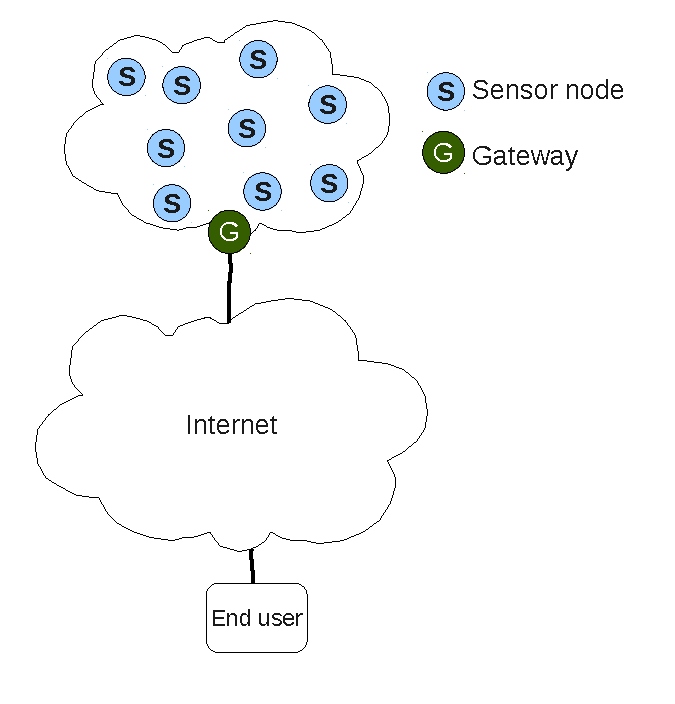
\includegraphics[scale=0.5]
      {Pics/WSNArc.pdf}
   \caption{System architecture for WSN}
    \label{fig:WSNArc}
  \end{center}
\end{figure}

\subsection{The Lower Layers Standard - IEEE 802.15.4}
\label{General:WSN:IEEE}
The physical layer of IEEE 802.15.4 is in charge of data transmission and reception in the physical medium, as well as channel selection and energy management. It operates mainly on three frequency bands: 868-868.6 MHz band for Europe, 902-928 MHz for North America and 2400-2483.5 MHz worldwide. The maximum Service Data Unit (SDU) size that the physical layer is able to receive is 127 octets. 
\newline

Functions of the IEEE 802.15.4 Media Access Control (MAC) layer are: beacon management, channel access, guaranteed time slot management, and data transfer service for upper layers. According to IEEE 802.15.4 definition it can use a 64-bit unique identifier, or a short 16-bit identifier. There are four kinds of frame structures: beacon frame, data frame, acknowledgement frame and MAC command frame. More detailed information about IEEE 802.15.4 can be found in~\cite{IEEE 802.15.4}.
\newline

IEEE 802.15.4 provides wireless communication with short-range, low data-rate communication, low memory requirement, and appropriate power management by defining the physical layer and MAC sub-layer for a low-rate WPAN (LR-WPAN)\@. All these features make IEEE 802.15.4 a promising lower layer protocol for WSNs. 

\subsection{The Network Layer - IPv6}
\label{General:WSN:IPv6}

Being the most accepted network layer protocol, the IP protocol mainly features a universal narrow waist which hides the underlying link technology from the upper layer applications. The traditional IPv4 provides for at most $2^{32}$ addresses. However, judging by the speed of Internet growth, it was predicted that all IP address would soon be exhausted. On July 25, 1994, the IETF proposed IPv6 with $2^{128}$ addresses to be the next generation protocol~\cite{RFC 1752}.
\newline

By implementing IPv6, WSNs can communicate directly with other IP based networks and nodes without intermediate entities. The architecture of a WSN with IPv6 applied is shown in Figure~\ref{fig:Ipv6WSNArc}.
\begin{figure}[htbp]
  \begin{center}
    \leavevmode
      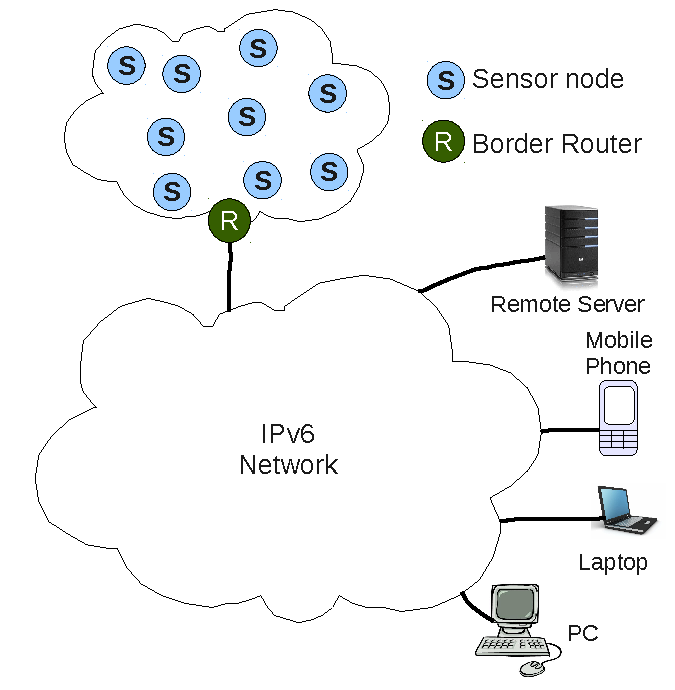
\includegraphics[scale=0.4]
      {Pics/Ipv6WSNArc.pdf}
   \caption{System architecture for WSN with IPv6}
    \label{fig:Ipv6WSNArc}
  \end{center}
\end{figure}
\index{figure 2.2}

Compared with  Figure~\ref{fig:WSNArc}, an IPv6 implemented WSN uses a Border Router (BR) instead of a gateway  to connect the network to the Internet. This kind of network layer router is much more efficient and easier to design than a protocol translating gateway as it eliminates the need for superfluous translations between potentially large number of protocols, which impairs the entire system's usability and usefulness. Furthermore, the 6LoWPAN network can be connected to any other IP based device, giving it extreme adaptability and flexibility unmatched in traditional gateway systems. 
\newline

More advantages of using IPv6 include (but are not limited to):  
\begin{itemize}
 
\item Technologies which use IP are thoroughly researched and known to be safe and reliable.  This saves much effort which would need to be spent in testing and debugging new networking technologies. 
\newline

\item Another reason why IP technologies might prove more suitable are because much of the intellectual rights held by companies in this field are easily traded and used by many players in the field, as opposed to potential lawsuits and legal hassle which might arise due to large-scale usage of new technologies whose intellectual property rights might not be as transparent as the current IP based ones.
\newline

\end{itemize}

As mentioned in Section~\ref{General:WSN:IEEE}, the maximum SDU size that the IEEE 802.15.4 physical layer is able to receive is 127 octets. In the worst-case scenario, this will leave only 81 octets for the MAC layer frame. Meanwhile, IPv6 takes 1280 octets as its Maximum Transmission Unit (MTU) \cite{RFC 4919}. How to fit this 1280 octets IP datagram into a much smaller MAC frame was one of the big concerns. To solve the  size incompatibility and other problems brought by integration of IPv6 and WSN, IETF proposed a series of standards which will be presented in the next chapter.

%}}}

%{{{ Emacs Local Variables

% Local Variables: 
% mode: latex
% TeX-master: "studentprojectthesis"
% TeX-command-list: (("TeX" "tex '\\nonstopmode\\input %t'" TeX-run-TeX nil t) ("TeX Interactive" "tex %t" TeX-run-interactive nil t) ("LaTeX" "%l '\\nonstopmode\\input{%t}'" TeX-run-LaTeX nil t) ("LaTeX Interactive" "%l %t" TeX-run-interactive nil t) ("LaTeX2e" "latex2e '\\nonstopmode\\input{%t}'" TeX-run-LaTeX nil t) ("SliTeX" "slitex '\\nonstopmode\\input{%t}'" TeX-run-LaTeX nil t) ("View" "%v " TeX-run-background t nil) ("Print" "%p " TeX-run-command t nil) ("Queue" "%q" TeX-run-background nil nil) ("File" "dvips %d -o %f " TeX-run-command t nil) ("BibTeX" "bibtex %s" TeX-run-BibTeX nil nil) ("Index" "makeindex -s indexeng.ist %s" TeX-run-command nil t) ("Check" "lacheck %s" TeX-run-compile nil t) ("Spell" "<ignored>" TeX-run-ispell nil nil) ("Other" "" TeX-run-command t t) ("Makeinfo" "makeinfo %t" TeX-run-compile nil t) ("AmSTeX" "amstex '\\nonstopmode\\input %t'" TeX-run-TeX nil t) ("GloTeX" "glotex %t" TeX-run-command nil nil))
% folded-file: t
% End: 

%}}}

\chapter{IETF Standards}
\label{IETF}
The constraints presented in Section~\ref{General:WSN} and the difficulties combining IPv6 with WSN are significant. To realize it, the various working group of IETF have proposed a series of standards in order to solve the problems.

\section{Adaptation Layer: 6LoWPAN}
\label{Intr:6LoWPAN}
The IETF introduced an IPv6 over Low power Wireless Personal Area Networks (6LoWPAN) model, which allows for IPv6 packets to be transmitted or received by the IEEE 802.15.4 network. The detailed specification can be found in \cite{RFC 4944}.
\newline

Instead of the traditional IP based model, a 6LoWPAN protocol stack adds the 6LoWPAN adaptation layer under the IP network layer. Figure \ref{fig:node stack} shows the protocol stacks of a typical 6LoWPAN node and a 6LoWPAN Border Router (6LBR)\@. The protocol stack for 6LoWPAN Border Router (6LBR) is shown in Figure~\ref{fig:6LBR stack}.

\begin{figure}[htbp]
  \begin{center}
    \leavevmode
    \subfloat[Typical 6LoWPAN Node]{\label{fig:node stack}
      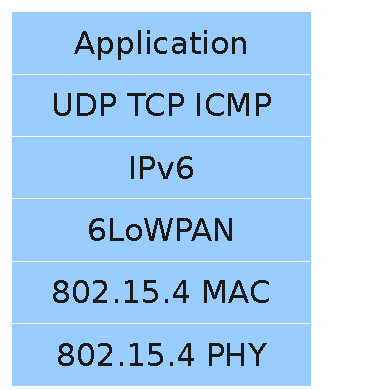
\includegraphics[scale=0.8]{Pics/Protocol.pdf}}
    \subfloat[6LBR]{\label{fig:6LBR stack}
       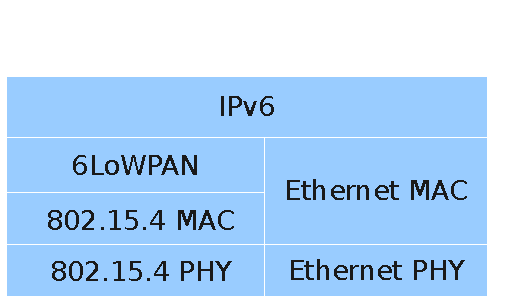
\includegraphics[scale=0.8]{Pics/6LBR.pdf}}
    \caption{Protocol stack of 6LoWPAN nodes}
    \label{fig:protocol stack}
  \end{center}
\end{figure}
\index{figure 3.1}

A 6LBR is a network layer router; when packets are routed though the 6LBR to an external IPv6 based network, the adaptation layer in the LBR translates the LoWPAN format header into a full IPv6 format, and
vice versa. In some practical applications, the adaptation layer is implemented along with an IP
layer such as, for example, in BLIP on the WSN nodes.
\newline

In the adaptation layer, IPv6 header compression and data fragmentation will be performed to solve the problem of frame size incompatibility, and along with layer-two forwarding~\texttt{mesh-under}, it would allow IPv6 packets to be transmitted via the 802.15.4 network. The basic 6LoWPAN frame structure is shown in Figure~\ref{fig:Frame}.  

\begin{figure}[htbp]
  \begin{center}
    \leavevmode
    %\framebox{
     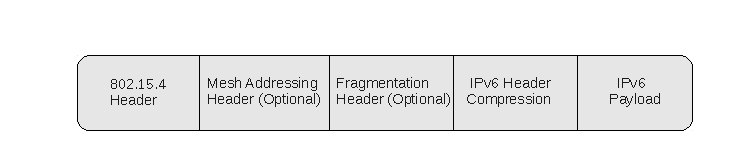
\includegraphics[scale=1]{Pics/Frame.pdf}%}
    \caption{The basic 6LoWPAN frame structure}
    \label{fig:Frame}
  \end{center}
\end{figure}
\index{figure 3.2}

\subsection{Header Compression}
\label{IETF:HC}
The first scheme performed is IPv6 header compression. The idea is to eliminate the
header which contains information of the 6LoWPAN network. That is precisely the reason why it was called stateless header compression. There are two compression formats: header compression one (HC1) and header compression two (HC2)\@. HC1 and HC2 are respectively responsible for the IPv6 header and transport protocol header.  First, the HC1 reduces the 40 octets IPv6 overhead into 2 octets (1 octet for the HC1 encoding and 1 octet for the hop limit)\@. The HC2 is then used to compress any overhead brought by transport layer protocols such as, for example, UDP, TCP, or ICMP.

\subsection{Packet Fragmentation}
\label{IETF:PF}

\begin{figure}[htbp]
  \begin{center}
    \leavevmode
    %\framebox{
    \subfloat[First Fragment]{\label{fig:Fragmentation_1}
      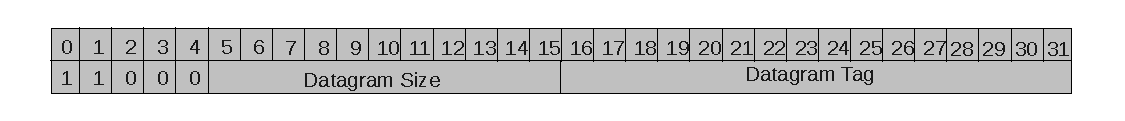
\includegraphics[scale=0.8]{Pics/Fragmentation_1.pdf}}\\
    \subfloat[Subsequent Fragment]{\label{fig:Fragmentation_2}
       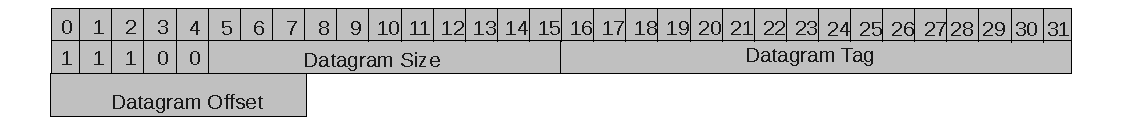
\includegraphics[scale=0.8]{Pics/Fragmentation_2.pdf}}
    \caption{Fragmentation header of 6LoWPAN}
    \label{fig:Fragmentation}
  \end{center}
\end{figure}
\index{figure 3.3}

In front of the compressed IPv6 header there is a fragmentation header (Figure~\ref{fig:Frame})\@. This fragmentation header is only introduced when an IPv6 payload does not fit into a single IEEE 802.15.4 frame;
the payload then needs to be fragmented into several packets. It is used in order to indicate the proper order of the sequences. Figure~\ref{fig:Fragmentation_1} gives the header format for the first
fragment; the header format for subsequent fragments is given in Figure~\ref{fig:Fragmentation_2}.
\newline

When using the routing mechanism~\texttt{mesh-under} (in contrast to~\texttt{route-over}, which forwards packets using IP layer addresses)\@, a mesh addressing header precedes the fragmentation header. Because the source and destination addresses in IPv6 headers are compressed in header compression, this mesh addressing header is needed for packets to be correctly forwarded in a layer-two fashion. The mesh addressing header format with short 16-bit link layer addresses is shown in Figure~\ref{fig:Mesh} (the mesh addressing header with EUI 64-bit addresses has the same format)\@. The first bit and second bit indicates that this header is mesh type. The V bit indicates the originator address (V in this case stands for Very First) being a short 16-bit or an EUI 64-bit address, while F (for Final) bit represents that of the destination address.  This is then followed by a 4-bit section which indicates the numbers of hops remaining and, finally, the link layer addresses for source and destination are added.
\begin{figure}[htbp]
  \begin{center}
    \leavevmode
    %\framebox{
      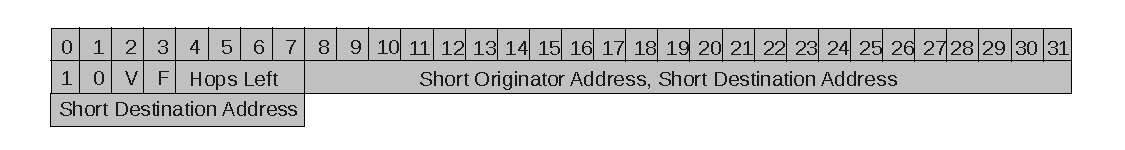
\includegraphics[scale=0.8]{Pics/Mesh.pdf}%}
    \caption{Mesh addressing header of 6LoWPAN}
    \label{fig:Mesh}
  \end{center}
\end{figure}
\index{figure 3.4}

\section{Routing Protocol for Low power and Lossy Networks}
\label{RPL}
IPv6 Routing Protocol for Low power and lossy networks (RPL) as a mesh routing protocol was described by IETF in~\cite{draft-ietf-roll-rpl-19}. RPL is designed to meet the requirements such as: routing requirements for urban (\cite{RFC 5548})\@, industrial (\cite{RFC 5673})\@, home automation (\cite{RFC 5826}) and building automation (\cite{RFC 5867}) usages\@. In RPL the routing objectives, such as minimizing energy, minimize latency, etc., are separately defined in Objective Functions (OFs)\@. It makes RPL flexible to a wider range of Low power and Lossy Networks (LLNs)\@.

\subsection{Topology}
\label{RPL:Topology}

\begin{figure}[htbp]
  \begin{center}
    \leavevmode
      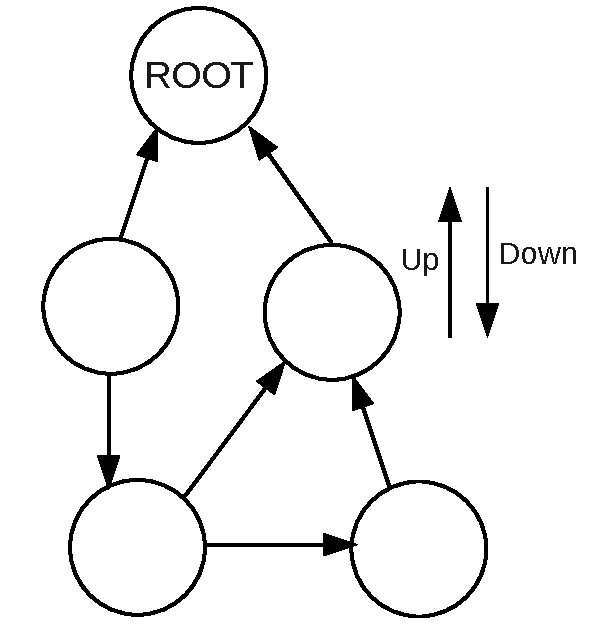
\includegraphics[scale=0.4]{Pics/DODAG.pdf}
    \caption{DODAG}
    \label{fig:DODAG}
  \end{center}
\end{figure}
\index{figure 3.5}
The most basic routing topology RPL forms and maintains is a Destination Oriented Directed Acyclic Graph (DODAG)\@. Figure~\ref{fig:DODAG} shows how a DODAG would look like: it consists of only one root node and has no loop back cycles. There are two directions defined - up which indicates the path towards the root; down which indicates the path away from the root. In a DODAG, a parent of a node is one of the immediate successors of the node on a path towards the DODAG root. 
\newline

Four types of identifier are used in RPL:
\begin{itemize}
\item RPLInstanceID: ID of a set of one or more DODAGs with the same OF called an RPL instance.
\newline

\item DODAGID: unique ID for each DODAG in a RPL instance.
\newline

\item DODAGVersionNumber: ID for each version of a constructed DODAG. Figure \ref{fig:DODAGVersion} shows an example of a DODAG version change.
\newline

\item Rank: a scalar representation of the relative node position with respect to the DODAG root in a DODAG version. A DODAG parent's rank is lower than the node's. Rank helps RPL nodes to detect loops and verify forward progression toward the destination. An simple example is shown in Figure~\ref{fig:Rank}.
\end{itemize}

\begin{figure}[htbp]
  \begin{center}
    \leavevmode
      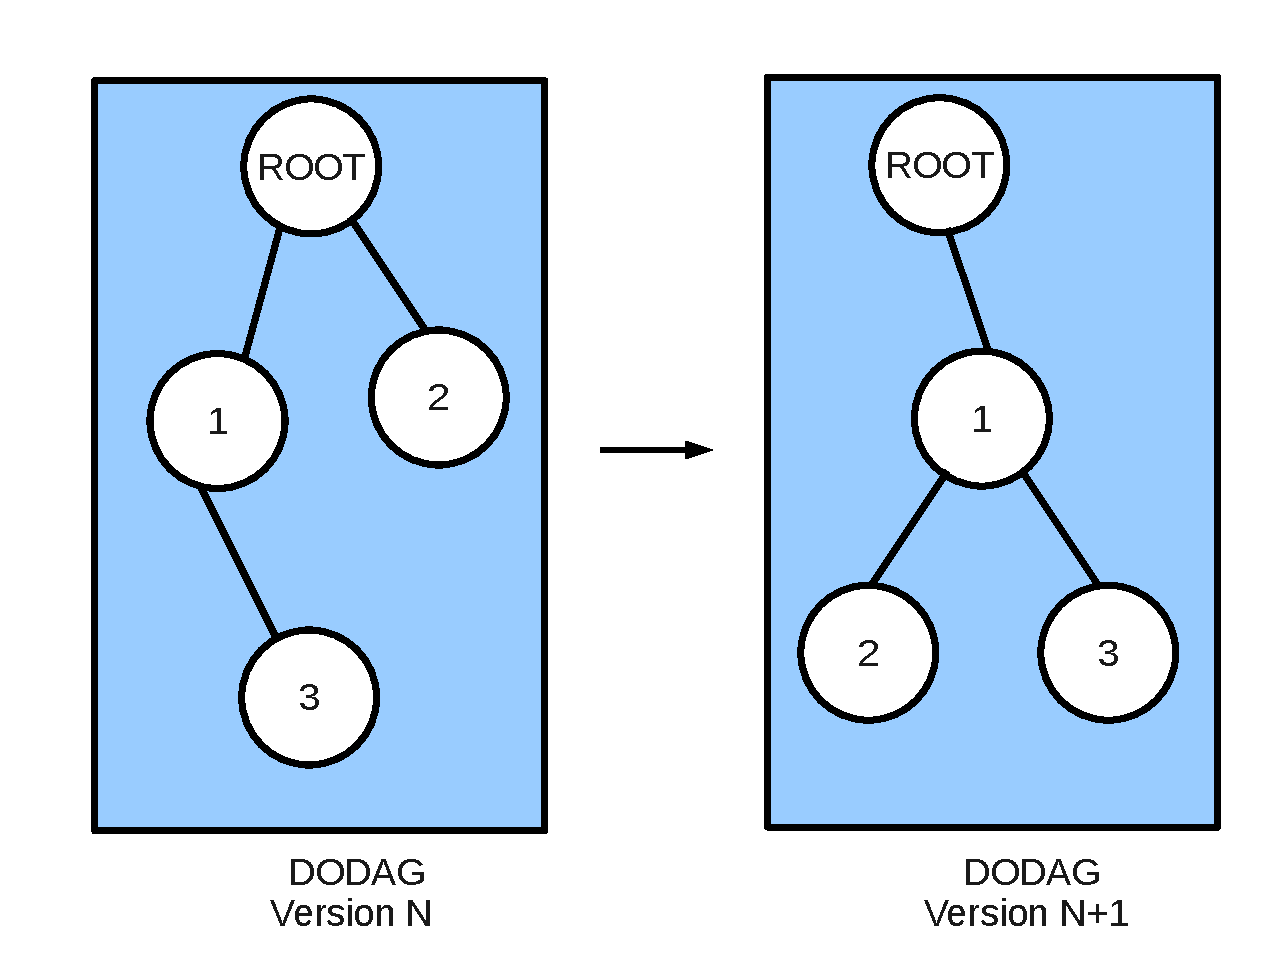
\includegraphics[scale=0.3]{Pics/DODAGVersion.pdf}
    \caption{Node 2 decides to choose node 1 as its parent instead of root which causes a DODAG reconstruction, thus the DODAG version change.}
    \label{fig:DODAGVersion}
  \end{center}
\end{figure}
\index{figure 3.6}

\begin{figure}[htbp]
  \begin{center}
    \leavevmode
      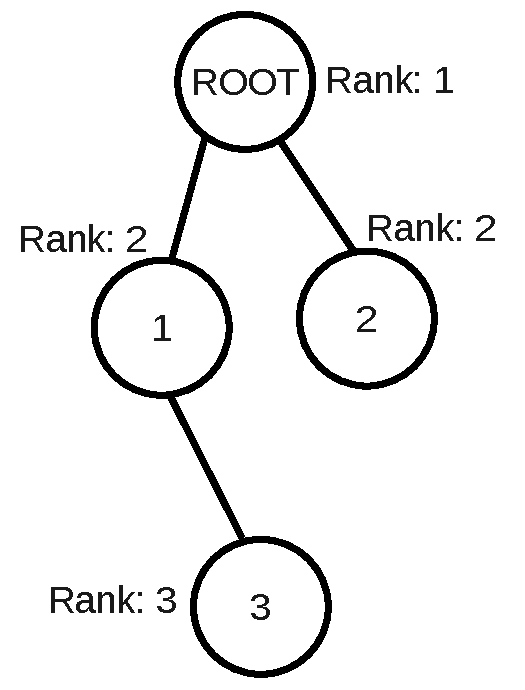
\includegraphics[scale=0.35]{Pics/Rank.pdf}
    \caption{Node 3 has a bigger rank than node 1 and 2, meaning that node 3 is further from the root node than node 1 and 2.}
    \label{fig:Rank}
  \end{center}
\end{figure}
\index{figure 3.7}

The pair of RPLInstanceID and DODAGID defines a unique DODAG, Figure \ref{fig:InstanceID} illustrates the relationship between RPL instance and DODAGs. 
The triple of RPLInstanceID, DODAGID and RPLVersionNumber uniquely identifies a DODAG version.

\begin{figure}[htbp]
  \begin{center}
    \leavevmode
      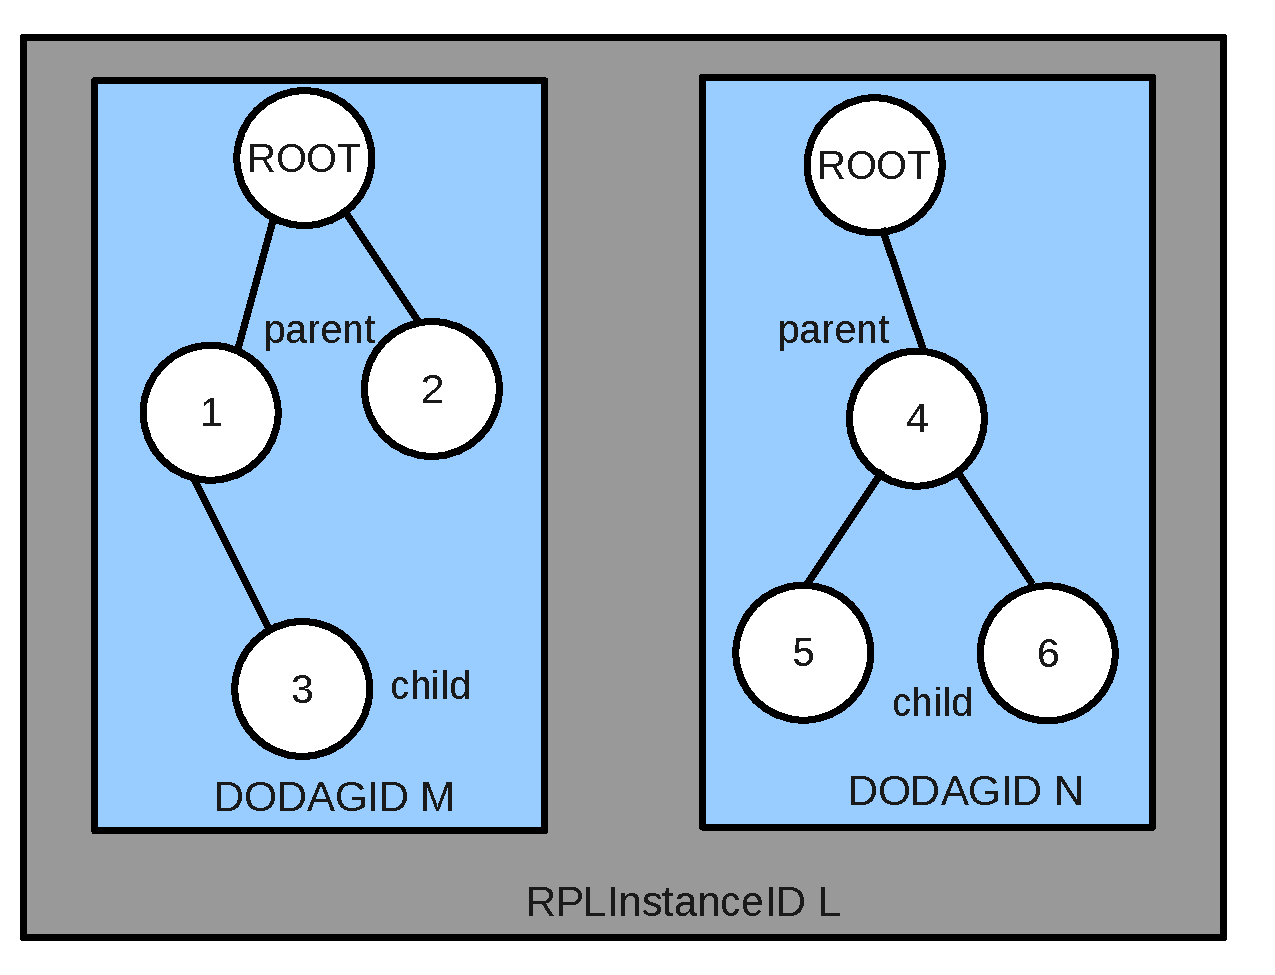
\includegraphics[scale=0.25]{Pics/InstanceID.pdf}
    \caption{A single RPL instance L includes two DODAGs with DODAGID M and N}
    \label{fig:InstanceID}
  \end{center}
\end{figure}
\index{figure 3.8}

\subsection{ICMPv6 Control Messages for RPL}
\label{RPL:ICMP}

As the DODAG has two directions - up and down, there are two kinds of routes defined in RPL: upward routes and downward routes. Upward routes are the routes from a child node to a root node. Similarly, downward routes are the routes which are away from the root to a child node. To maintain these routes, 5 new types of ICMPv6 control messages are used:

\begin{itemize}
\item DODAG Information Solicitation (DIS): DIS is used by a non-root node to request some DODAG information from the neighboring nodes. The neighbors response to a DIS with a DODAG Information Object (DIO) which is the second type of ICMPv6 message used in RPL.
\newline

\item DODAG Information Object (DIO): Information such as node rank, RPL instance ID, DODAG version number are communicated between nodes within DIO messages. It allows the recipient to join a DODAG and choose its parent set and preferable parent according to the OF, metrics and constraints which are carried in the metric container option. The sending of DIO can be triggered by both a Trickle timer or in receiving a DIS.
\newline

\item Destination Advertisement Object (DAO): DAO is typically unicasted by a non-root node to its DAO parent in order to discover and maintain downward routes. DAO sending will be triggered in case of receiving a DIO or receiving a DAO message which is considered new by the recipient.
\newline

\item Destination Advertisement Object Acknowledgement (DAO-ACK): The DAO-ACK message is unicasted by recipient to acknowledge the receiving of the unicast DAO.
\newline

\item Consistency Check (CC): This message protects against replay attacks and synchronize counters. It is related to the secured RPL transmission.
\end{itemize}
%\newline

Figure~\ref{fig:DIS/DIO/DAO} shows basic DIS-DIO and DAO message exchanges. In Figure~\ref{fig:seqence_shot_DIO}, a RPL node sends a DIS to its neighbor and the neighbor will reply with a DAO message. In Figure~\ref{fig:seqence_shot_DAO}, a child sends a DAO message upwards to its parent, and the parent forwards the message to its parent until it reaches the DADAG root.  

\begin{figure}[htbp]
  \begin{center}
    \leavevmode
    %\framebox{
    \subfloat[DIS-DIO]{\label{fig:seqence_shot_DIO}
      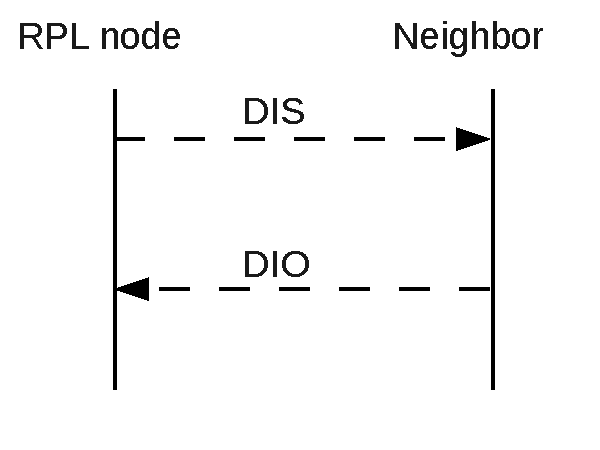
\includegraphics[scale=0.3]{Pics/DIS_DIO.pdf}}\\
    \subfloat[DAO]{\label{fig:seqence_shot_DAO}
       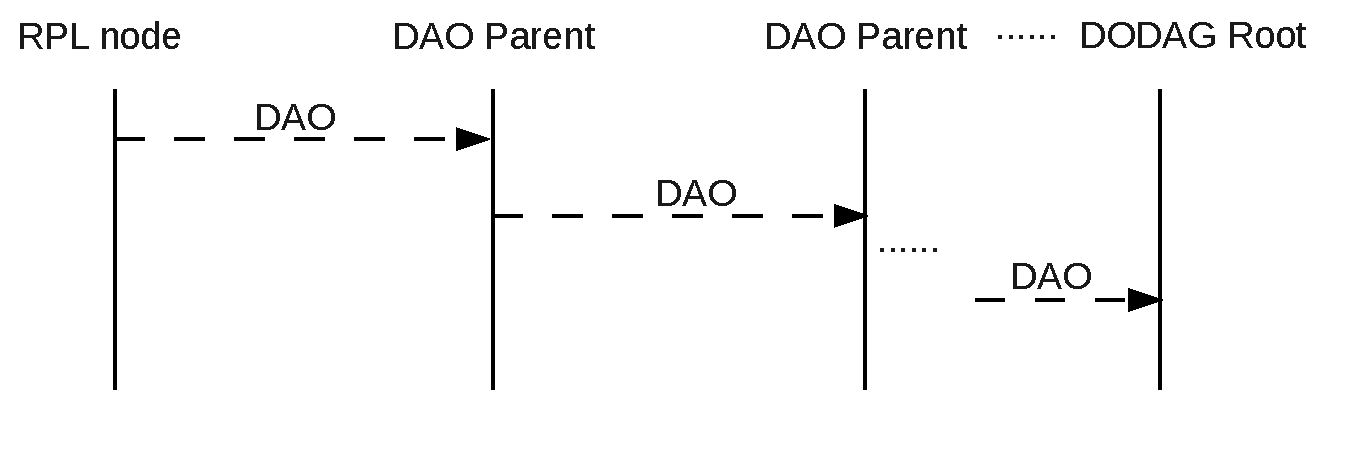
\includegraphics[scale=0.3]{Pics/DAO.pdf}}
    \caption{Basic DIS, DIO and DAO communication}
    \label{fig:DIS/DIO/DAO}
  \end{center}
\end{figure}
\index{figure 3.9}

\subsection{RPL Objective Function}
\label{RPL:OF}
The nodes running RPL might use a number of metrics to describe a link or a node and make it available for route selection. These metrics are advertised in DIO messages using a Metric Container sub-option. An objective function can use these metrics to calculate rank, choose parents and therefore choose routes \cite{MRHOF}. The actual algorithm is implementation-dependent.

\subsubsection{Objective Function Zero}
\label{RPL:OF0}
The Objective Function Zero (OF0) is a very basic type of OF defined in \\ \cite{draft-ietf-roll-of0-19}. OF0 computes rank and selects parent without the guarantee that the resulting path will be optimized according to a specific metric. OF0 is the default OF in RPL.
 
\subsubsection{The Minimum Rank Objective Function with Hysteresis}
\label{RPL:MRHOF}
The Minimum Rank Objective Function with Hysteresis (MRHOF)\, is designed to find the paths with the smallest path cost while preventing excessive churn in the network. It does so by finding the minimum cost path and switching to that path only if it is shorter (in terms of path cost) than the current path by at least a given threshold \cite{MRHOF}. 
\newline

The path cost in MRHOF is defined as the quantitated property of an end-to-end path, and is obtained by summing up the selected metric of the links or nodes along the path. If a DIO doesn't advertise a metric container, MRHOF uses the expected transmission count metric (ETX) as its metric. The ETX metric allows RPL to find the stable minimum-ETX paths from the nodes to a root in the DODAG instance. The rank of a node in MRHOF is directly associated with the path cost of the worst parent in the parent set.

\section{RPL Control Message Timer - the Trickle Timer}
\label{Trickle}
In Section~\ref{RPL:ICMP}, the Trickle timer is mentioned as the control timer for sending DIOs. A Trickle timer uses the Trickle algorithm (\cite{RFC 6206}) to control sending messages which carries information such as routing state, network configuration, etc. The general idea of the Trickle algorithm is: if a node receives a Trickle message and finds out the information, for example, a certain version number, in the message is different from its own and an inconsistency is detected, the Trickle timer will be reset; if the information agrees and no inconsistency detected, then the Trickle algorithm will slow down the transmission of the Trickle message. The definition for consistency is protocol-dependent. With the Trickle algorithm, on one hand, a node can detect the inconsistency efficiently. On the other hand, when there is no inconsistency, Trickle messages are sent less frequently. It does not only save energy in sensor nodes, but also reduce the traffic load in the network which leads to a low channel occupation. 
\newline

The Trickle algorithm defines a Trickle interval with a minimum time interval size $Imin$ and a maximum time interval size $Imax$. Additionally, the algorithm uses a positive redundancy constant $k$. Besides the three parameters above, Trickle maintains three variables:
\begin{itemize}
 \item $I$, the current interval size within the range of $[Imin, Imax]$
 \newline
 
 \item $t$, a timer valued in range of [$\frac{I}{2}, I$]
 \newline
 
 \item $c$, a counter
\end{itemize}

The Trickle algorithm works in the following way \cite{RFC 6206}:
\begin{itemize}
\item For sending:
  \begin{itemize}
  \item First the algorithm begins the time interval $I$, and sets counter $c$ to 0, the timer period $t$ to a random point in the range of $[\frac{I}{2}, I)$.
  
  \item At time $t$, Trickle transmits if and only if the counter $c$ is less than the redundancy constant $k$.
  
  \item When the interval $I$ expires, Trickle doubles $I$ size(up to $Imax$), and picks a new $t$ from range $[\frac{I}{2}, I)$. 
  \end{itemize}  
  
\item For receiving:
 \begin{itemize}
 \item If Trickle hears a message with a consistent information, it increases the counter $c$.
 
 \item If it hears an inconsistency, it resets its Trickle timer to $I=Imin$.
 \end{itemize}
\end{itemize}

The idea of the adaptation layer enables the transmission of IPv6 packet over IEEE 802.15.4, and RPL defines how to route packet within a LLN network. The implementation for a 6LoWPAN network with RPL will be introduced in the following chapter.






 






%}}}

%{{{ Emacs Local Variables

% Local Variables: 
% mode: latex
% TeX-master: "studentprojectthesis"
% TeX-command-list: (("TeX" "tex '\\nonstopmode\\input %t'" TeX-run-TeX nil t) ("TeX Interactive" "tex %t" TeX-run-interactive nil t) ("LaTeX" "%l '\\nonstopmode\\input{%t}'" TeX-run-LaTeX nil t) ("LaTeX Interactive" "%l %t" TeX-run-interactive nil t) ("LaTeX2e" "latex2e '\\nonstopmode\\input{%t}'" TeX-run-LaTeX nil t) ("SliTeX" "slitex '\\nonstopmode\\input{%t}'" TeX-run-LaTeX nil t) ("View" "%v " TeX-run-background t nil) ("Print" "%p " TeX-run-command t nil) ("Queue" "%q" TeX-run-background nil nil) ("File" "dvips %d -o %f " TeX-run-command t nil) ("BibTeX" "bibtex %s" TeX-run-BibTeX nil nil) ("Index" "makeindex -s indexeng.ist %s" TeX-run-command nil t) ("Check" "lacheck %s" TeX-run-compile nil t) ("Spell" "<ignored>" TeX-run-ispell nil nil) ("Other" "" TeX-run-command t t) ("Makeinfo" "makeinfo %t" TeX-run-compile nil t) ("AmSTeX" "amstex '\\nonstopmode\\input %t'" TeX-run-TeX nil t) ("GloTeX" "glotex %t" TeX-run-command nil nil))
% folded-file: t
% End: 

%}}}

\chapter{The 6LoWPAN Implementation - BLIP/TinyOS}
\label{Blip/TinyOS}
There are several implementations for 6LoWPAN, such as uIPv6, BLIP, Sensinode's NanoStack, Jennic's 6LoWPAN and Nivis ISA100. The first two are open-source protocol stacks
for the embedded operating systems, Contiki and TinyOS. The latter are commercial protocol
stacks~\cite{ShelbyBormann2009}. Among all those implementations, BLIP for TinyOS is well known and respected implementation due to its many useful applications. Using BLIP/TinyOS, one is able to form multi-hop IP networks consisting of different nodes \cite{BLIP}. Simulation of BLIP/TinyOS is the main focus of the research of this paper.

\section{TinyOS}
\label{TinyOS}
TinyOS is a light-weight open source operating system designed for low-power wireless devices, such as those used in sensor networks, ubiquitous computing, personal area networks, smart buildings, and smart meters \cite{TinyOS}. It allows for various applications to be installed on sensor nodes via USB connections. The language that is used in TinyOS is NesC, which is a dialect of the C language. NesC is a component-based as well as event-driven programming language; the components are wired together using interfaces. NesC was designed to make the operating system optimized for the memory constraints of sensors.
\newline

The latest official release is TinyOS 2.1.1. It supports multiple platforms, such as Mica-family, Telos-family, epic, mulle, and shimmer2 platforms. 

\subsection{Radio Stack}
\label{Sim:radio stack}
\begin{figure}[htbp]
  \begin{center}
    \leavevmode
      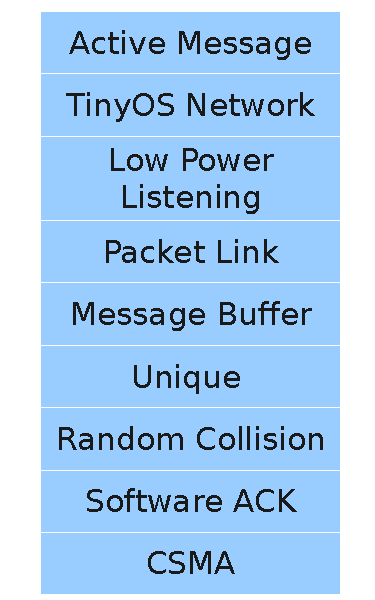
\includegraphics[scale=0.45]{Pics/Rfxlinklayer.pdf}
   \caption{Radio stack for rfxlink}
    \label{fig:rfxlinklayer}
  \end{center}
\end{figure}
\index{figure 4.1}
Different platforms might use different radio chips. For example: Micaz platforms use CC2420 and TelosB, and IRIS uses RF230. Most of the low-level transmission and receiving packets are taken care of by the radio chip hardware, specifying the proper behavior of that hardware requires a well defined radio stack implementation \cite{TEP 126}. 
An new radio stack called rfxlink is added in TinyOS 2.1.1. The rfxlink stack unifies CC2420 and RF230 software radio stacks, and leaves only chip driver part different. It is the future standard radio stack. In addition, TOSSIM support has been added to the rfxlink stack.
The rfxlink radio stack includes several layers which are shown in Figure \ref{fig:rfxlinklayer}. 
\section{The implementation - BLIP}
\label{Blip}
BLIP, short for the Berkeley Low-power IP stack, is an implementation of 6LoWPAN adaptation layer and IP layer. It was included as a core part of TinyOS. 

The main parts of the BLIP implementation consist of:
\begin{itemize}
\item Transport layer: BLIP implements User Datagram Protocol (UDP), Transmission Control Protocol (TCP) and Internet Control Message Protocol (ICMP) in this layer.
\newline

\item Network layer: in this layer, BLIP defines the routing protocol for Low power and Lossy Networks (LLNs), such as HYDRO or RPL.
\newline
 
\item 6LoWPAN adaptation layer: as mentioned in Section \ref{Intr:6LoWPAN}, this layer compress certain higher-level headers and break large packets into multiple link-layer fragments.
\end{itemize}
%\newline

BLIP has been changed considerably since BLIP 1.0. In May 2010, BLIP version 2.0 has been added to the TinyOS repository. 
\subsection{Difference between BLIP 1.0 and BLIP 2.0}
\label{Blip:1.0-2.0}

\begin{figure}[htbp]
  \begin{center}
    \leavevmode
    %\framebox{
    \subfloat[BLIP 1.0]{\label{fig:blip1.0}
      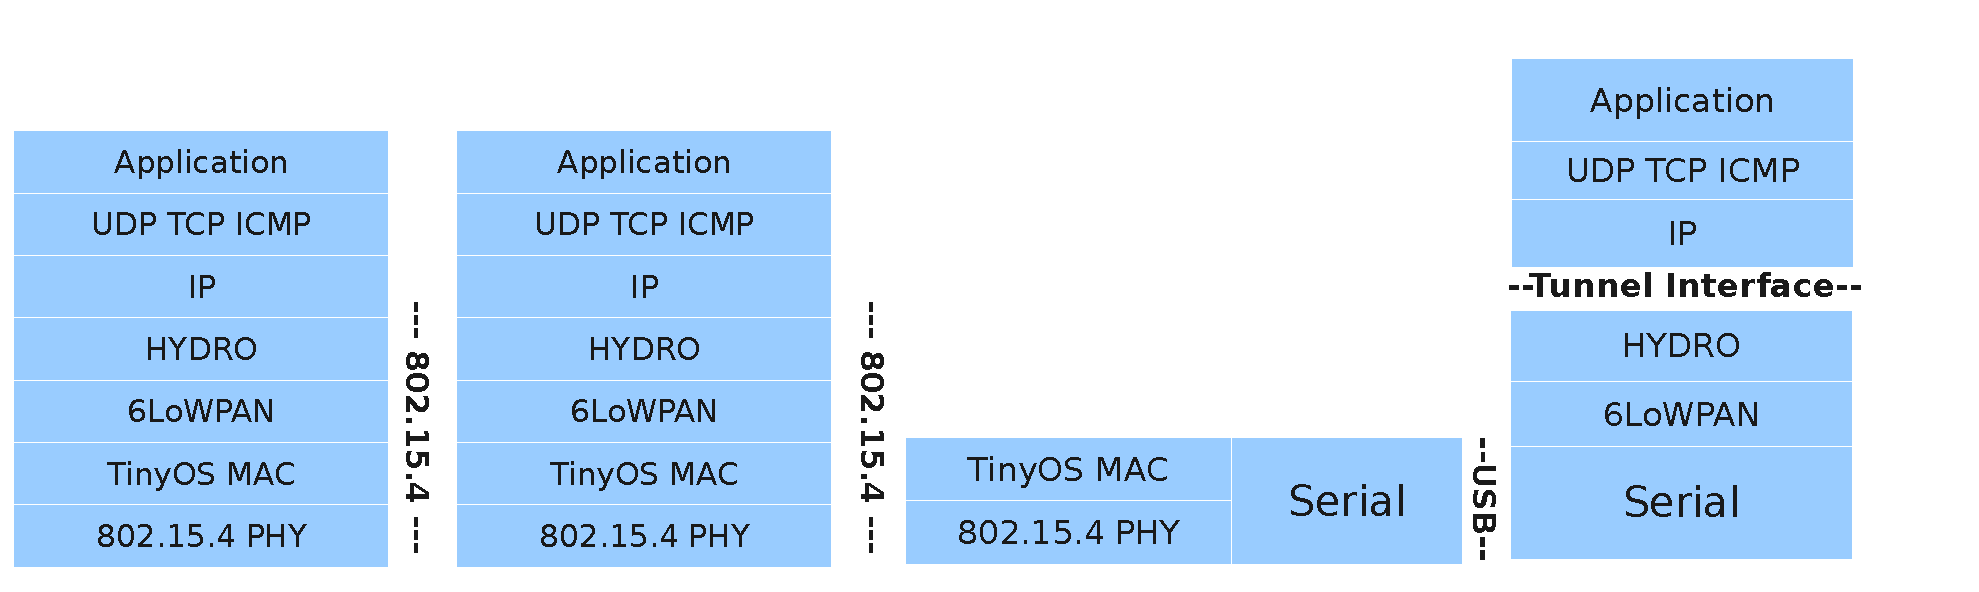
\includegraphics[scale=0.35]{Pics/blip1.pdf}}\\
    \subfloat[BLIP 2.0]{\label{fig:blip2.0}
       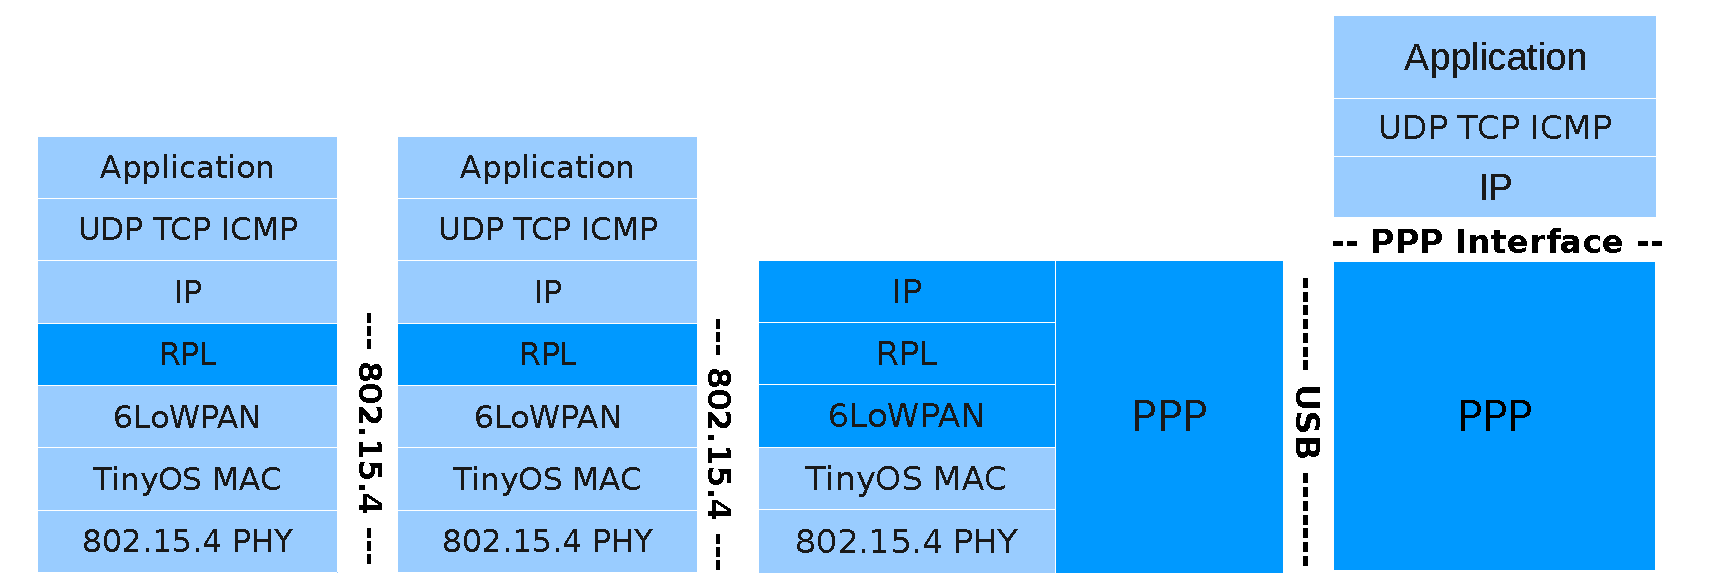
\includegraphics[scale=0.35]{Pics/blip2.pdf}}
    \caption{Protocol stacks for BLIP}
    \label{fig:blip}
  \end{center}
\end{figure}

An overview of the protocol stack for both BLIP implementations can be found in Figure~\ref{fig:blip}. BLIP 2.0 introduces RPL instead of HYDRO as the routing protocol. Compared to HYDRO, RPL employs a more sophisticated way to discover topological changes and react accordingly. Moreover, RPL gives more standard compliance than HYDRO.
\newline

The second main change is in the border router. Version 2.0 employs an IP layer router with a Point-to-Point Protocol (PPP) interface. The PPP interface provides a PPP connection to a normal IP device, which can then perform some higher level functionalities such as data collection.
\newline

Since BLIP 1.0 was updated to BLIP 2.0, the simulation of BLIP had to be re-enabled. The next chapter will give the details about the simulation, including the simulator, enabling the simulation and the scenario setups.


\chapter{Simulation}
\label{Sim}
Network simulation is a practical way of developing and researching networks and their
behaviors. Especially in WSNs, the main focus is not on one particular sensor node, but on
the behavior of the entire network (which can consist of thousands of sensor nodes). It would
be impractical to do initial research based on real world testing and deployment, as that would cost exorbitant amounts of money, and create logistical nightmares in the WSN setup. For this reason a valid
simulation tool is a necessity for further studies. This chapter focuses on the simulation; it 
includes discussion about the simulator, simulation execution, scenario setups and simulation procedure.

\section{TinyOS Simulator - TOSSIM}
\label{Sim:TOSSIM}

The simulator used in this project is called TOSSIM\@. TOSSIM is a discrete, event-driven WSN simulator included in TinyOS. Compiling unchanged TinyOS applications
directly into its framework, TOSSIM can simulate thousands of motes running complete
applications~\cite{LLWC}. It fulfils the requirements of being a TinyOS simulator; such requirements include: scalability, completeness and fidelity. TOSSIM is a shared library, therefore a script written with C++ or Python must be created to run the simulation.  Python is chosen in this thesis as it can dynamically interact with the simulation.

Configuring networks for TOSSIM simulation usually includes setting
up a network topology and an interference model. For the topology, a file with the format~\texttt{Source Destination Gain} needs to be created. TOSSIM uses the Closest Pattern Matching (CPM) algorithm to calculate channel noise. It is a wireless noise simulation model
based on statistical extraction from empirical noise data. It works by taking a noise trace as input to generate the interference model. This method is accepted to be much more accurate and preferable than the traditional, Independent Packet Loss (IPL) models~\cite{TOSSIM}.

\section{Enabling the Simulation}
\label{Sim:Enabling}

The simulation had already been enabled for a multi-hop network using the BLIP 1.0 implementation before. The radio stack for this simulation was the CC2420. But due to the significant changes that were done to both the CC2420 radio stack and BLIP, considerable work was required to re-enable the simulation of BLIP 2.0. 

As mentioned in Section~\ref{Sim:radio stack}, the rfxlink radio stack unifies CC2420 and RF230. Furthermore, the TOSSIM simulation support for rfxlink has been developed by Morten Tranberg Hansen~\cite{rfxsim}. But neither BLIP 1.0 nor BLIP 2.0 have been implemented on top of rfxlink. In oder to execute the simulation, the simulated rfxlink had to be moved underneath BLIP 2.0. 

The re-enabling of the simulation required the following steps: 
\begin{itemize}
\item Merging of the branch of Morten Tranberg Hansen's rfxsim repository~\cite{rfxsim}. 

\item Adding the simulated ``chip driver'' layer - TossimDriverLayerC to the already supported CC2420 and RF230 radio chips of rfxlink. 

\item Introducing 802.15.4 packets into TOSSIM. TinyOS basic packets abstraction is Active Message (AM), but 6LoWPAN uses 802.15.4 packets. Introduction of 802.15.4 packets into TOSSIM is essential for the simulation to run.

\item Configuring the simulation to support BLIP 2.0. Using short IEEE 802.15.4 addresses for \texttt{Ieee154Send} interface in the component \texttt{IPDispatch}. 

\item The compiler GPP is used to compile BLIP 2.0, while the 6LoWPAN library is written in C. The \texttt{extern ``C''} had to be added to notify the C++ compiler of the C style functions.

\item A Makefile had to be written to include 6LoWPAN object files into the simulation library.
\end{itemize}

\section{Simulation Setups}
\label{Sim:Setup}
\subsection{Methodology}
\label{Sim:Method}
The application~\texttt{UDPEcho} is used in the simulation to evaluate the performance of the RPL protocol. It is configured to behave similarly to the application~\texttt{Ping}. A node sends out a data packet to another node, which replies back to the original sender. However, this is done on the application layer. The application is installed on the simulated root node and the child nodes. In the simulation, the root node will send 100 \texttt{UDPEcho} packets one after another to a child node, then continue to send another 100 \texttt{UDPEcho} packets to the next child node, until all child nodes are  ``pinged''.     

The simulation is done for various scenarios with different number of nodes, as well as with objective functions OF0 and MRHOF. The results of the simulation is visualized with the python plotting library~\texttt{Matplotlib}.

\subsection{Simulation Scenarios}
\label{Sim:Scenarios}

Two kinds of scenarios are created for the simulation - a line scenario and a grid scenario. In the line scenario the neighboring nodes are equally distanced; in the grid scenario, the number of nodes should be a square number, and the grids are square grids. Figure~\ref{fig:scenario_line} shows a 4-node line scenario with 10-meter inter-node distance. A 9-node grid scenario with 100-meter inter-node distance is shown in Figure~\ref{fig:scenario_grid}. Node 1 is configured to be the root node in the simulation.

\begin{figure}[htpb]
 % \begin{center}
 	\centering
    \leavevmode
    %\framebox{
      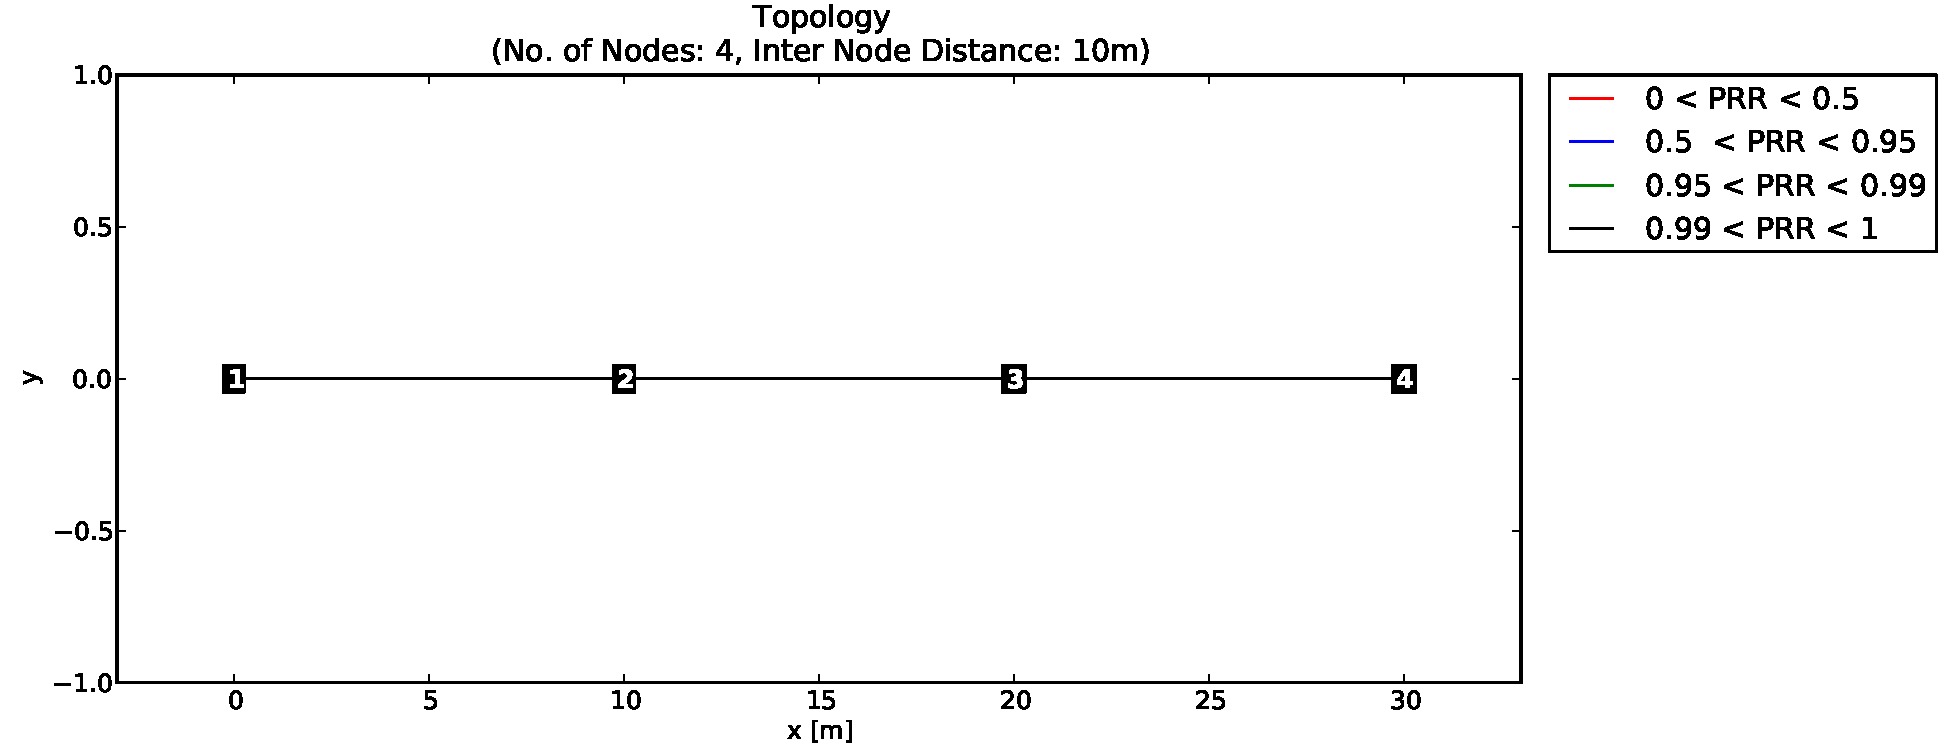
\includegraphics[scale=0.35]{Pics/results/topo4_dist10_line.pdf}
    \caption{Line scenario}
    \label{fig:scenario_line}
\end{figure}

\begin{figure}[htpb]	
%  \begin{center}
  	\centering
    \leavevmode
    %\framebox{
      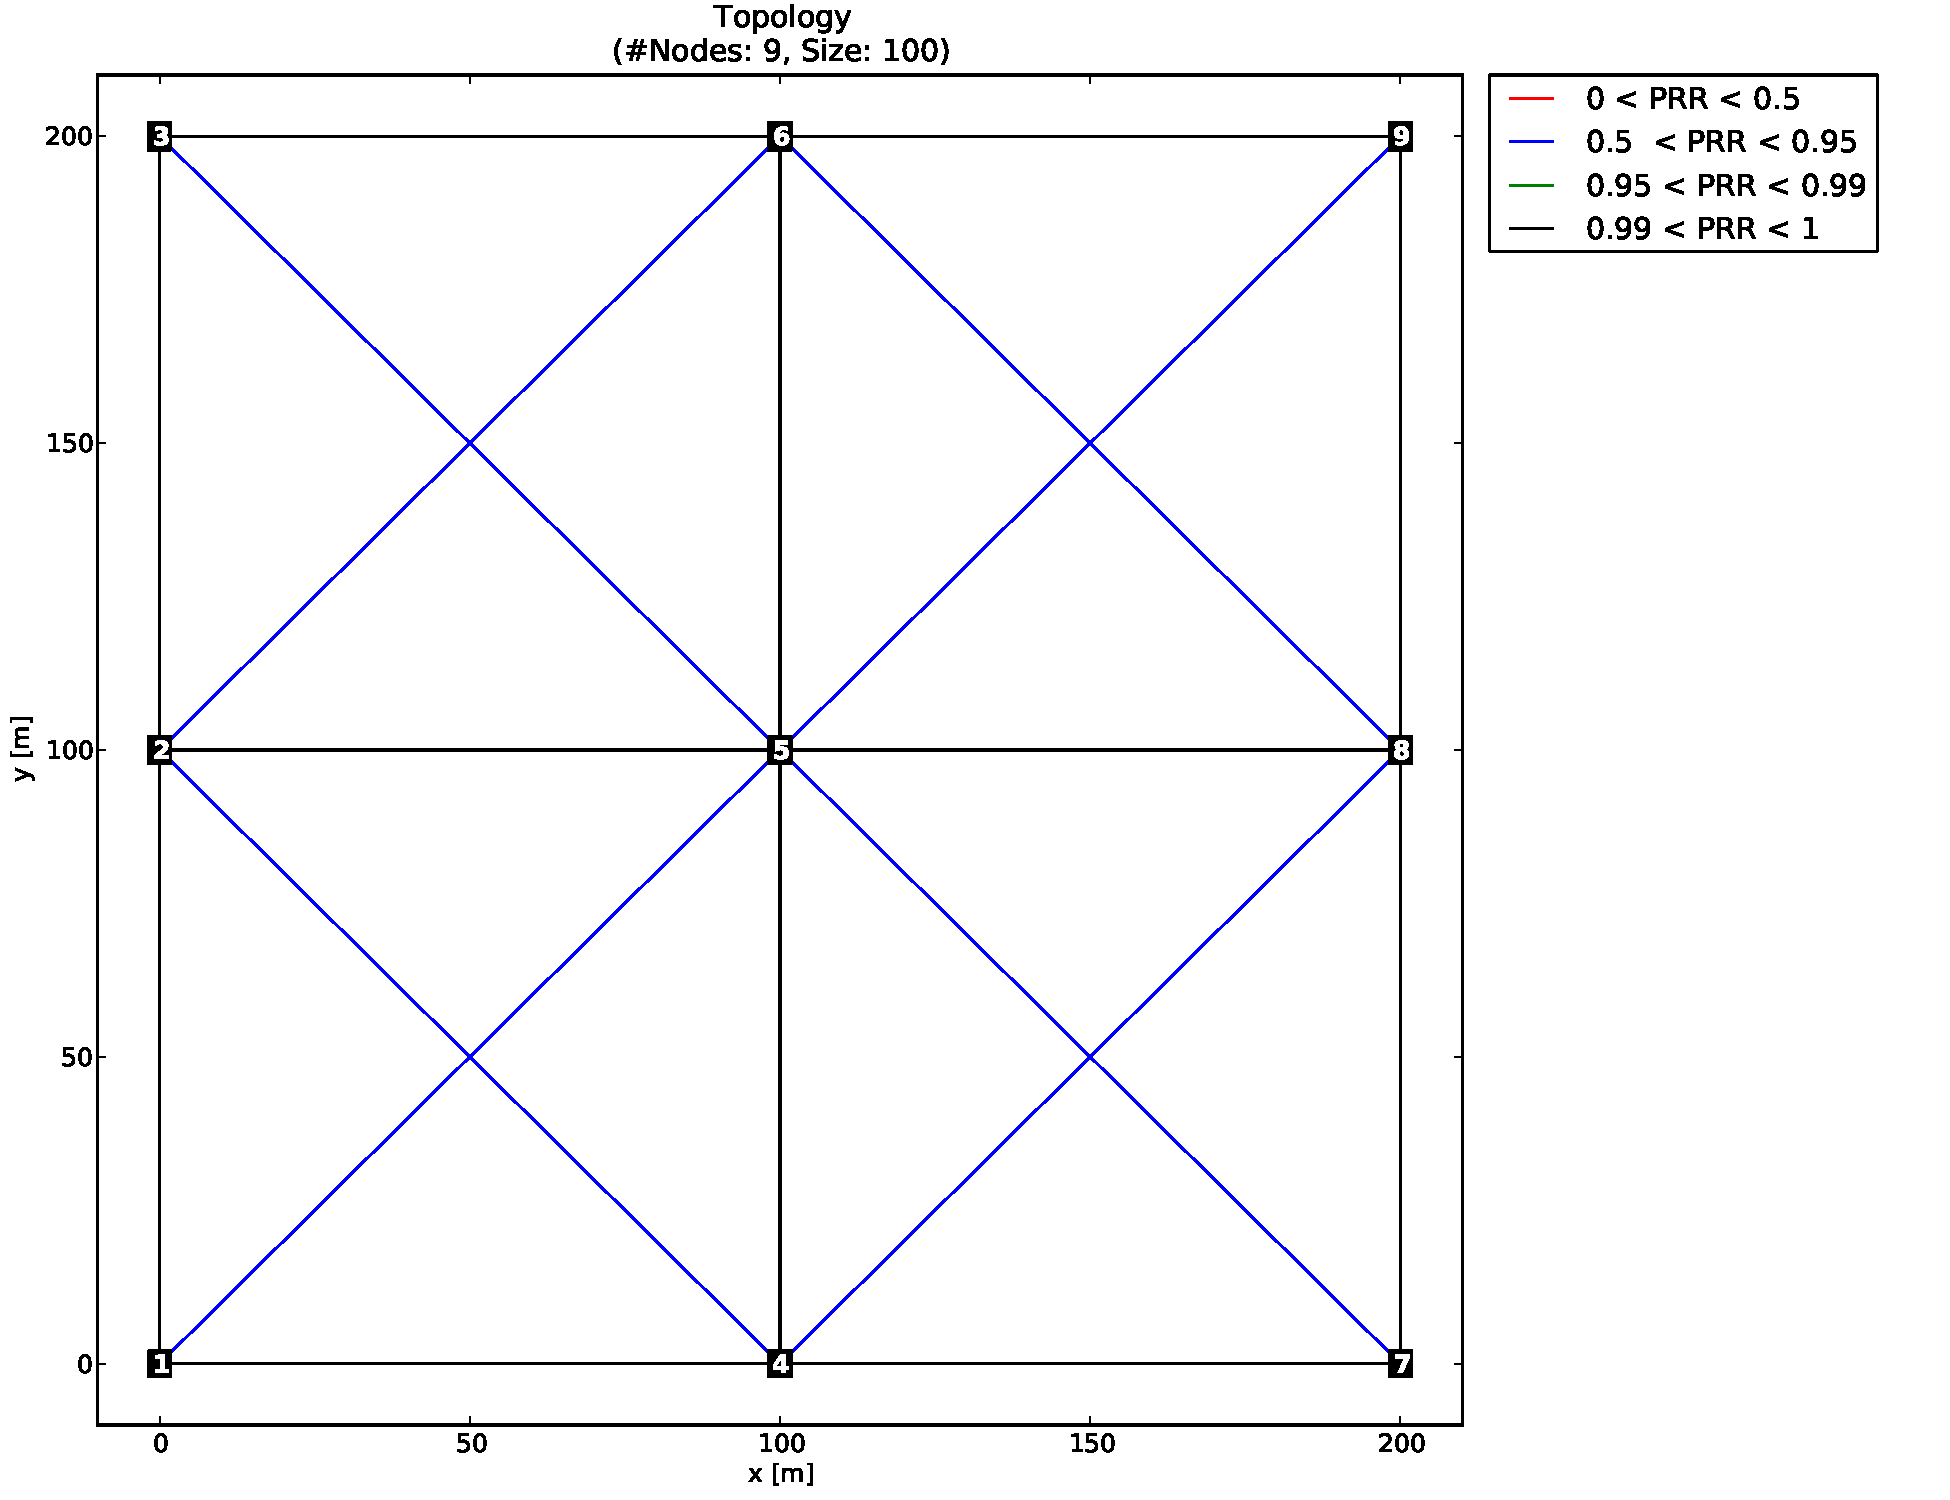
\includegraphics[scale=0.35]{Pics/results/topo9_dist100_grid.pdf}
    \caption{Grid scenario}
    \label{fig:scenario_grid}
%  \end{center}
\end{figure}

The Packet Reception Ratio (PRR) is estimated from Signal-to-Noise Ratio (SNR). The estimation is based on the measurement in~\cite{RL08}:
\[
PRR = (1-0.5*erfc(\frac{\beta_1*(SNR-\beta_2)}{\sqrt{2}}))^{46}
\quad{\beta_1} = 0.9794, {\beta_2} = 2.3851
\] 
with 
\[
SNR = Signal\:(dBm)- Noise\:(dBm) = -(50 + 20 {\log}(Distance)) - (-98)\:(dBm)
\] 
The relationship between distance and PRR is shown in Figure~\ref{fig:prr}. When the distance between two nodes is smaller than 120~m, they can hear each other with a PRR value larger than 0.99. Once the distance is larger than 120~m, the PRR begins to decline until it reaches a value of zero at a distance of 165~m.  This means that at a distance of over 165~m two nodes are at least two hops apart.

\begin{figure}[htbp]
  \begin{center}
    \leavevmode
      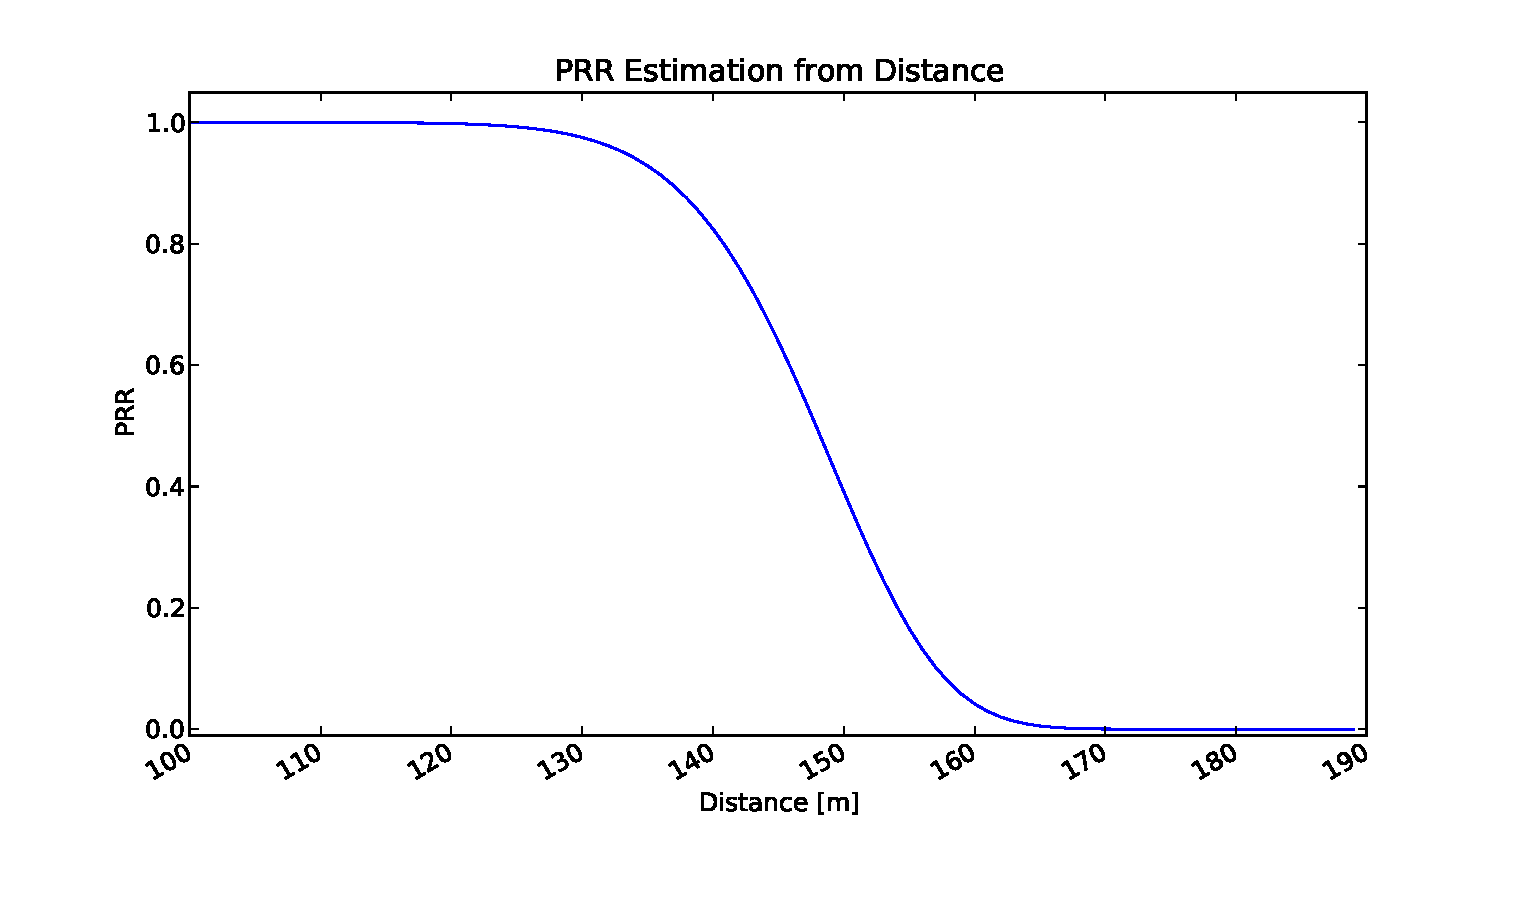
\includegraphics[scale=0.45]{Pics/prr.pdf}
   \caption{Relationship between distance and PRR}
    \label{fig:prr}
  \end{center}
\end{figure}

\subsection{Trickle Parameters and Variables}
\label{trickle parameters}
The Trickle timer parameters and initial variables of RPL in the simulation are set as below:
\begin{itemize}
\item Minimum time interval size $Imin = 256\:ms$;

\item Maximum time interval size $Imax = 262144\:ms = 256\:s$;

\item Redundancy constant $k = 255$;

\item Initial current interval size $I = 256\:ms$;

\item Initial timer value t randomly chosen in range of $[128, 256)\:ms$;

\item Initial counter $c=0$.
\end{itemize}

\subsection{Simulation Metrics}
\label{Sim:metrics}
The metrics that are used to evaluate the RPL performance are:
\begin{itemize}
\item Cumulative distribution function (CDF) of time to default route discovery: when a node receives the first DIO message from a lower rank node, it sets the default route entry. The sending of the DIO is controlled by a Trickle timer. The CDF of the default route discovery time will demonstrate the characteristics of the Trickle algorithm.

\item Mean control message overhead over 100 runs: In order to show the effect of the Trickle timer, the amount of ICMP messages a node sends out during time intervals will be shown.

\item Mean packet loss over 100 runs: Packet loss rate shows the quality of the links between nodes. A good multi-hop routing protocol should be able to forward packet properly to the destination under the certain link condition. The mean packet loss rate of both OF0 and MRHOF will be compared.

\item Mean Round-Trip Time (RTT) over 100 runs: The mean RTT for various scenarios and both OF0 and MRHOF with link ETX (hereinafter referred to as MRHOF) will be evaluated.

\end{itemize}








\chapter{Simulation Result and Evaluation}
\label{ResultandEvaluation}

The simulations were done for both line and grid scenarios, as well as varying number of nodes and internode distances (4, 9, 16 nodes and 10, 50, 100 meters respectively). Furthermore, for each topology both OF0 and MRHOF were simulated. A total of 100 separate simulations were performed for each scenario setup. The simulation results are arranged in four parts according to the different simulation metrics, and each simulation metric is examined for individual scenario setup. 

\section{Packet Loss Rate}
\label{pl}

In the simulation a packet is considered to be lost when the echo packet is not received by the sender(in this case the root). 100 \texttt{UDPEcho} packets are sent from the root to each node in the network.

\subsection{Line Scenario}
\label{pl:line}
Figure \ref{fig:pl_4_line_10} to Figure \ref{fig:pl_4_line_100} show the Mean packet loss rates for the 4-node line scenario with internode distances of 10, 50 or 100 meters. The figures on the left show the results with OF0, and the right ones are the results with MRHOF. In Figure \ref{fig:pl_9_line_10} to Figure \ref{fig:pl_16_line_100}, the mean packet loss rates are presented in the same way for the 6- and 9-node line scenarios.

%%%%%%%%%%%%%%%%%%%%%%%%%%%%%%%%%%%%%%% line 4 %%%%%%%%%%%%%%%%%%%%%%%%%%%%%%%%%%%%%%%%

\begin{figure}[p]
  \centering
    \leavevmode
    \subfloat[OF0]{\label{fig:4/OF0/line/dist10_montecarlo_contour_packetloss}
      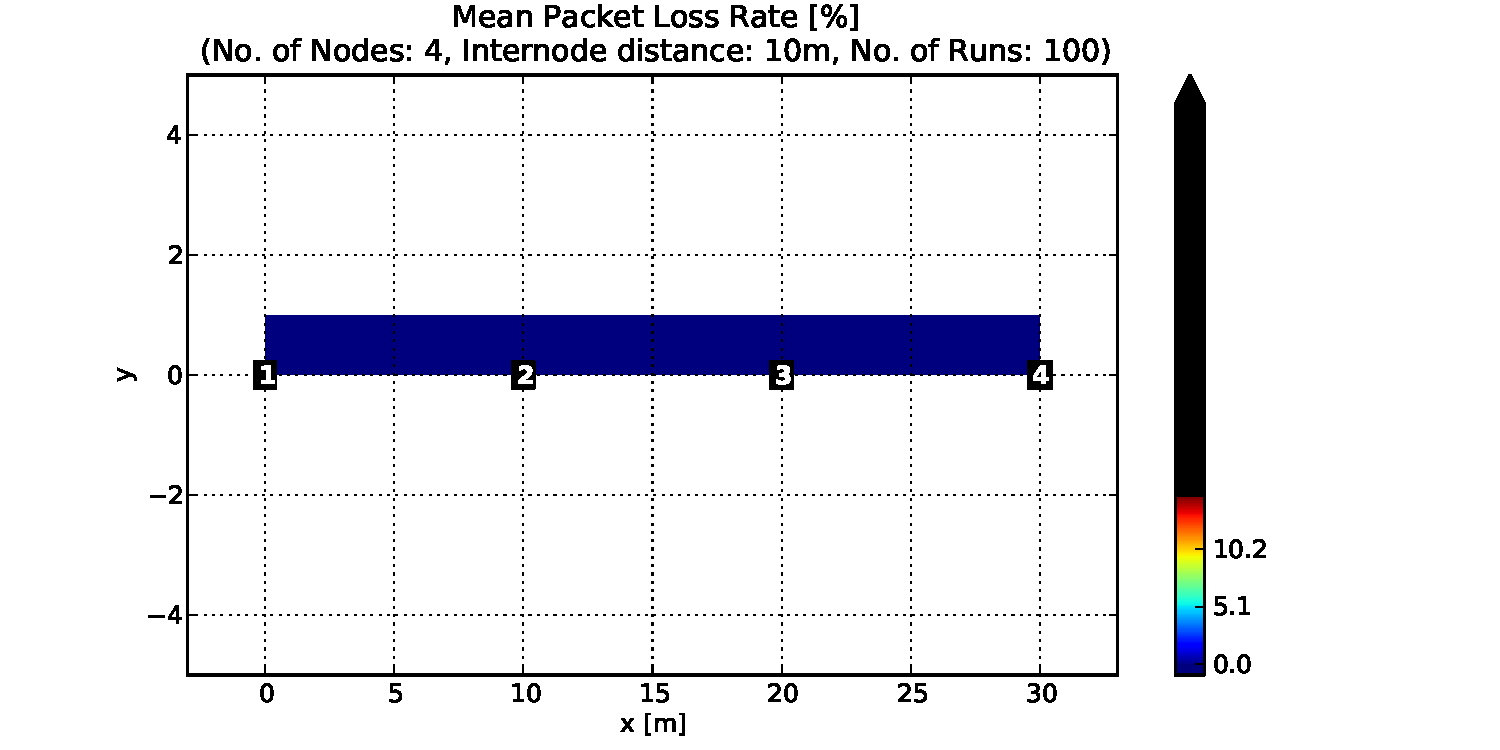
\includegraphics[trim=1.7cm 0cm 3cm 0cm, clip=true, scale=0.38]{Pics/results/4/OF0/line/dist10_montecarlo_contour_packetloss.pdf}}
    \subfloat[MRHOF]{\label{fig:4/MRHOF/line/dist10_montecarlo_contour_packetloss}
      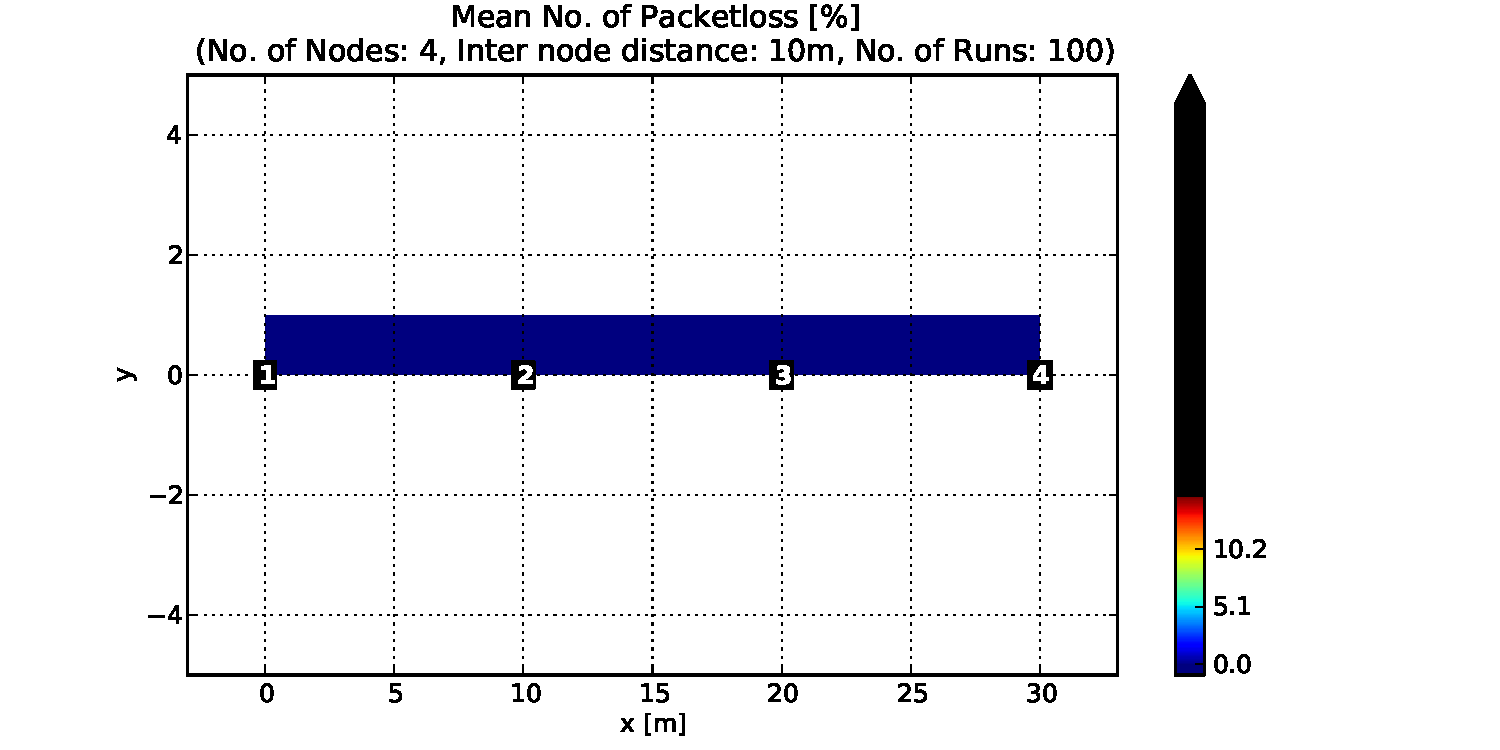
\includegraphics[trim=1.7cm 0cm 3cm 0cm, clip=true, scale=0.38]{Pics/results/4/MRHOF/line/dist10_montecarlo_contour_packetloss.pdf}}
   \caption{Mean packet loss rate: 4-node line scenario with 10 m internode distance}
   \label{fig:pl_4_line_10}
\end{figure}

\begin{figure}[p]
  \centering
    \leavevmode
    \subfloat[OF0]{\label{fig:4/OF0/line/dist50_montecarlo_contour_packetloss}
    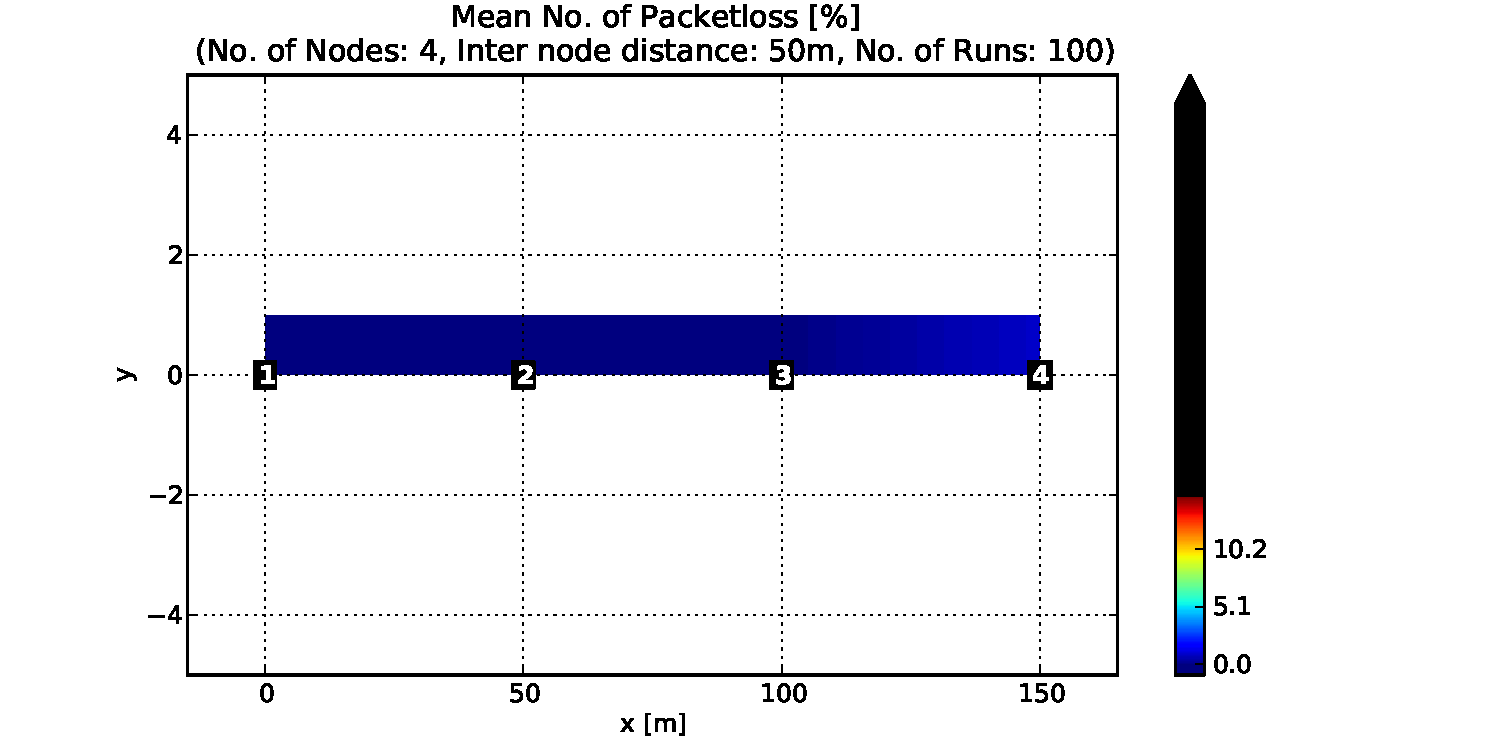
\includegraphics[trim=1.7cm 0cm 3cm 0cm, clip=true, scale=0.38]   {Pics/results/4/OF0/line/dist50_montecarlo_contour_packetloss.pdf}}
    \subfloat[MRHOF]{\label{fig:4/MRHOF/line/dist50_montecarlo_contour_packetloss}
      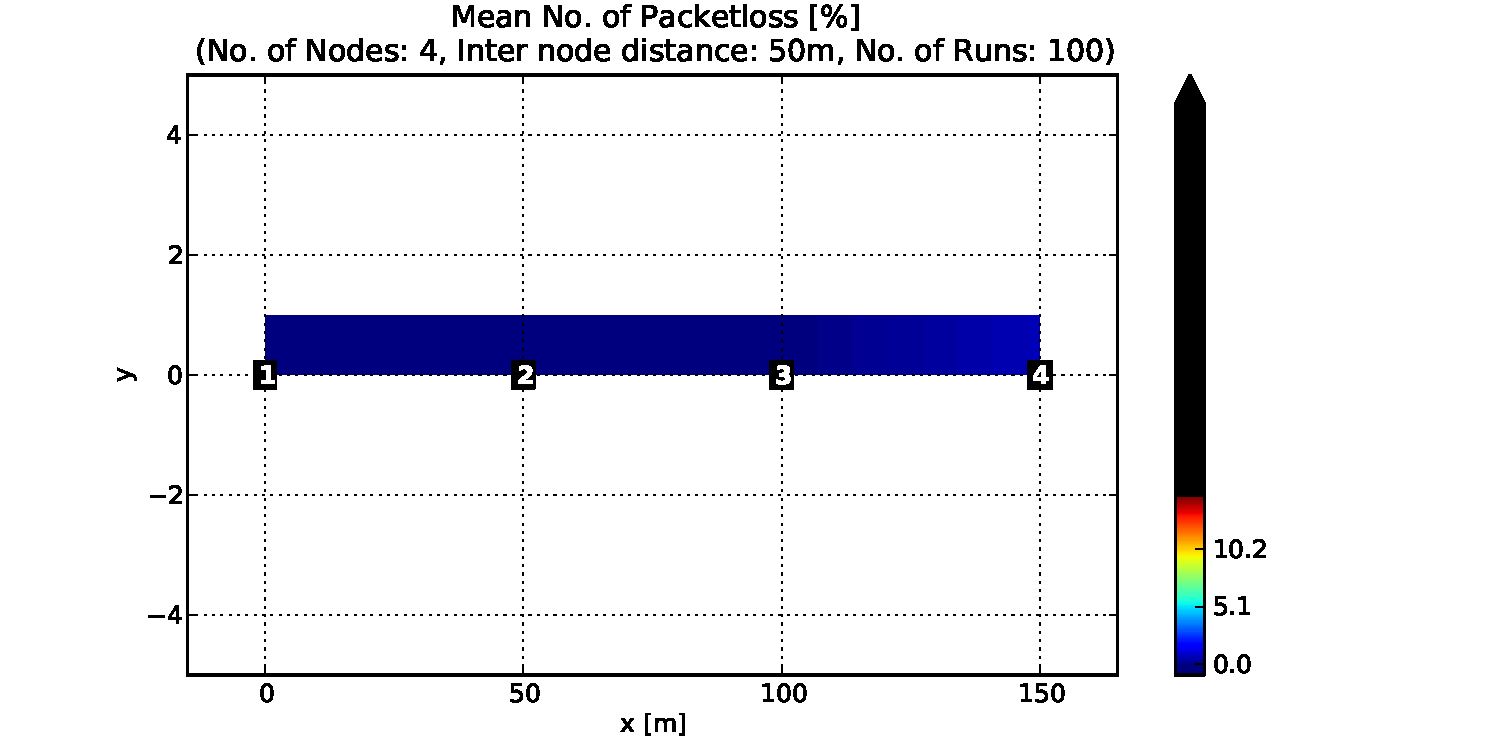
\includegraphics[trim=1.7cm 0cm 3cm 0cm, clip=true, scale=0.38]{Pics/results/4/MRHOF/line/dist50_montecarlo_contour_packetloss.pdf}}
   \caption{Mean packet loss rate: 4-node line scenario with 50 m internode distance}
   \label{fig:pl_4_line_50}
\end{figure}

\begin{figure}[p]
  \centering
    \leavevmode
    \subfloat[OF0]{\label{fig:4/OF0/line/dist100_montecarlo_contour_packetloss}
     \includegraphics[trim=1.7cm 0cm 3cm 0cm, clip=true, scale=0.38]{Pics/results/4/OF0/line/dist100_montecarlo_contour_packetloss.pdf}}
    \subfloat[MRHOF]{\label{fig:4/MRHOF/line/dist100_montecarlo_contour_packetloss}
     \includegraphics[trim=1.7cm 0cm 3cm 0cm, clip=true, scale=0.38]{Pics/results/4/MRHOF/line/dist100_montecarlo_contour_packetloss.pdf}}
  \caption{Mean packet loss rate: 4-node line scenario with 100 m internode distance}
  \label{fig:pl_4_line_100}
\end{figure}
%%%%%%%%%%%%%%%%%%%%%%%%%%%%%%%%%%%%%%% line 9 %%%%%%%%%%%%%%%%%%%%%%%%%%%%%%%%%%%%%%%%
\begin{figure}[p]
  \centering
    \leavevmode
    \subfloat[OF0]{\label{fig:9/OF0/line/dist10_montecarlo_contour_packetloss}
      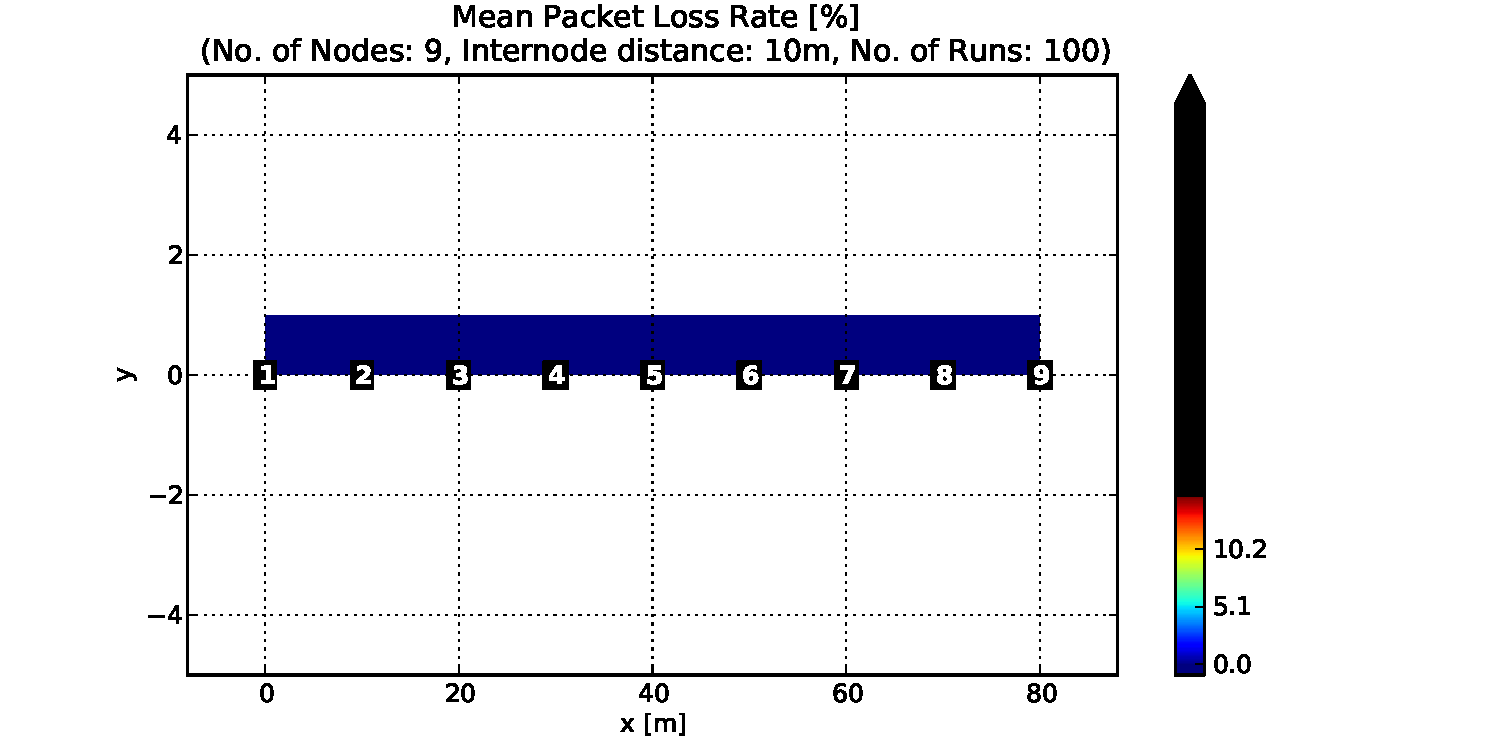
\includegraphics[trim=1.7cm 0cm 3cm 0cm, clip=true, scale=0.38]{Pics/results/9/OF0/line/dist10_montecarlo_contour_packetloss.pdf}}
    \subfloat[MRHOF]{\label{fig:9/MRHOF/line/dist10_montecarlo_contour_packetloss}
      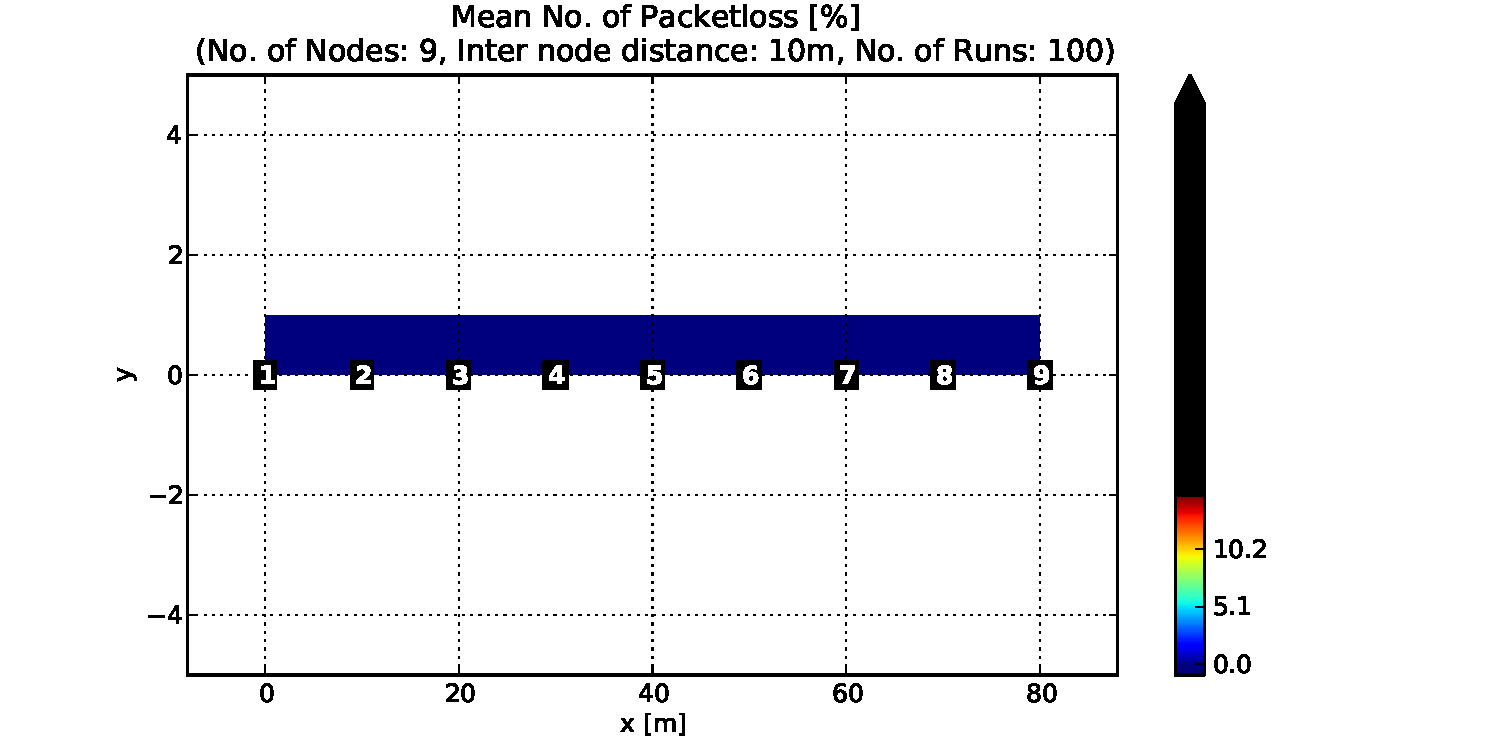
\includegraphics[trim=1.7cm 0cm 3cm 0cm, clip=true, scale=0.38]{Pics/results/9/MRHOF/line/dist10_montecarlo_contour_packetloss.pdf}}
   \caption{Mean packet loss rate: 9-node line scenario with 10 m internode distance}
   \label{fig:pl_9_line_10}
\end{figure}

\begin{figure}[p]
  \centering
    \leavevmode
    \subfloat[OF0]{\label{fig:9/OF0/line/dist50_montecarlo_contour_packetloss}
    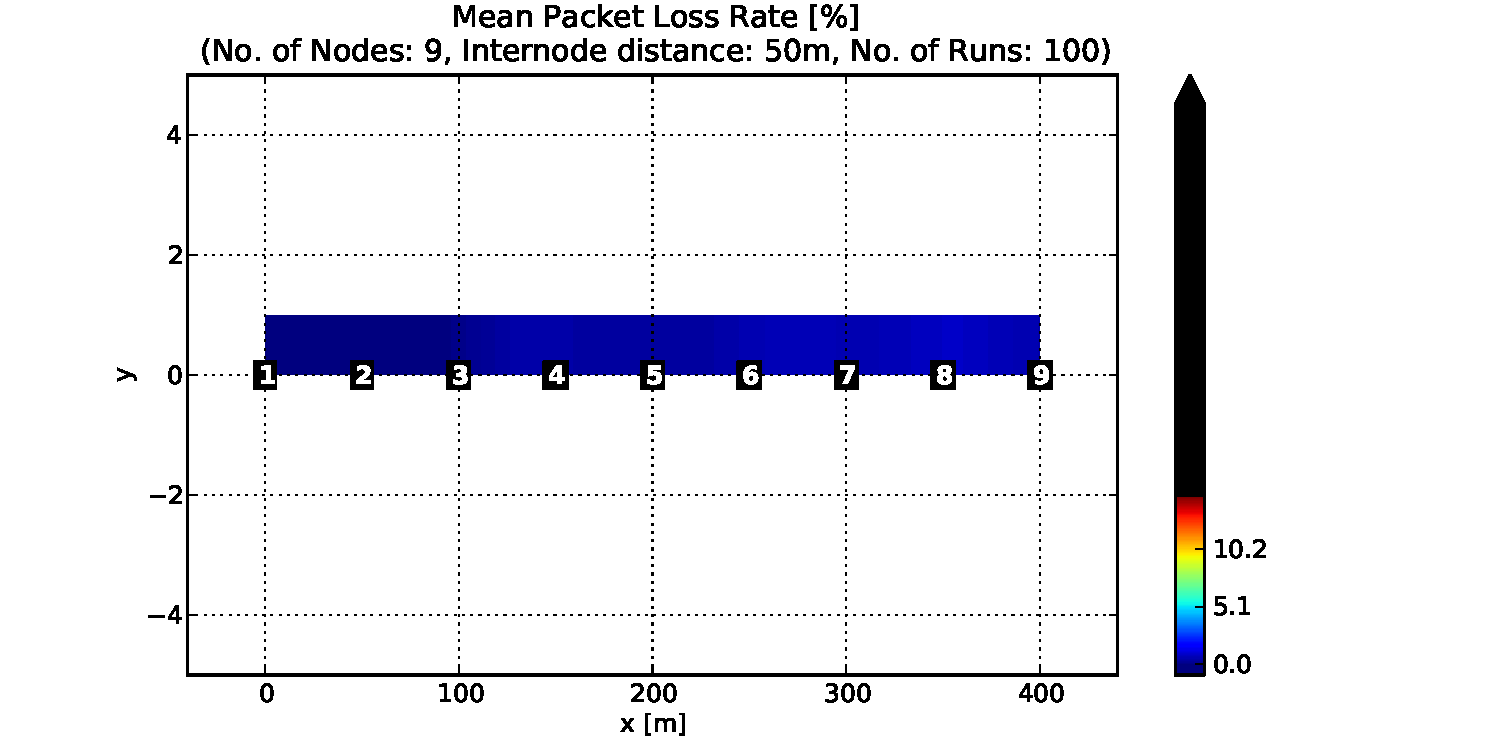
\includegraphics[trim=1.7cm 0cm 3cm 0cm, clip=true, scale=0.38]   {Pics/results/9/OF0/line/dist50_montecarlo_contour_packetloss.pdf}}
    \subfloat[MRHOF]{\label{fig:9/MRHOF/line/dist50_montecarlo_contour_packetloss}
      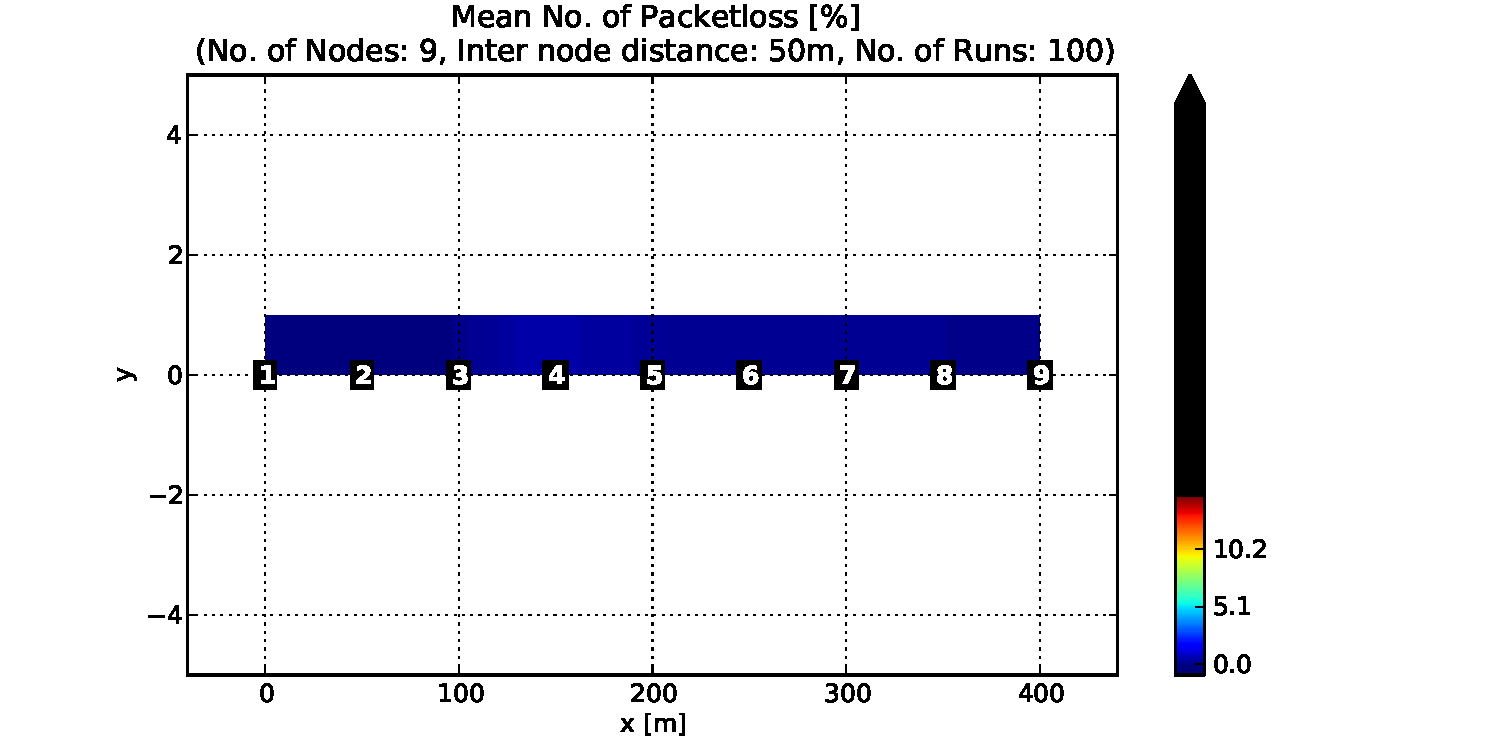
\includegraphics[trim=1.7cm 0cm 3cm 0cm, clip=true, scale=0.38]{Pics/results/9/MRHOF/line/dist50_montecarlo_contour_packetloss.pdf}}
   \caption{Mean packet loss rate: 9-node line scenario with 50 m internode distance}
   \label{fig:pl_9_line_50}
\end{figure}

\begin{figure}[p]
  \centering
    \leavevmode
    \subfloat[OF0]{\label{fig:9/OF0/line/dist100_montecarlo_contour_packetloss}
     \includegraphics[trim=1.7cm 0cm 3cm 0cm, clip=true, scale=0.38]{Pics/results/9/OF0/line/dist100_montecarlo_contour_packetloss.pdf}}
    \subfloat[MRHOF]{\label{fig:9/MRHOF/line/dist100_montecarlo_contour_packetloss}
     \includegraphics[trim=1.7cm 0cm 3cm 0cm, clip=true, scale=0.38]{Pics/results/9/MRHOF/line/dist100_montecarlo_contour_packetloss.pdf}}
  \caption{Mean packet loss rate: 9-node line scenario with 100 m internode distance}
  \label{fig:pl_9_line_100}
\end{figure}

%%%%%%%%%%%%%%%%%%%%%%%%%%%%%%%%%%%%%%% line 16 %%%%%%%%%%%%%%%%%%%%%%%%%%%%%%%%%%%%%%%%

\begin{figure}[p]
  \centering
    \leavevmode
    \subfloat[OF0]{\label{fig:16/OF0/line/dist10_montecarlo_contour_packetloss}
      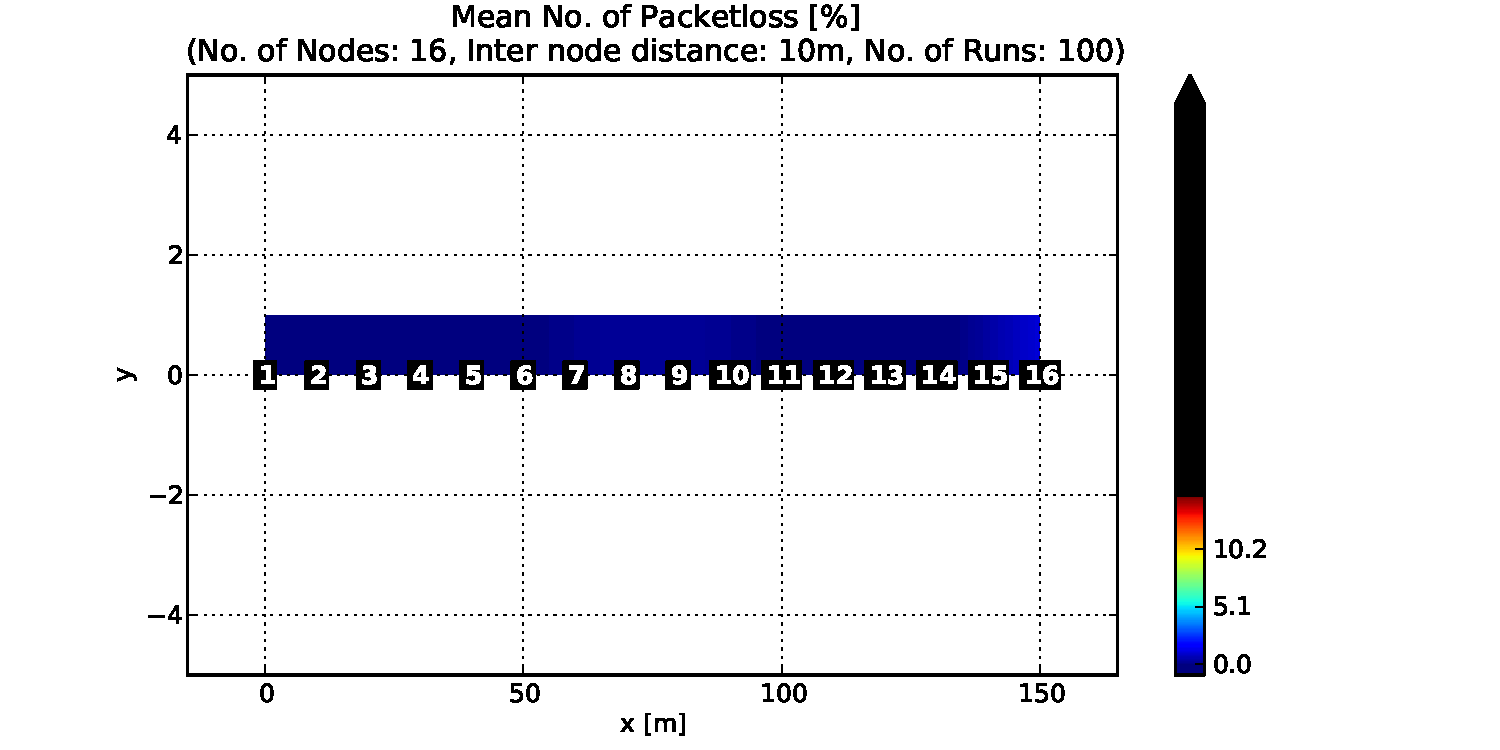
\includegraphics[trim=1.7cm 0cm 3cm 0cm, clip=true, scale=0.38]{Pics/results/16/OF0/line/dist10_montecarlo_contour_packetloss.pdf}}
    \subfloat[MRHOF]{\label{fig:16/MRHOF/line/dist10_montecarlo_contour_packetloss}
      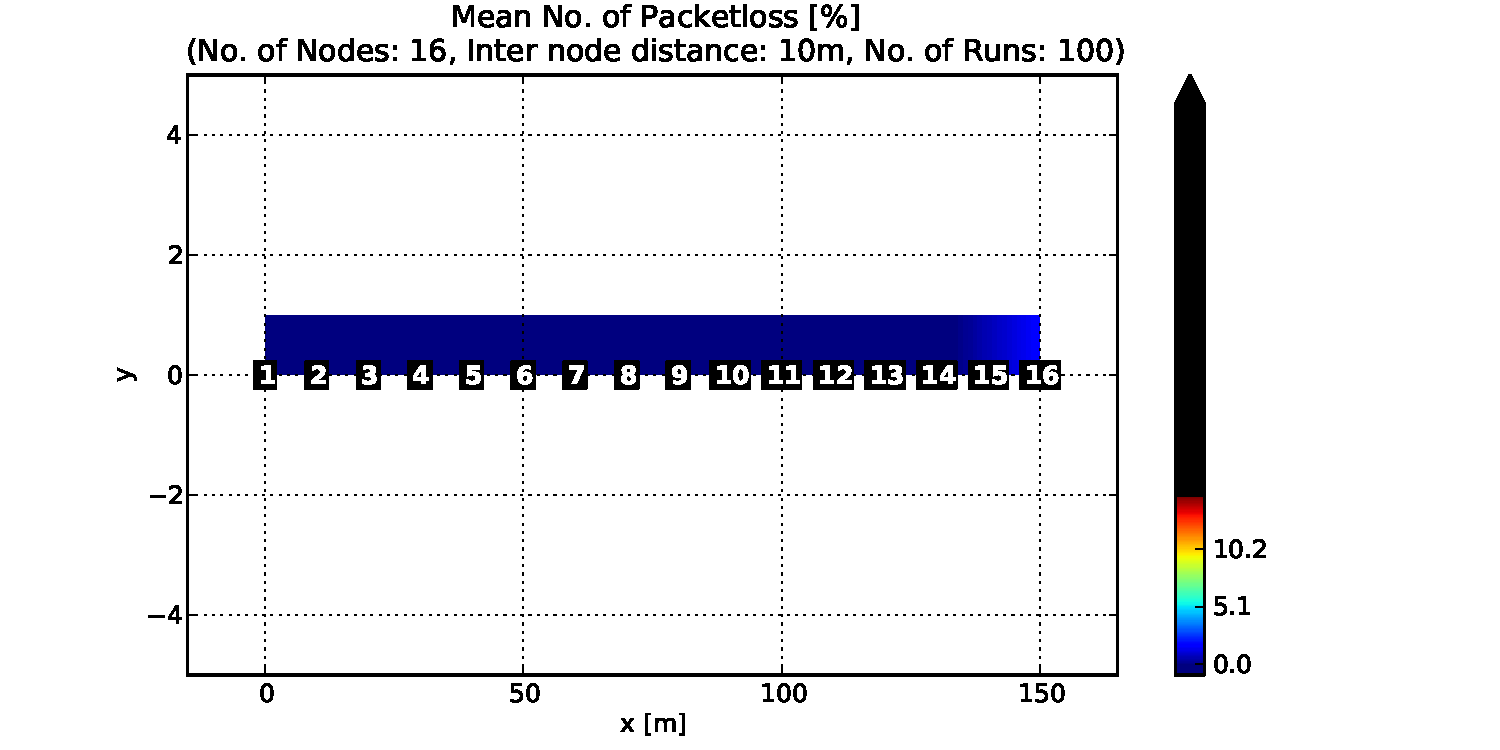
\includegraphics[trim=1.7cm 0cm 3cm 0cm, clip=true, scale=0.38]{Pics/results/16/MRHOF/line/dist10_montecarlo_contour_packetloss.pdf}}
   \caption{Mean packet loss rate: 16-node line scenario with 10 m internode distance}
   \label{fig:pl_16_line_10}
\end{figure}

\begin{figure}[p]
  \centering
    \leavevmode
    \subfloat[OF0]{\label{fig:16/OF0/line/dist50_montecarlo_contour_packetloss}
    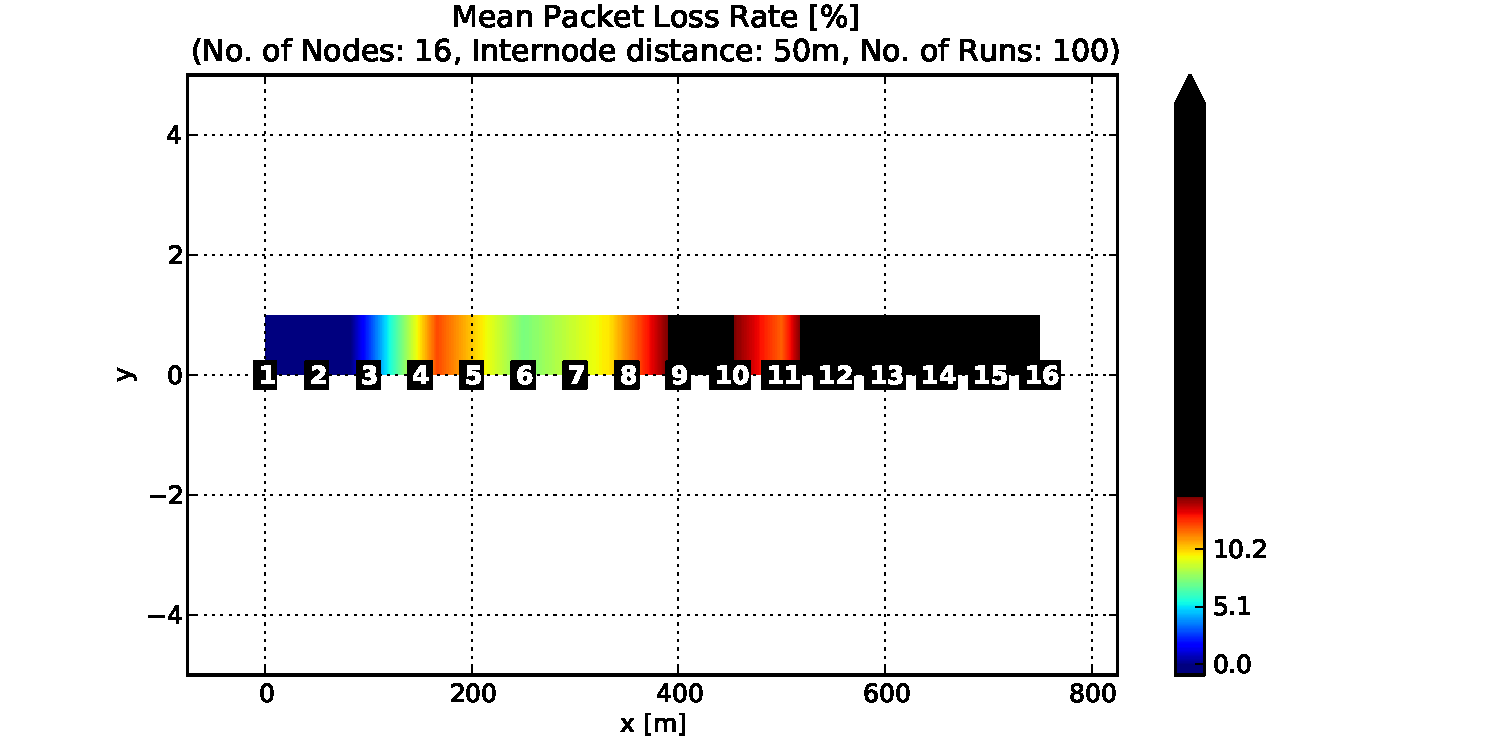
\includegraphics[trim=1.7cm 0cm 3cm 0cm, clip=true, scale=0.38]   {Pics/results/16/OF0/line/dist50_montecarlo_contour_packetloss.pdf}}
    \subfloat[MRHOF]{\label{fig:16/MRHOF/line/dist50_montecarlo_contour_packetloss}
      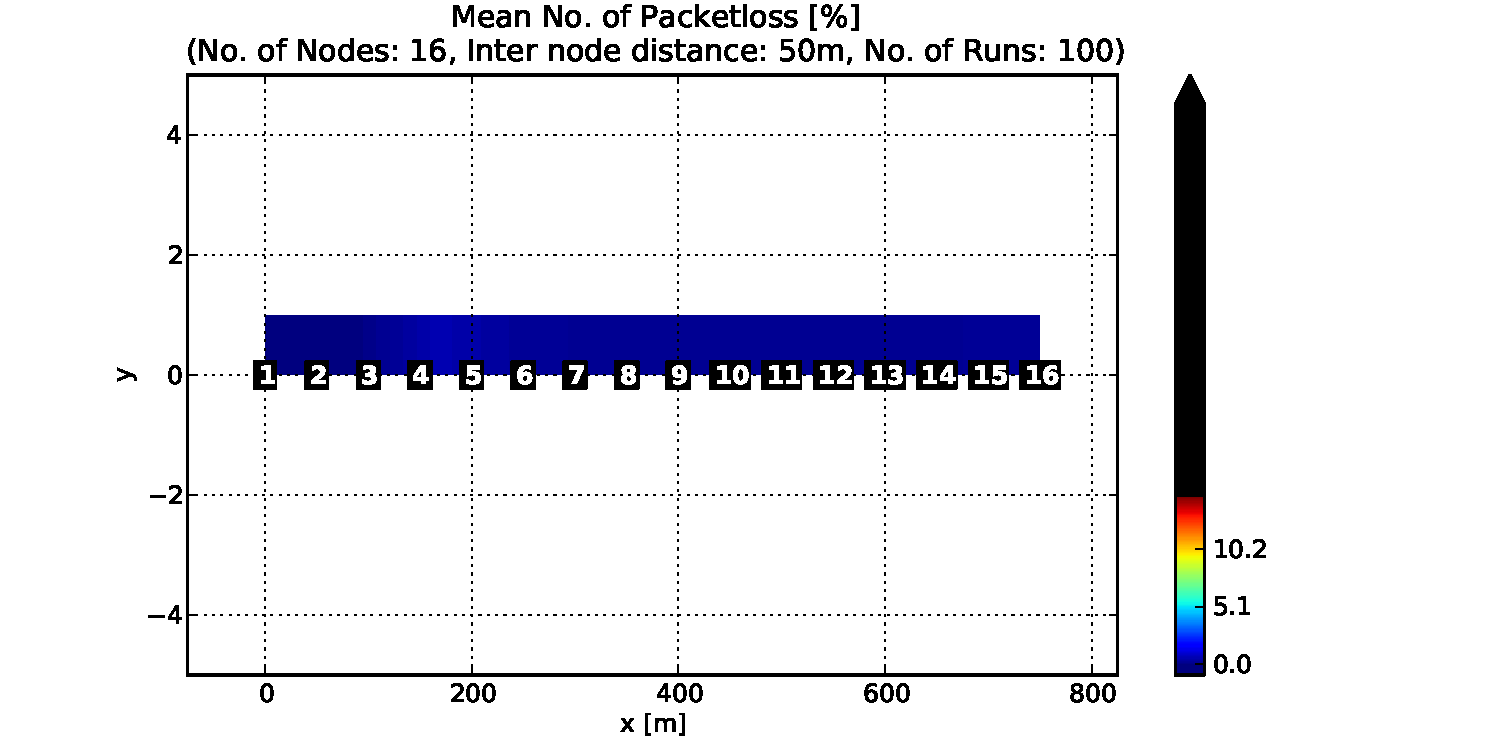
\includegraphics[trim=1.7cm 0cm 3cm 0cm, clip=true, scale=0.38]{Pics/results/16/MRHOF/line/dist50_montecarlo_contour_packetloss.pdf}}
   \caption{Mean packet loss rate: 16-node line scenario with 50 m internode distance}
   \label{fig:pl_16_line_50}
\end{figure}

\begin{figure}[p]
  \centering
    \leavevmode
    \subfloat[OF0]{\label{fig:16/OF0/line/dist100_montecarlo_contour_packetloss}
     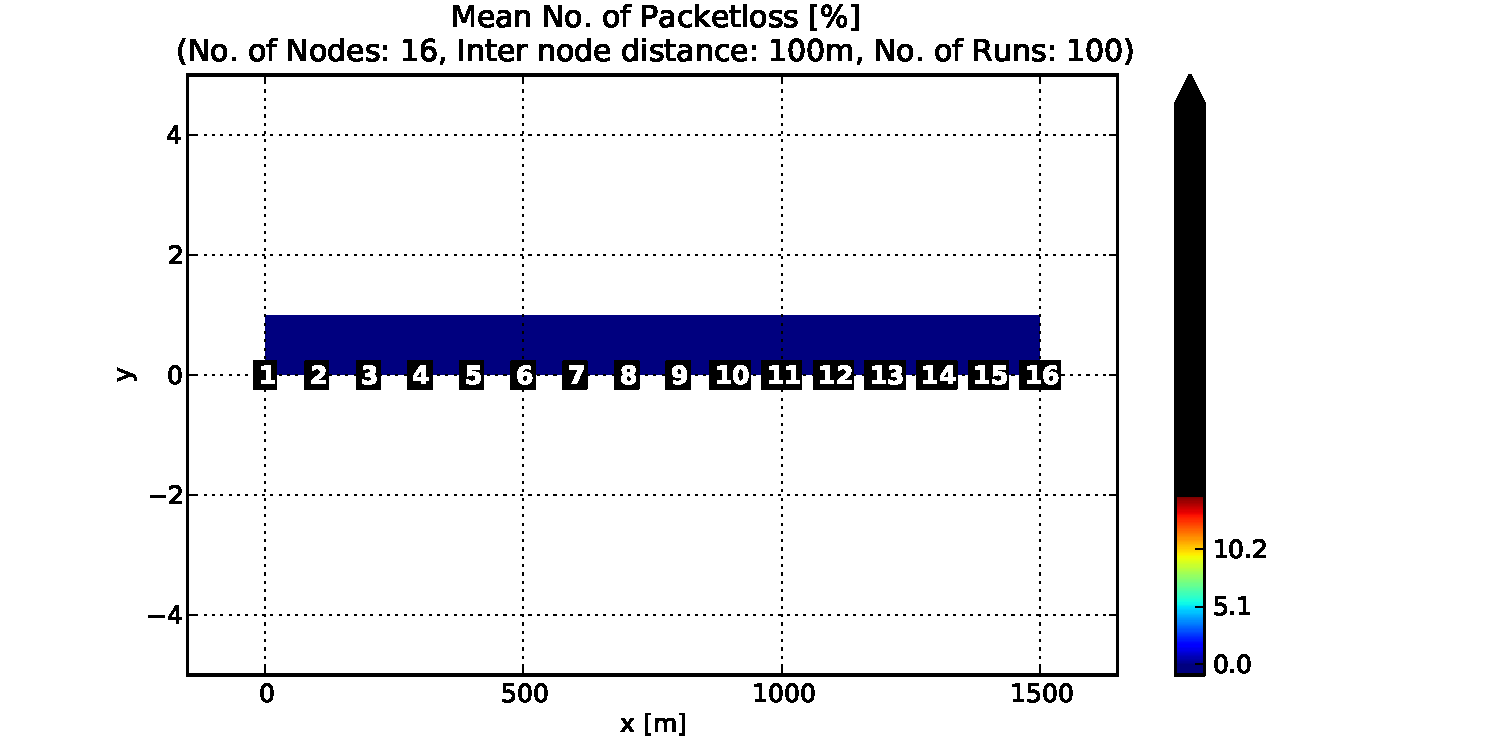
\includegraphics[trim=1.7cm 0cm 3cm 0cm, clip=true, scale=0.38]{Pics/results/16/OF0/line/dist100_montecarlo_contour_packetloss.pdf}}
    \subfloat[MRHOF]{\label{fig:16/MRHOF/line/dist100_montecarlo_contour_packetloss}
     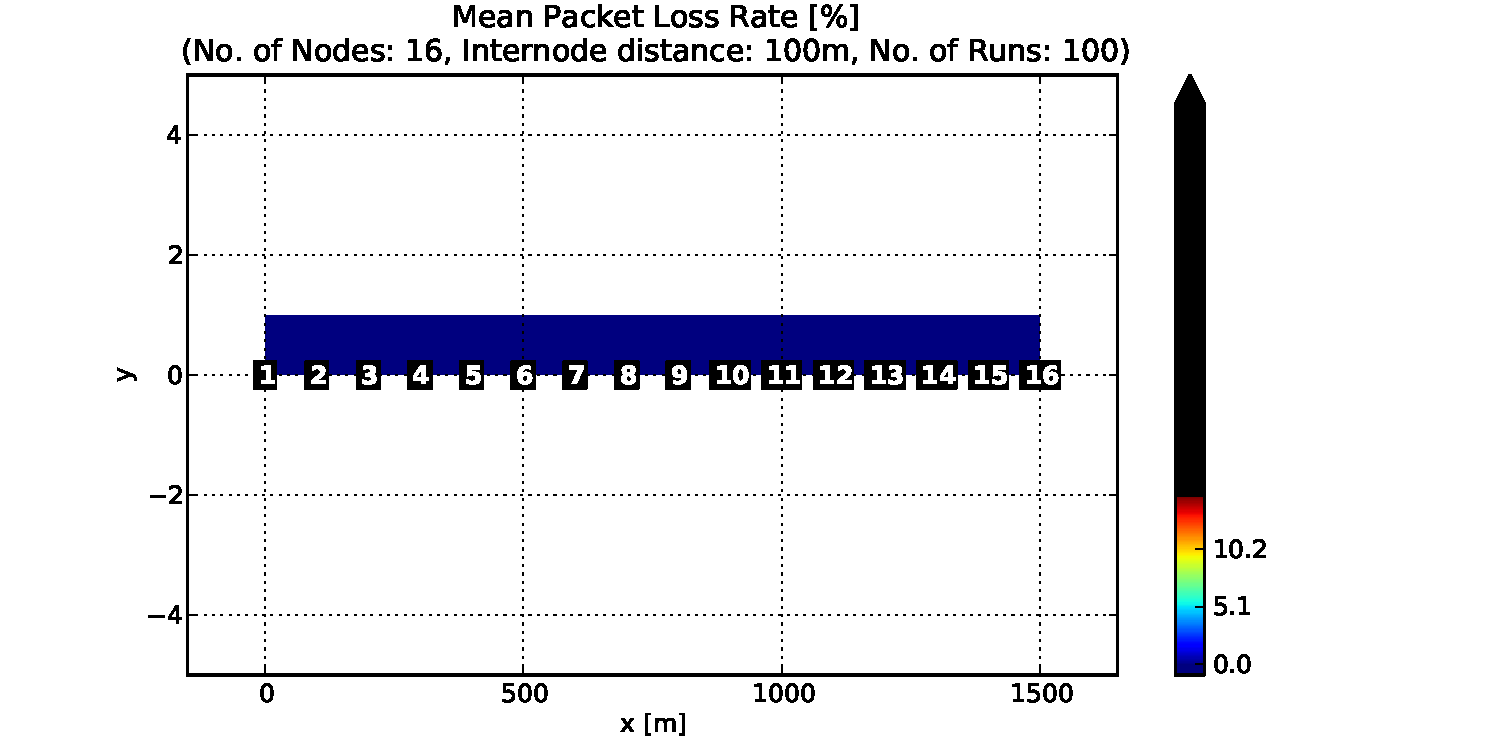
\includegraphics[trim=1.7cm 0cm 3cm 0cm, clip=true, scale=0.38]{Pics/results/16/MRHOF/line/dist100_montecarlo_contour_packetloss.pdf}}
  \caption{Mean packet loss rate: 16-node line scenario with 100 m internode distance}
  \label{fig:pl_16_line_100}
\end{figure}

For the 4-node and 9-node line scenarios, the packet loss under the same setup shows no difference between OF0 and MRHOF. When the node number increases to 16, simulation with OF0 starts to exhibit a higher packet loss than MRHOF. In the 50 meters internode distance case (Figure \ref{fig:16/OF0/line/dist50_montecarlo_contour_packetloss}), one can see a mean packet loss rate higher than 15\% for the most distant nodes. This result is caused either by broken routes, or by a low PRR between the root and the nodes in one or more runs of the 100 runs. When the internode distance increased to 100 meters, OF0 presents again a good case in terms of packet loss rate (Figure \ref{fig:16/OF0/line/dist100_montecarlo_contour_packetloss}). In the meanwhile, MRHOF continues to show a stable result over all runs.   
\newline 

\subsection{Grid Scenario}
\label{pl:grid}
The mean packet loss rate results for grid scenario are shown in Figure \ref{fig:pl_4_grid_10} to Figure \ref{fig:pl_16_grid_100}.

%%%%%%%%%%%%%%%%%%%%%%%%%%%%%%%%%%%%%%% grid 4 %%%%%%%%%%%%%%%%%%%%%%%%%%%%%%%%%%%%%%%%
\begin{figure}[p]
  \centering
    \leavevmode
    \subfloat[OF0]{\label{fig:4/OF0/grid/dist10_montecarlo_contour_packetloss}
      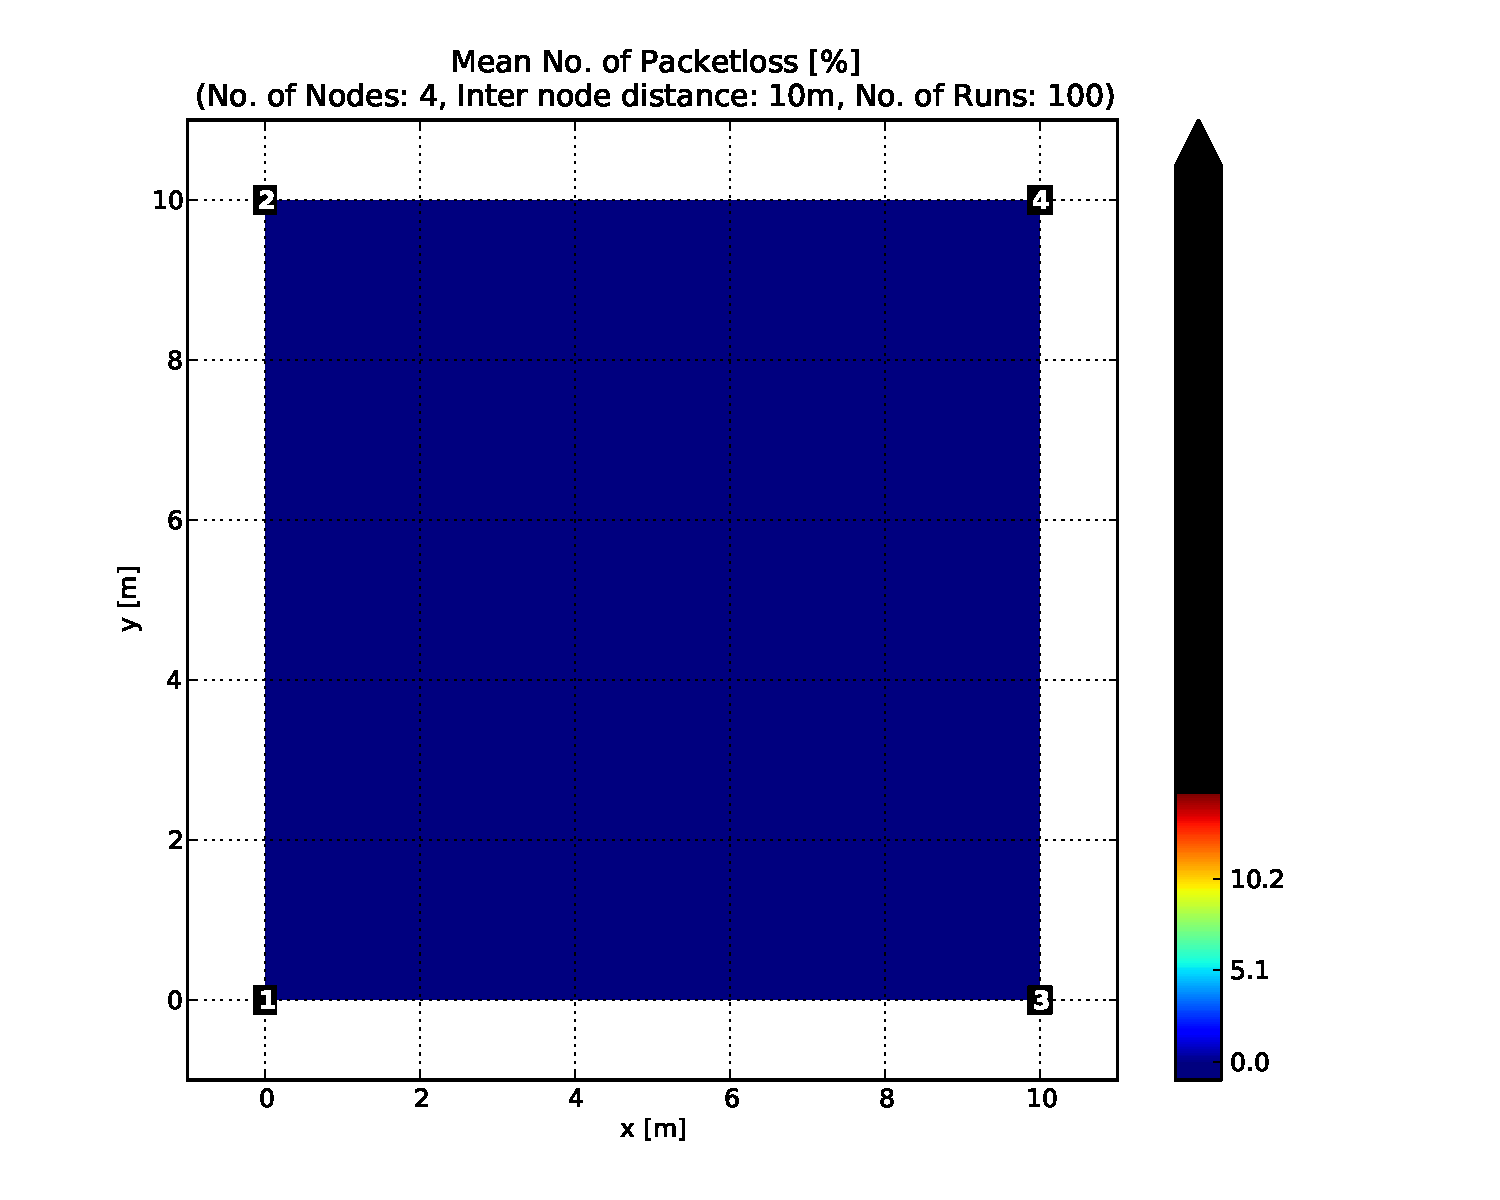
\includegraphics[trim=1.7cm 0cm 3cm 0cm, clip=true, scale=0.38]{Pics/results/4/OF0/grid/dist10_montecarlo_contour_packetloss.pdf}}
    \subfloat[MRHOF]{\label{fig:4/MRHOF/grid/dist10_montecarlo_contour_packetloss}
      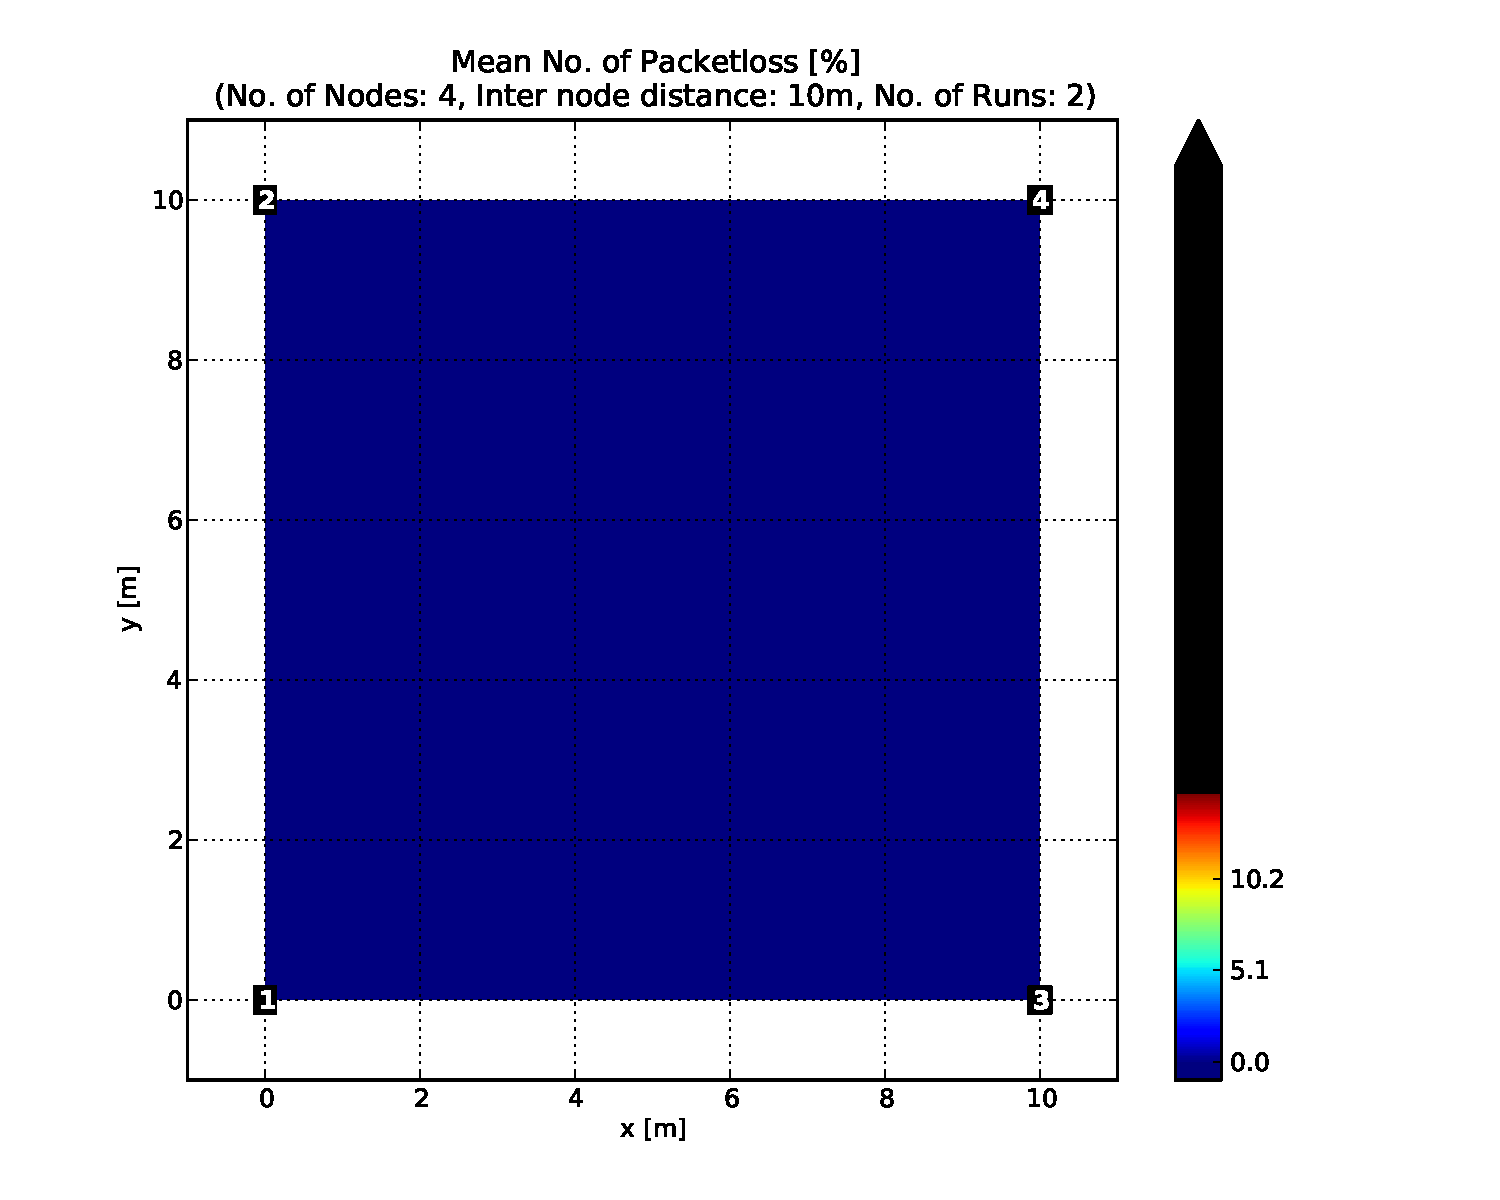
\includegraphics[trim=1.7cm 0cm 3cm 0cm, clip=true, scale=0.38]{Pics/results/4/MRHOF/grid/dist10_montecarlo_contour_packetloss.pdf}}
   \caption{Mean packet loss rate: 4-node grid scenario with 10 m internode distance}
   \label{fig:pl_4_grid_10}
\end{figure}

\begin{figure}[p]
  \centering
    \leavevmode
    \subfloat[OF0]{\label{fig:4/OF0/grid/dist50_montecarlo_contour_packetloss}
    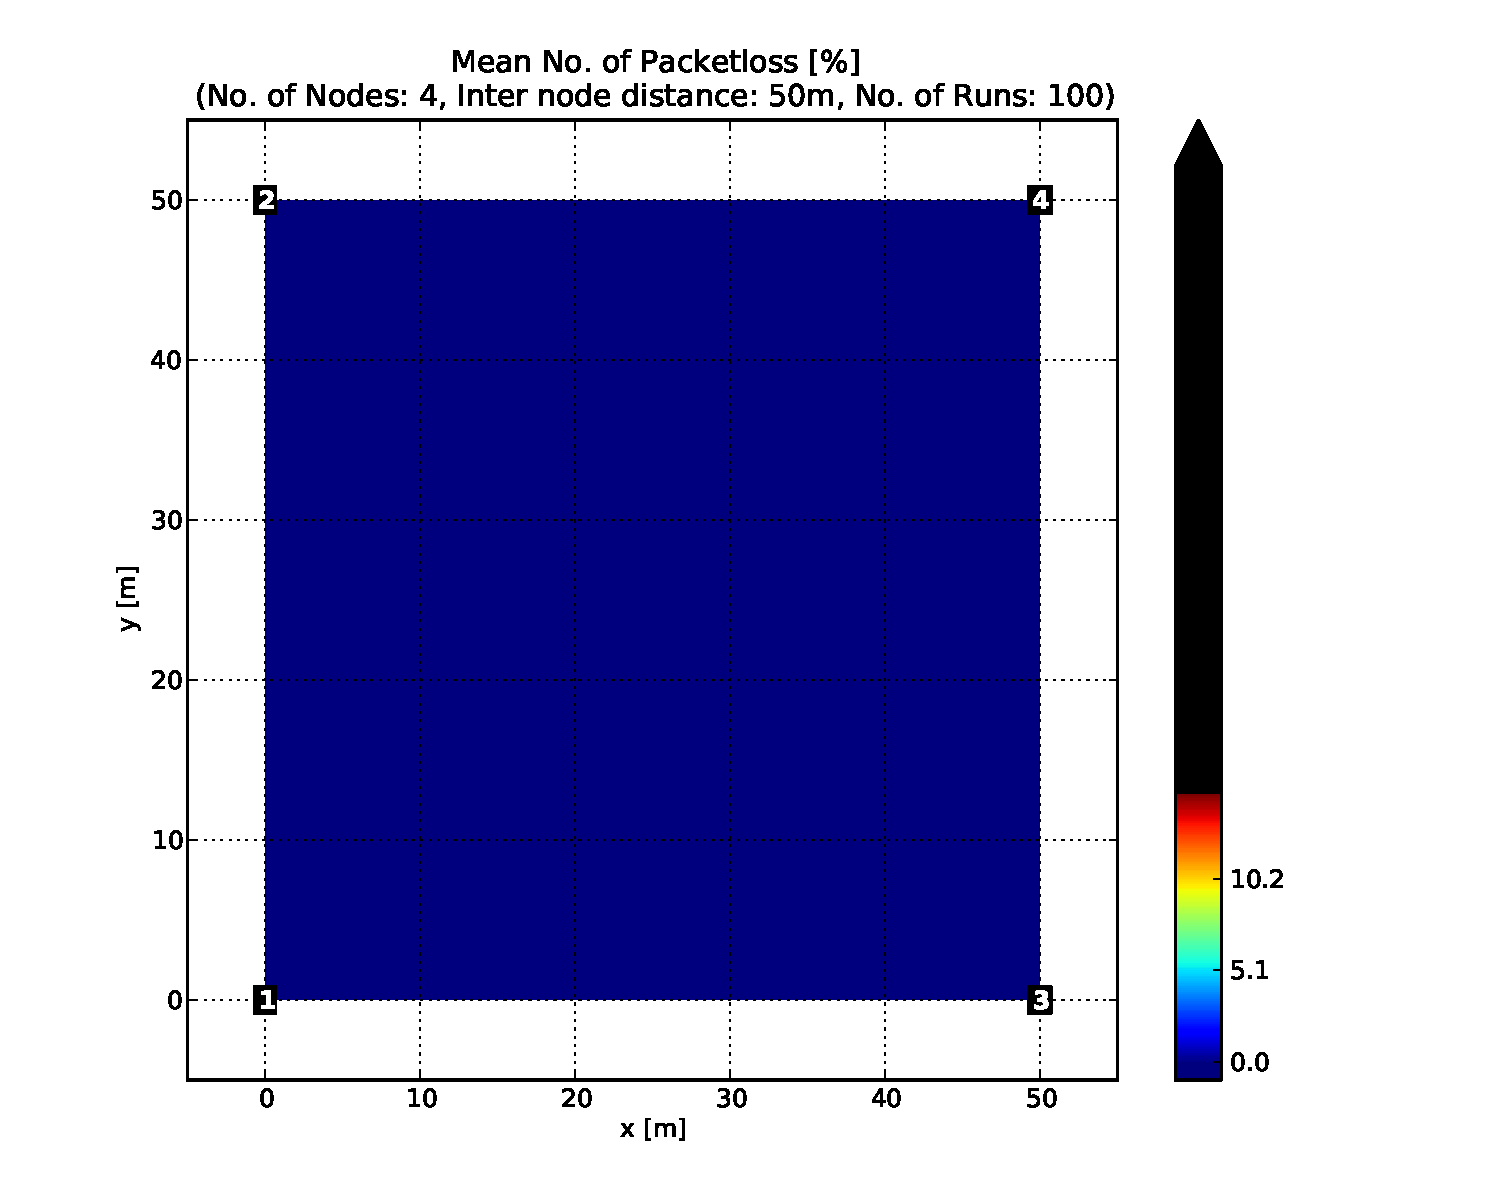
\includegraphics[trim=1.7cm 0cm 3cm 0cm, clip=true, scale=0.38]   {Pics/results/4/OF0/grid/dist50_montecarlo_contour_packetloss.pdf}}
    \subfloat[MRHOF]{\label{fig:4/MRHOF/grid/dist50_montecarlo_contour_packetloss}
      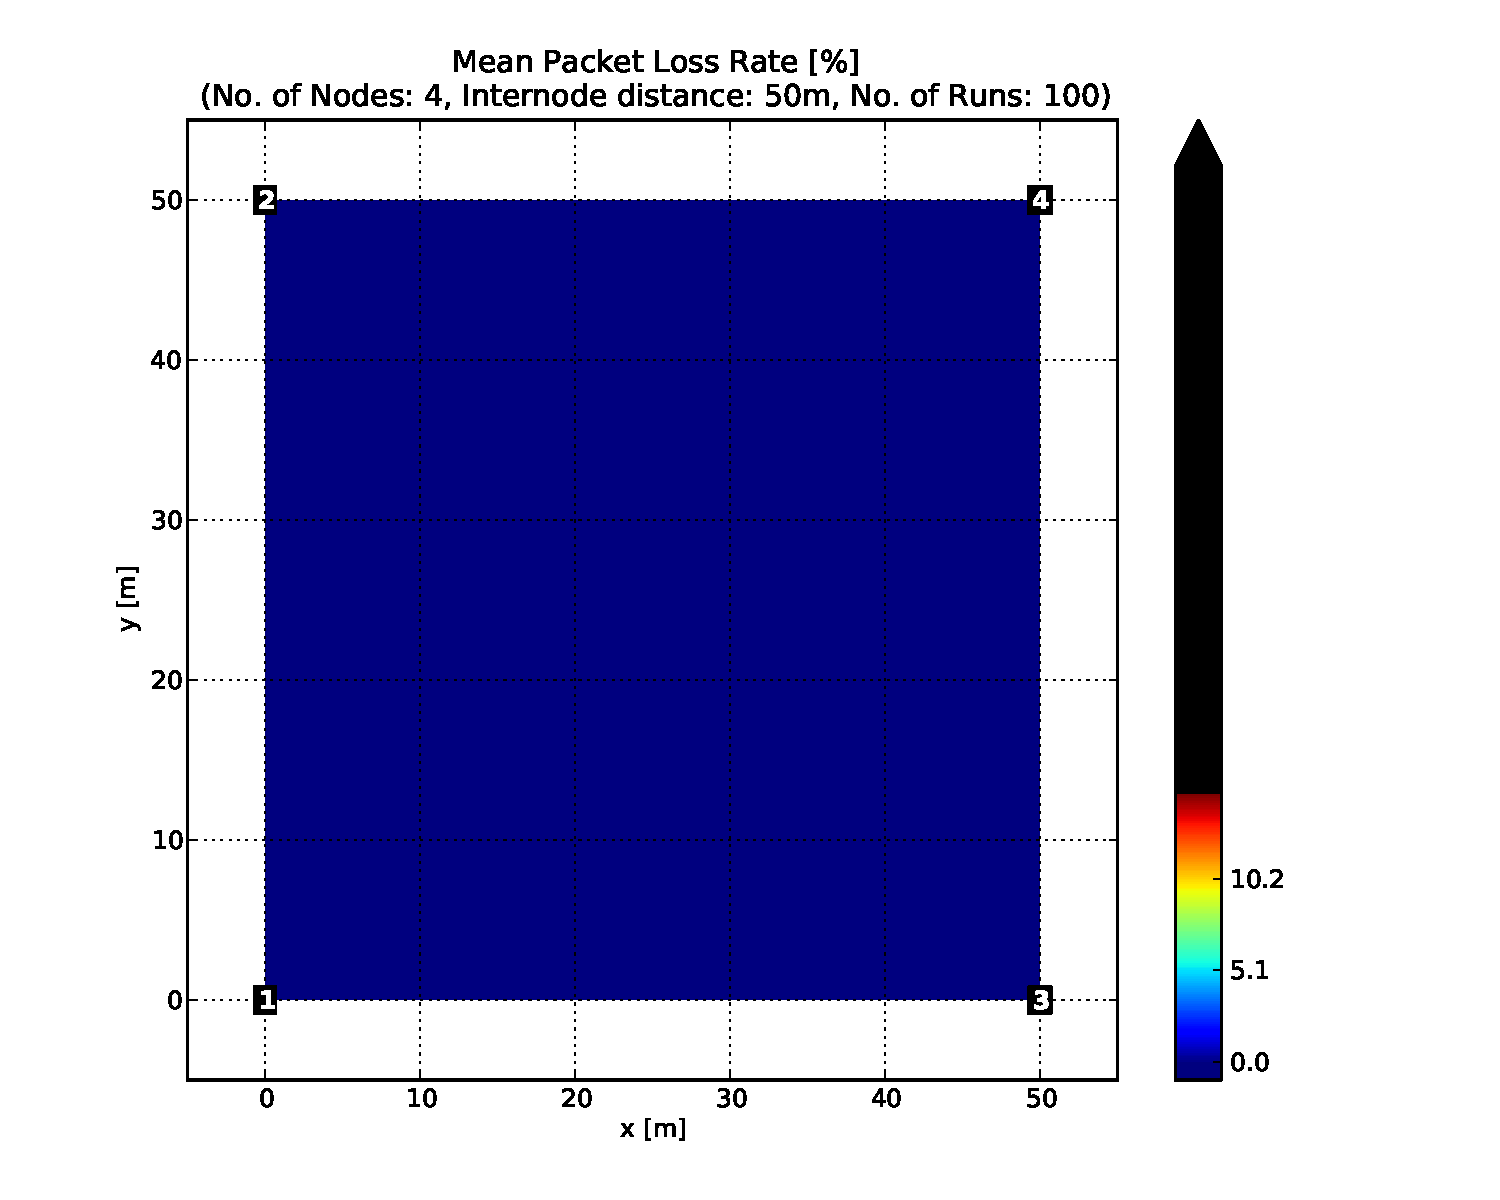
\includegraphics[trim=1.7cm 0cm 3cm 0cm, clip=true, scale=0.38]{Pics/results/4/MRHOF/grid/dist50_montecarlo_contour_packetloss.pdf}}
   \caption{Mean packet loss rate: 4-node grid scenario with 50 m internode distance}
   \label{fig:pl_4_grid_50}
\end{figure}

\begin{figure}[p]
  \centering
    \leavevmode
    \subfloat[OF0]{\label{fig:4/OF0/grid/dist100_montecarlo_contour_packetloss}
     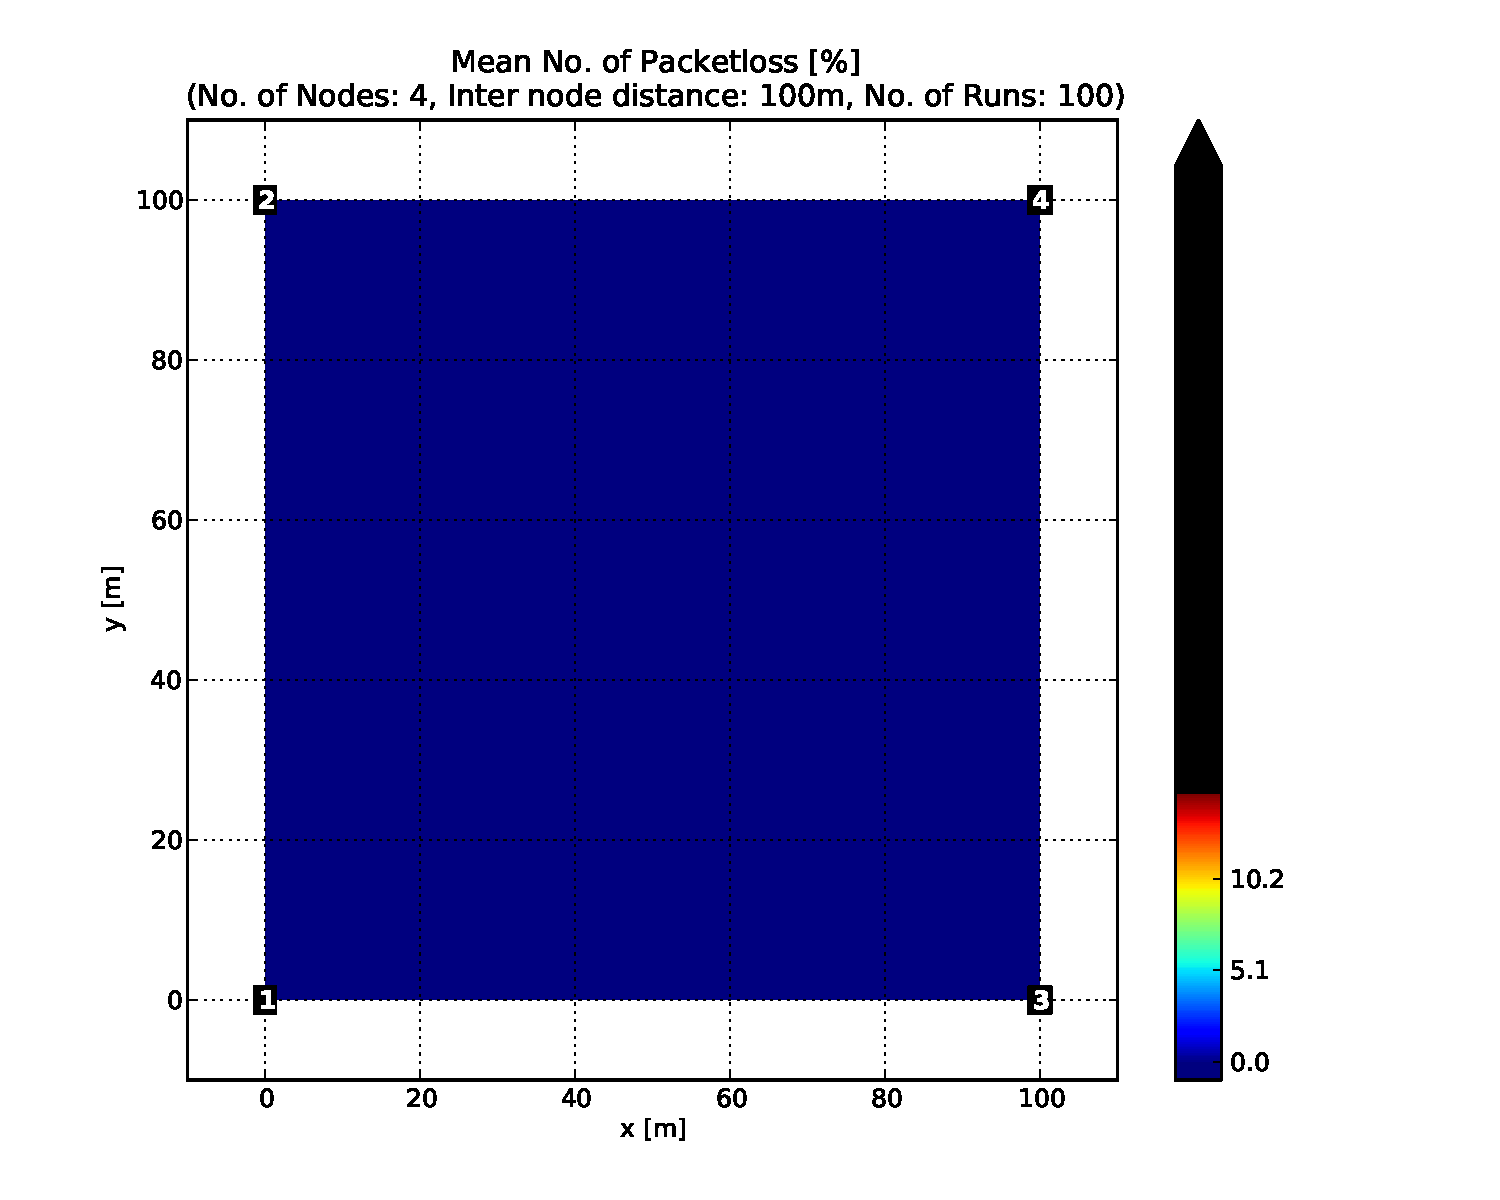
\includegraphics[trim=1.7cm 0cm 3cm 0cm, clip=true, scale=0.38]{Pics/results/4/OF0/grid/dist100_montecarlo_contour_packetloss.pdf}}
    \subfloat[MRHOF]{\label{fig:4/MRHOF/grid/dist100_montecarlo_contour_packetloss}
     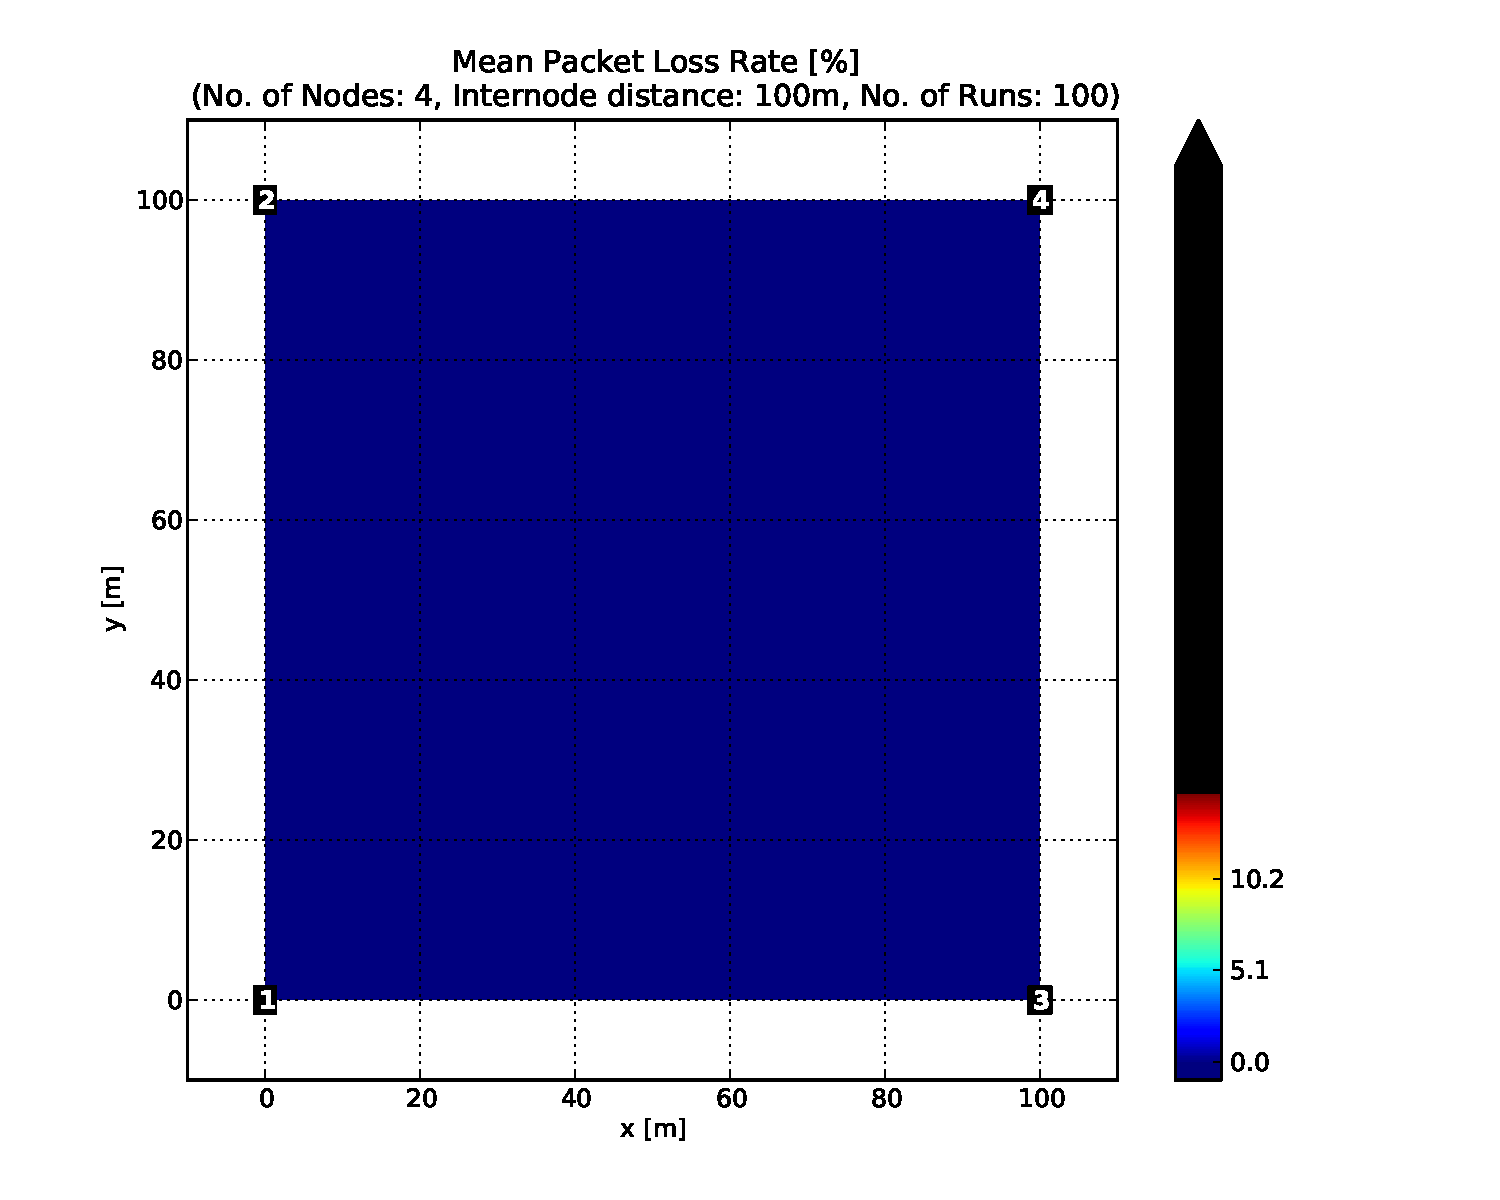
\includegraphics[trim=1.7cm 0cm 3cm 0cm, clip=true, scale=0.38]{Pics/results/4/MRHOF/grid/dist100_montecarlo_contour_packetloss.pdf}}
  \caption{Mean packet loss rate: 4-node grid scenario with 100 m internode distance}
  \label{fig:pl_4_grid_100}
\end{figure}

%%%%%%%%%%%%%%%%%%%%%%%%%%%%%%%%%%%%%%% grid 9 %%%%%%%%%%%%%%%%%%%%%%%%%%%%%%%%%%%%%%%%

\begin{figure}[p]
  \centering
    \leavevmode
    \subfloat[OF0]{\label{fig:9/OF0/grid/dist10_montecarlo_contour_packetloss}
      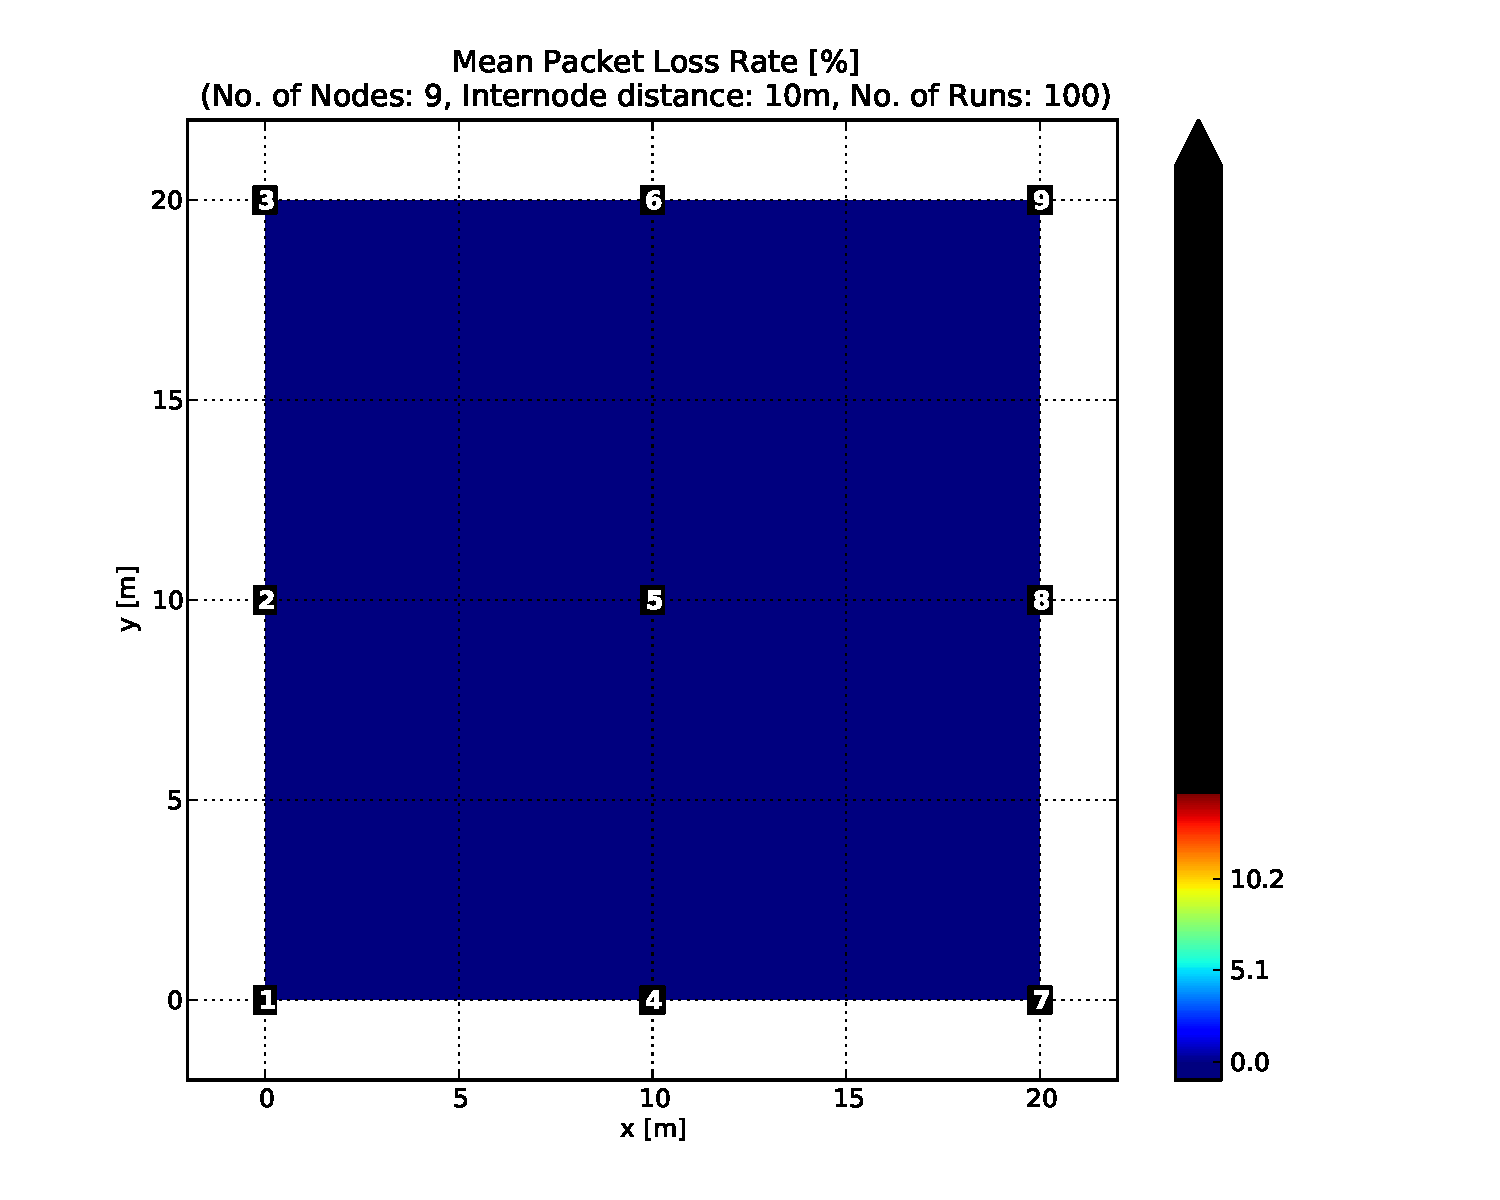
\includegraphics[trim=1.7cm 0cm 3cm 0cm, clip=true, scale=0.38]{Pics/results/9/OF0/grid/dist10_montecarlo_contour_packetloss.pdf}}
    \subfloat[MRHOF]{\label{fig:9/MRHOF/grid/dist10_montecarlo_contour_packetloss}
      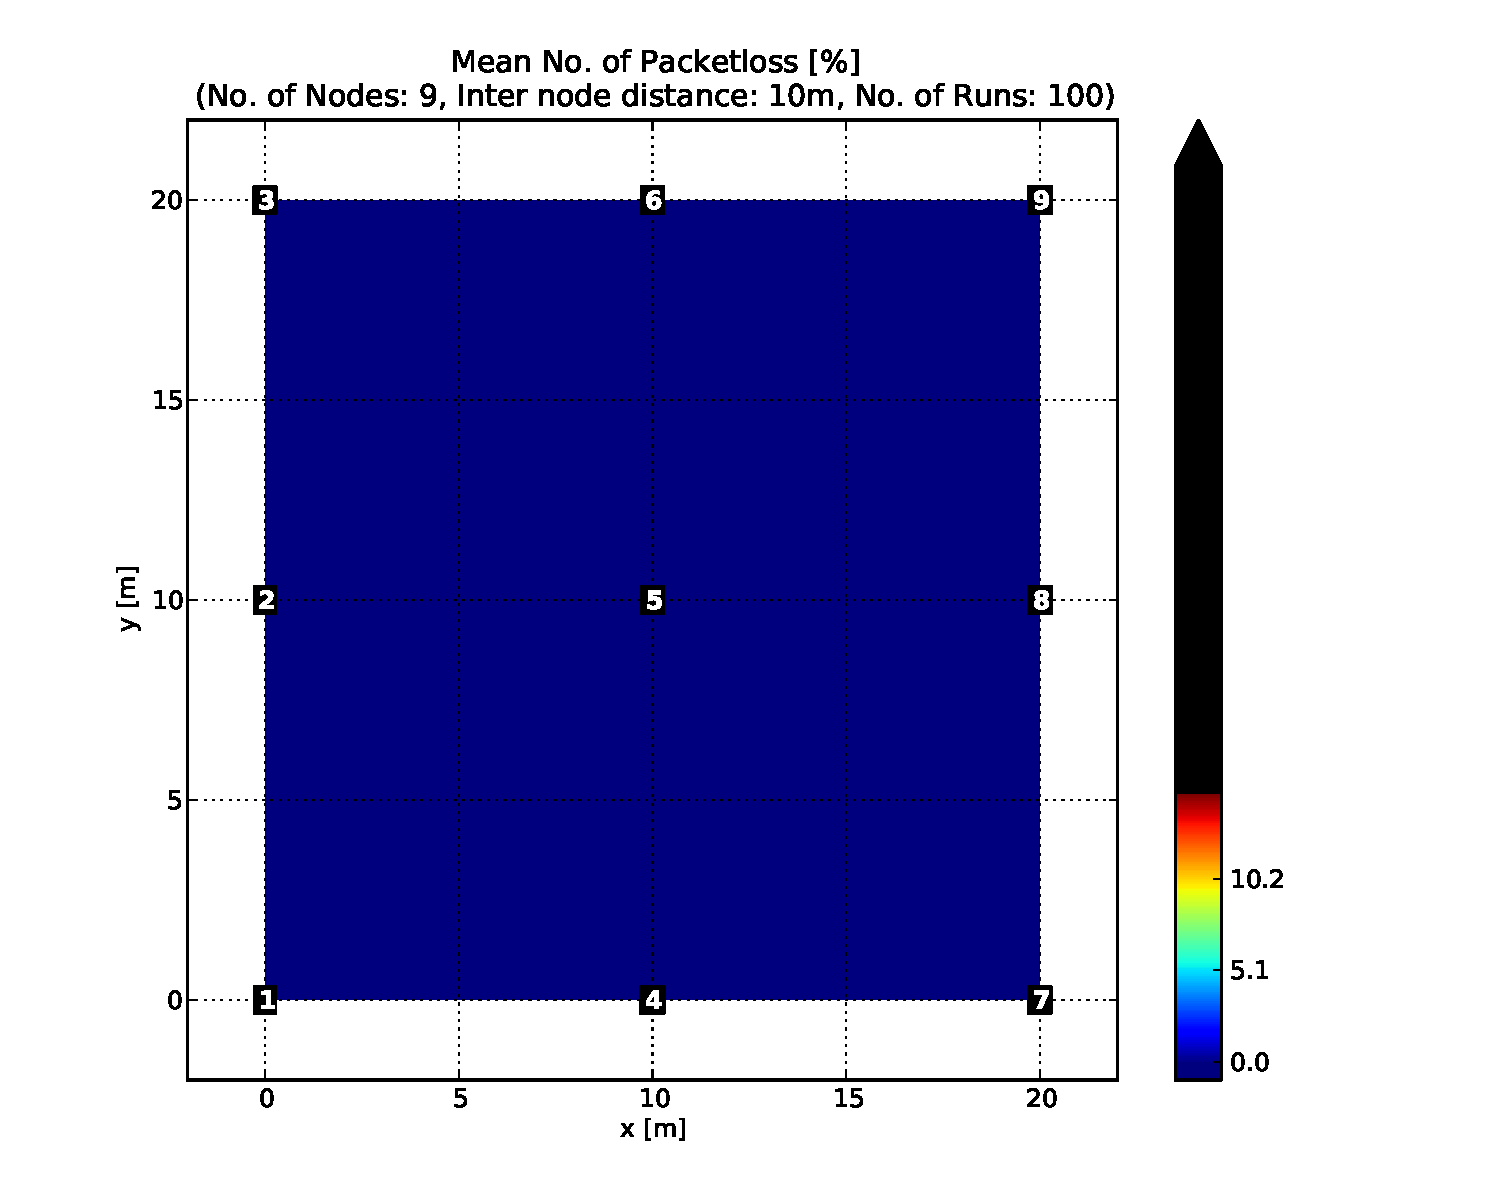
\includegraphics[trim=1.7cm 0cm 3cm 0cm, clip=true, scale=0.38]{Pics/results/9/MRHOF/grid/dist10_montecarlo_contour_packetloss.pdf}}
   \caption{Mean packet loss rate: 9-node grid scenario with 10 m internode distance}
   \label{fig:pl_9_grid_10}
\end{figure}

\begin{figure}[p]
  \centering
    \leavevmode
    \subfloat[OF0]{\label{fig:9/OF0/grid/dist50_montecarlo_contour_packetloss}
    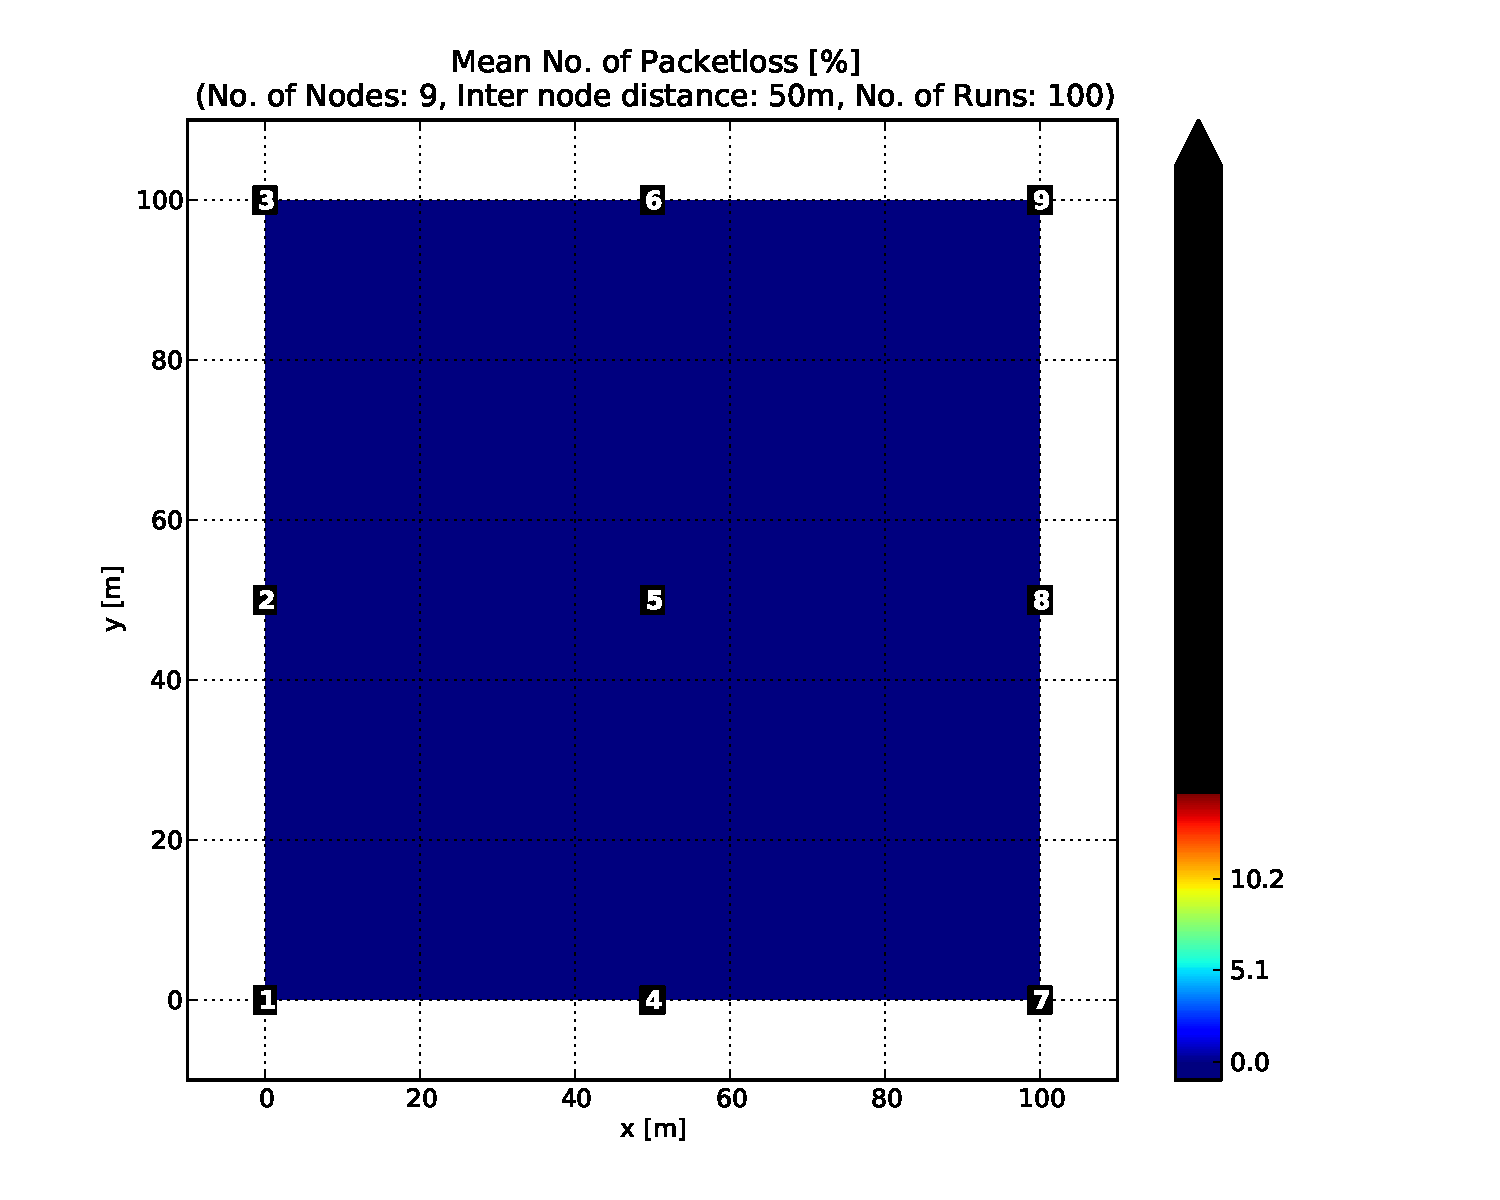
\includegraphics[trim=1.7cm 0cm 3cm 0cm, clip=true, scale=0.38]   {Pics/results/9/OF0/grid/dist50_montecarlo_contour_packetloss.pdf}}
    \subfloat[MRHOF]{\label{fig:9/MRHOF/grid/dist50_montecarlo_contour_packetloss}
      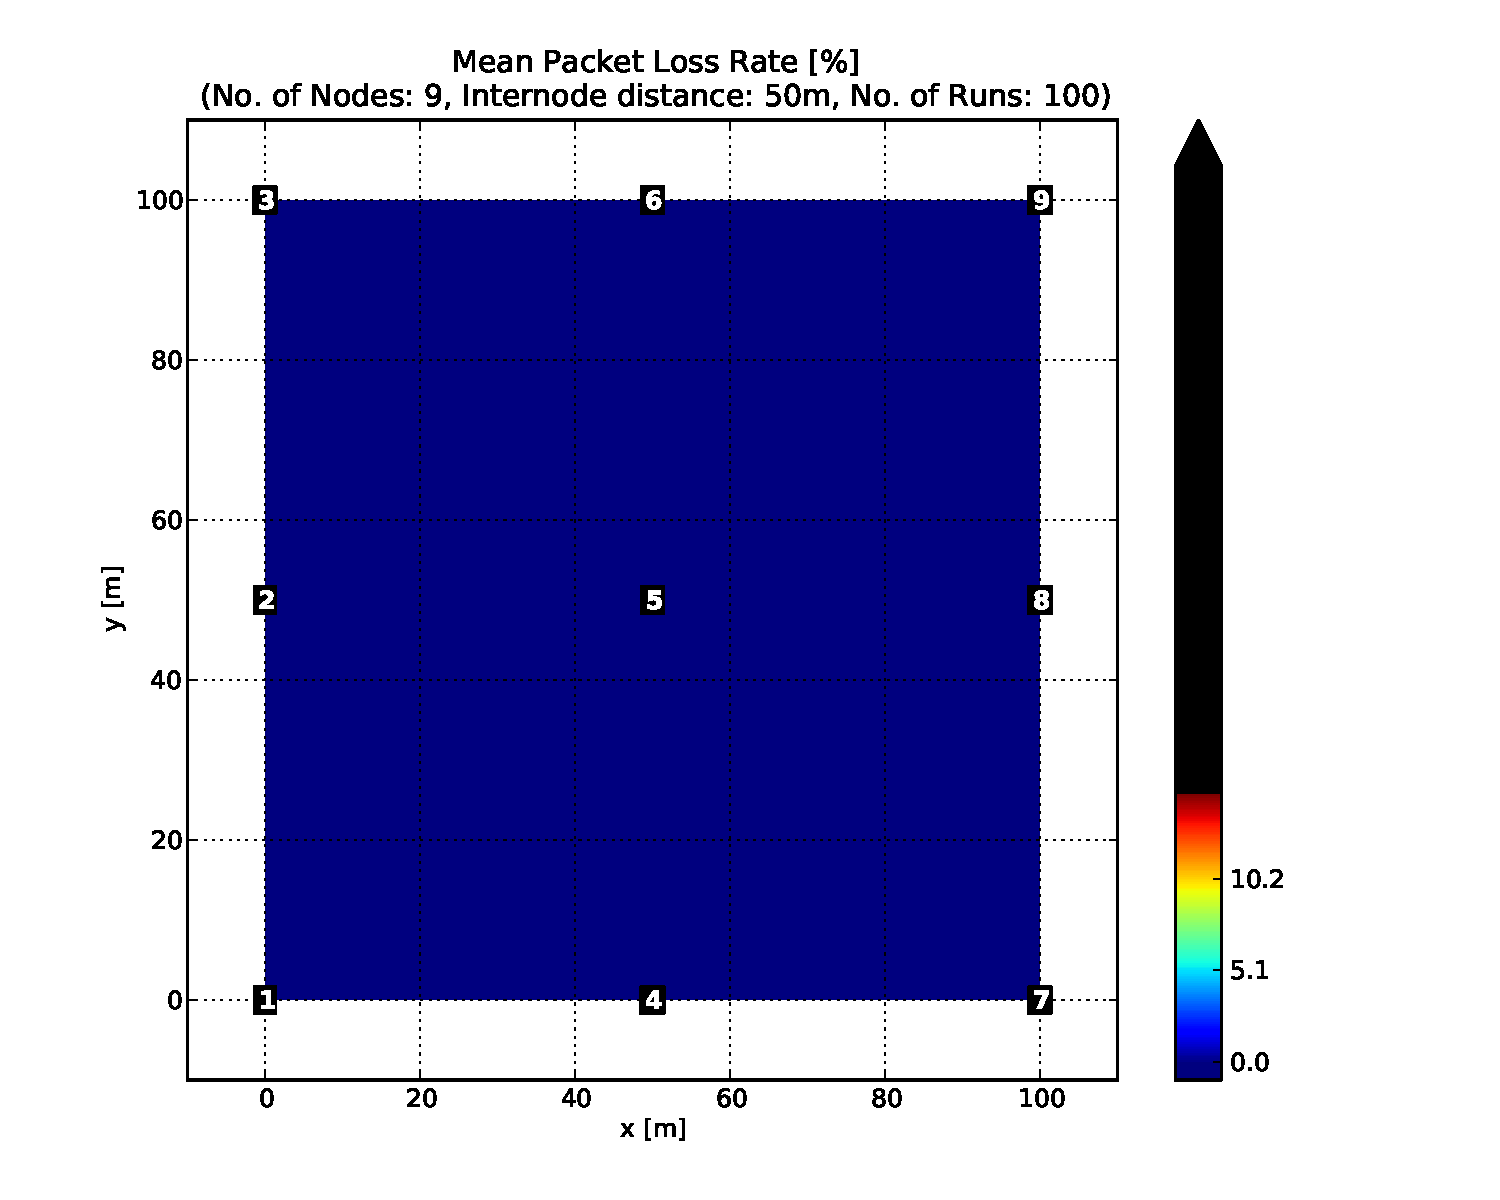
\includegraphics[trim=1.7cm 0cm 3cm 0cm, clip=true, scale=0.38]{Pics/results/9/MRHOF/grid/dist50_montecarlo_contour_packetloss.pdf}}
   \caption{Mean packet loss rate: 9-node grid scenario with 50 m internode distance}
   \label{fig:pl_9_grid_50}
\end{figure}

\begin{figure}[p]
  \centering
    \leavevmode
    \subfloat[OF0]{\label{fig:9/OF0/grid/dist100_montecarlo_contour_packetloss}
     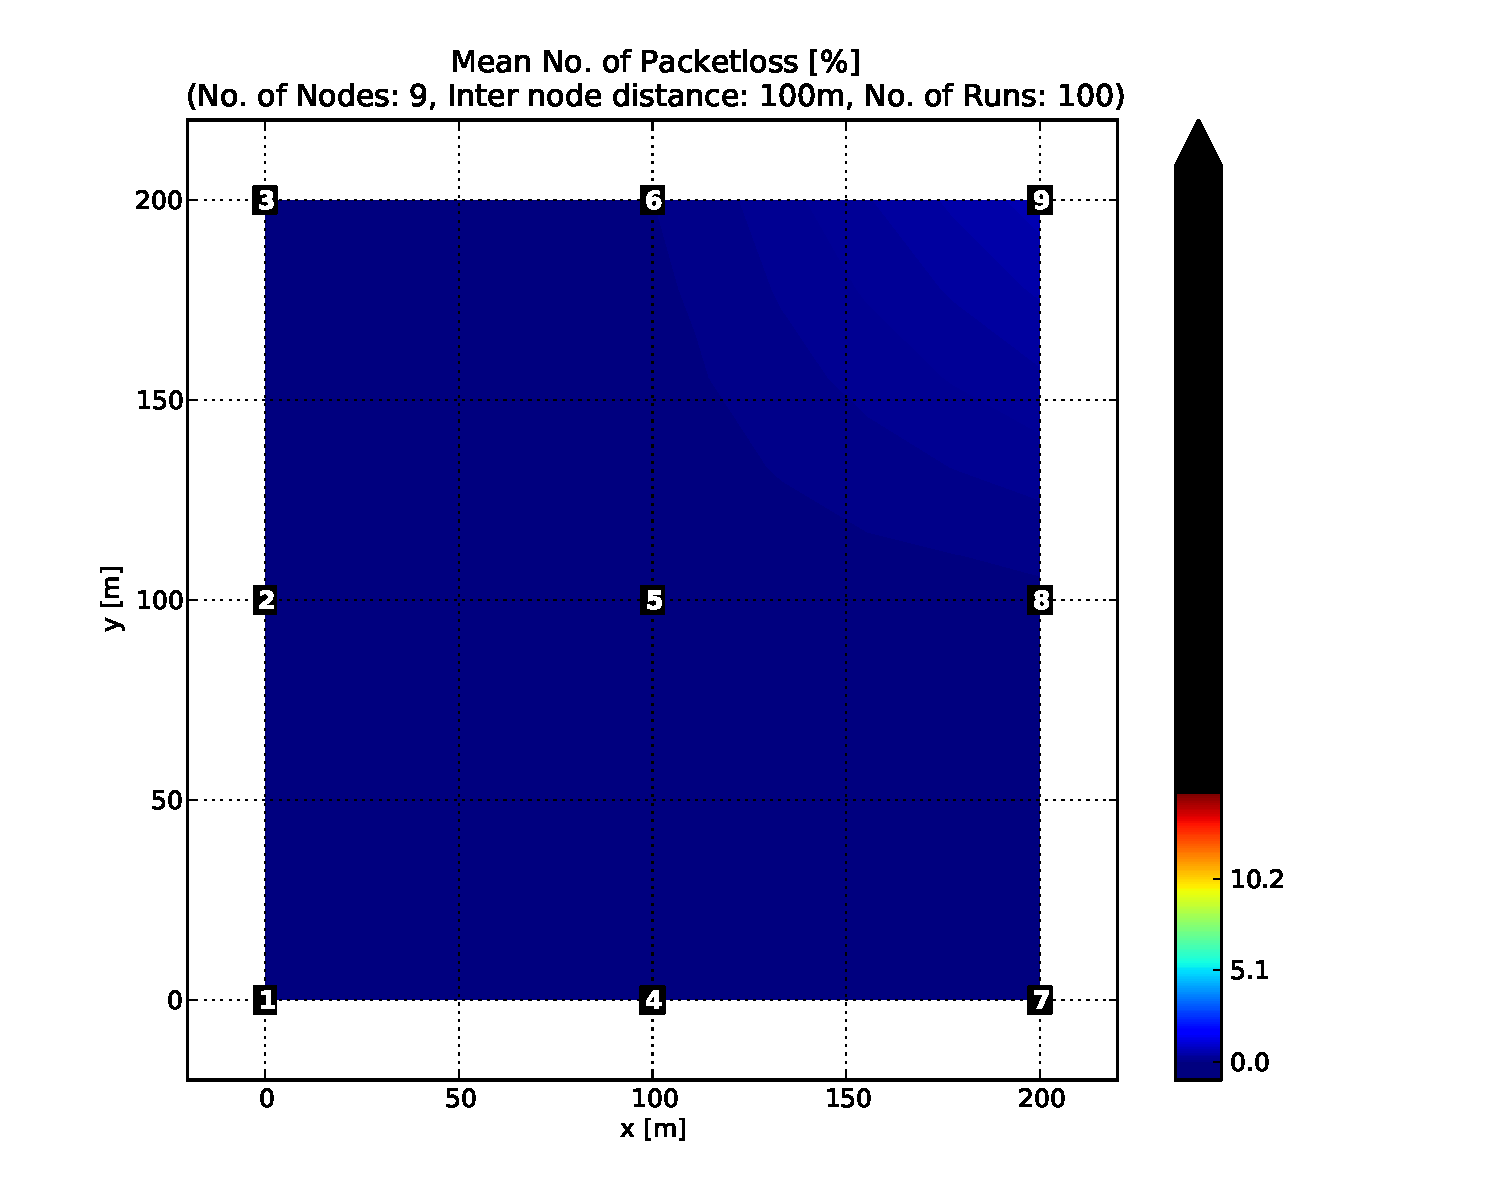
\includegraphics[trim=1.7cm 0cm 3cm 0cm, clip=true, scale=0.38]{Pics/results/9/OF0/grid/dist100_montecarlo_contour_packetloss.pdf}}
    \subfloat[MRHOF]{\label{fig:9/MRHOF/grid/dist100_montecarlo_contour_packetloss}
     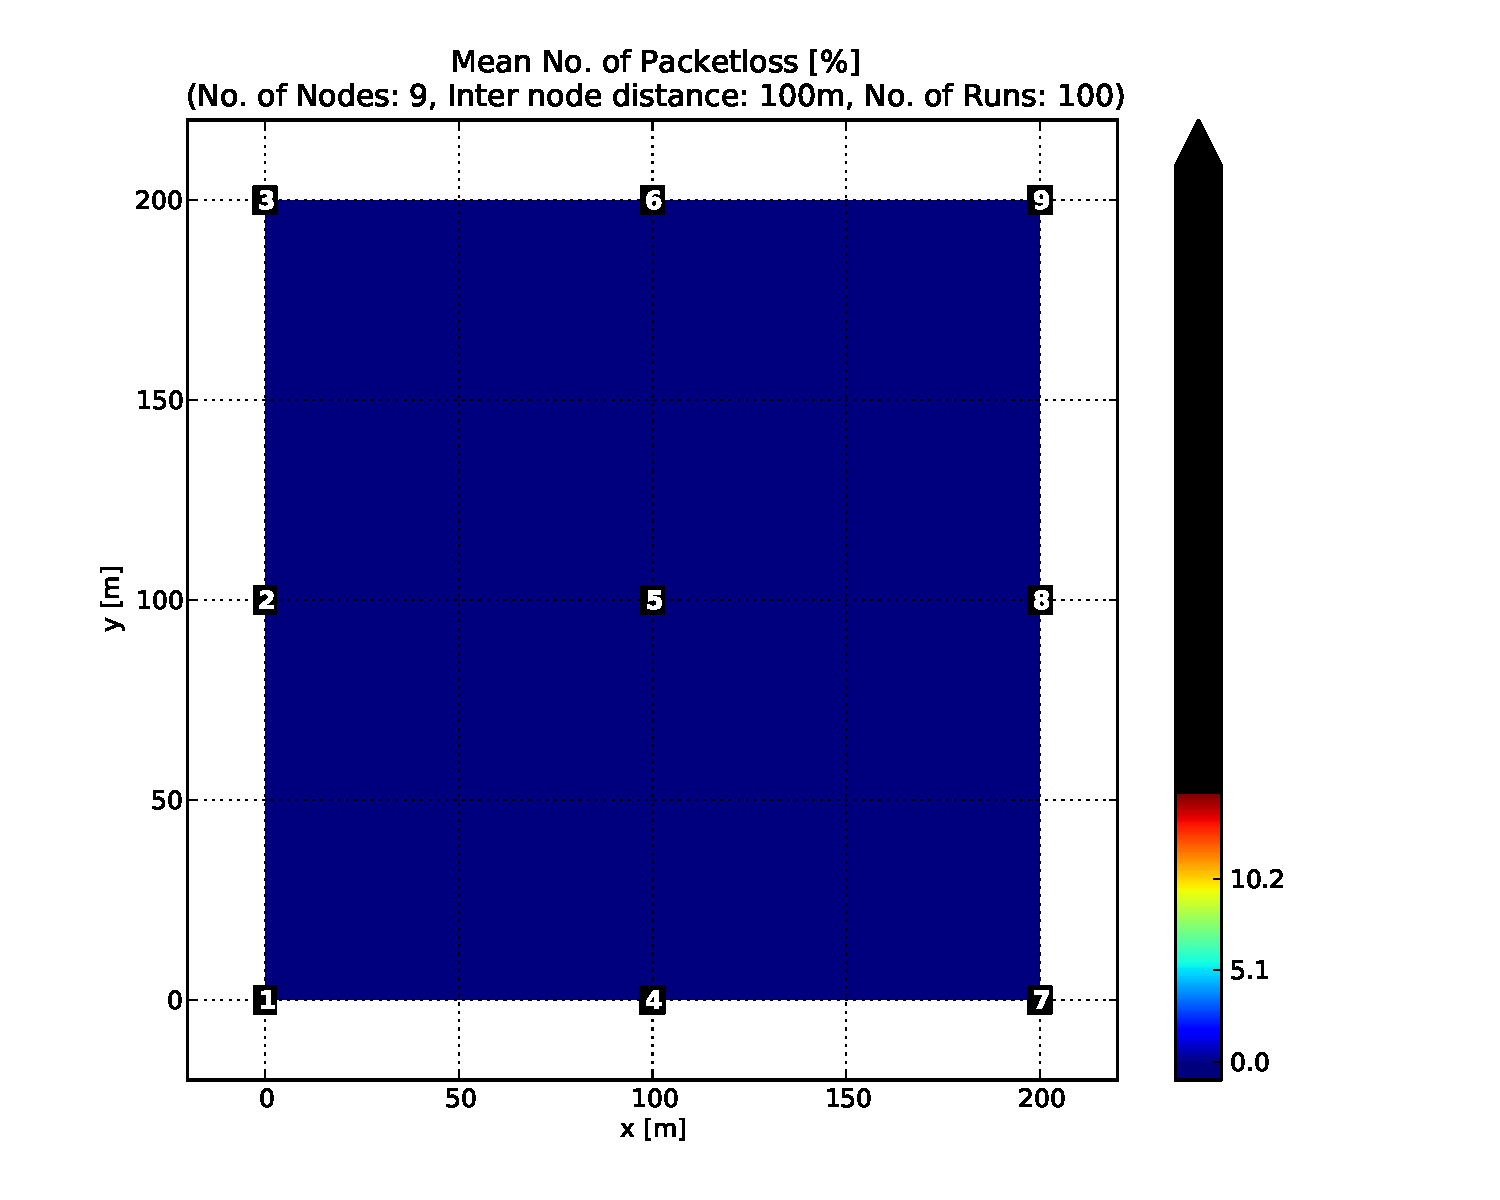
\includegraphics[trim=1.7cm 0cm 3cm 0cm, clip=true, scale=0.38]{Pics/results/9/MRHOF/grid/dist100_montecarlo_contour_packetloss.pdf}}
  \caption{Mean packet loss rate: 9-node grid scenario with 100 m internode distance}
  \label{fig:pl_9_grid_100}
\end{figure}

%%%%%%%%%%%%%%%%%%%%%%%%%%%%%%%%%%%%%%% grid 16 %%%%%%%%%%%%%%%%%%%%%%%%%%%%%%%%%%%%%%%%

\begin{figure}[p]
  \centering
    \leavevmode
    \subfloat[OF0]{\label{fig:16/OF0/grid/dist10_montecarlo_contour_packetloss}
      \includegraphics[trim=1.7cm 0cm 3cm 0cm, clip=true, scale=0.38]{Pics/results/16/OF0/grid/dist10_montecarlo_contour_packetloss.pdf}}
    \subfloat[MRHOF]{\label{fig:16/MRHOF/grid/dist10_montecarlo_contour_packetloss}
      \includegraphics[trim=1.7cm 0cm 3cm 0cm, clip=true, scale=0.38]{Pics/results/16/MRHOF/grid/dist10_montecarlo_contour_packetloss.pdf}}
   \caption{Mean packet loss rate: 16-node grid scenario with 10 m internode distance}
   \label{fig:pl_16_grid_10}
\end{figure}

\begin{figure}[p]
  \centering
    \leavevmode
    \subfloat[OF0]{\label{fig:16/OF0/grid/dist50_montecarlo_contour_packetloss}
    \includegraphics[trim=1.7cm 0cm 3cm 0cm, clip=true, scale=0.38]   {Pics/results/16/OF0/grid/dist50_montecarlo_contour_packetloss.pdf}}
    \subfloat[MRHOF]{\label{fig:16/MRHOF/grid/dist50_montecarlo_contour_packetloss}
      \includegraphics[trim=1.7cm 0cm 3cm 0cm, clip=true, scale=0.38]{Pics/results/16/MRHOF/grid/dist50_montecarlo_contour_packetloss.pdf}}
   \caption{Mean packet loss rate: 16-node grid scenario with 50 m internode distance}
   \label{fig:pl_16_grid_50}
\end{figure}

\begin{figure}[p]
  \centering
    \leavevmode
    \subfloat[OF0]{\label{fig:16/OF0/grid/dist100_montecarlo_contour_packetloss}
     \includegraphics[trim=1.7cm 0cm 3cm 0cm, clip=true, scale=0.38]{Pics/results/16/OF0/grid/dist100_montecarlo_contour_packetloss.pdf}}
    \subfloat[MRHOF]{\label{fig:16/MRHOF/grid/dist100_montecarlo_contour_packetloss}
     \includegraphics[trim=1.7cm 0cm 3cm 0cm, clip=true, scale=0.38]{Pics/results/16/MRHOF/grid/dist100_montecarlo_contour_packetloss.pdf}}
  \caption{Mean packet loss rate: 16-node grid scenario with 100 m internode distance}
  \label{fig:pl_16_grid_100}
\end{figure}

Compared to the line scenario, the grid scenario is more complicated in terms of routing due to its higher node density and increased route options.  Under this scenario, one can see the packet loss rate goes up with the increase of the internode distance due to the PRR drops. This phenomenon appears more ovbious on the results with OF0 than those with MRHOF, showing that the dropping of PRR has more influence on OF0. Furthermore, OF0 shows a high packet loss in 16-node with 50 meters internode distance (Figure \ref{fig:16/OF0/grid/dist50_montecarlo_contour_packetloss}) while MRHOF gives no more than 5\% packet loss. The packet loss rate of OF0 is also higher than that of MRHOF for 16 nodes with 100 meters internode distance. 
\newline

The packet loss rate comparison between MRHOF and OF0 shows that with OF0 a node is very likely to choose a routing parent with an unreliable link, such as a link with a low PRR; on the other hand, MRHOF with link ETX is more likely to choose a link with the least estimated transmission count, therefore the parent choosing mechanism is more stable and reliable. 

%%%%%%%%%%%%%%%%%%%%%%%%%%%%%%%%%%% RTT %%%%%%%%%%%%%%%%%%%%%%%%%%%%%%%% 
\section{Route Trip Time}
\label{rtt}
 
\subsection{Line Scenario}
\label{line scenario}

The mean RTT for various node numbers and internode distances of line scenario are shown in Figure \ref{fig:rtt_4_line_10} to Figure \ref{fig:rtt_16_line_100}. Agian, the left side figures shows the mean RTT results with OF0, and the right ones shows that with MRHOF.
\newline

Due to the PRR drops as the distance between two nodes increases, the link quality becomes bad, and the packet can not reach the destination within one hop. Therefore RPL forms routes for the multi-hop delivery. This multi-hop delivery can be clearly seen by compareing the results of the 9-node line scenario. When the internode distance is 10 m (Figure \ref{fig:9/OF0/line/dist10_montecarlo_contour}), node 9 is one hop away from the root, and has a mean RTT of 11 ms. When the internode distance increases to 50 m (Figure \ref{fig:9/OF0/line/dist50_montecarlo_contour}), node 9 is at least three hops away from the root, and has a mean RTT of 56 ms. When the internode distance continues to increase to 100 m, node 9 becomes eight hops away, and the mean RTT for node 9 becomes 101 ms. This phenomenon of increasing mean RTT with distance can be observed in the 4- and 16-node scenarios as well. For line scenario, there is no apparent difference between OF0 and MRHOF in terms of increasement of mean RTT ove distance.
\newline

Similar to the Mean packet loss rate results, the mean RTT performances of OF0 and MRHOF are different for the 16-node topology. In Figure \ref{fig:16/OF0/line/dist50_montecarlo_contour} due to the bad routes between the root and the most distant nodes, the mean RTT becomes higher than 250 ms while MRHOF keeps a mean RTT within 150 ms even for the furthest node.
\newline

\begin{figure}[p]
  \centering
    \leavevmode
    \subfloat[OF0]{\label{fig:4/OF0/line/dist10_montecarlo_contour}
      \includegraphics[trim=1.7cm 0cm 3cm 0cm, clip=true, scale=0.38]{Pics/results/4/OF0/line/dist10_montecarlo_contour.pdf}} 
     \subfloat[MRHOF]{\label{fig:4/MRHOF/line/dist10_montecarlo_contour}
      \includegraphics[trim=1.7cm 0cm 3cm 0cm, clip=true, scale=0.38]{Pics/results/4/MRHOF/line/dist10_montecarlo_contour.pdf}}
  \caption{Mean RTT: 4-node line scenario with 10 m internode distance}
 \label{fig:rtt_4_line_10}
\end{figure}

\begin{figure}[p]
  \centering
    \leavevmode
    \subfloat[OF0]{\label{fig:4/OF0/line/dist50_montecarlo_contour}
      \includegraphics[trim=1.7cm 0cm 3cm 0cm, clip=true, scale=0.38]{Pics/results/4/OF0/line/dist50_montecarlo_contour.pdf}} 
     \subfloat[MRHOF]{\label{fig:4/MRHOF/line/dist50_montecarlo_contour}
      \includegraphics[trim=1.7cm 0cm 3cm 0cm, clip=true, scale=0.38]{Pics/results/4/MRHOF/line/dist50_montecarlo_contour.pdf}}
  \caption{Mean RTT: 4-node line scenario with 50 m internode distance}
 \label{fig:rtt_4_line_50}
\end{figure}

\begin{figure}[p]
  \centering
    \leavevmode
    \subfloat[OF0]{\label{fig:4/OF0/line/dist100_montecarlo_contour}
      \includegraphics[trim=1.7cm 0cm 3cm 0cm, clip=true, scale=0.38]{Pics/results/4/OF0/line/dist100_montecarlo_contour.pdf}} 
     \subfloat[MRHOF]{\label{fig:4/MRHOF/line/dist100_montecarlo_contour}
      \includegraphics[trim=1.7cm 0cm 3cm 0cm, clip=true, scale=0.38]{Pics/results/4/MRHOF/line/dist100_montecarlo_contour.pdf}}
  \caption{Mean RTT: 4-node line scenario with 100 m internode distance}
 \label{fig:rtt_4_line_100}
\end{figure}

%%%%%%%%%%%%%%%%%%%%%%%%%% line 9 %%%%%%%%%%%%%%%%%%%%%%%%%%%%%%%%%%%%%%%%%%%%%%%%%%%%%%

\begin{figure}[p]
  \centering
    \leavevmode
    \subfloat[OF0]{\label{fig:9/OF0/line/dist10_montecarlo_contour}
      \includegraphics[trim=1.7cm 0cm 3cm 0cm, clip=true, scale=0.38]{Pics/results/9/OF0/line/dist10_montecarlo_contour.pdf}} 
     \subfloat[MRHOF]{\label{fig:9/MRHOF/line/dist10_montecarlo_contour}
      \includegraphics[trim=1.7cm 0cm 3cm 0cm, clip=true, scale=0.38]     {Pics/results/9/MRHOF/line/dist10_montecarlo_contour.pdf}}
  \caption{Mean RTT: 9-node line scenario with 10 m internode distance}
 \label{fig:rtt_9_line_10}
\end{figure}

\begin{figure}[p]
  \centering
    \leavevmode
    \subfloat[OF0]{\label{fig:9/OF0/line/dist50_montecarlo_contour}
      \includegraphics[trim=1.7cm 0cm 3cm 0cm, clip=true, scale=0.38]{Pics/results/9/OF0/line/dist50_montecarlo_contour.pdf}} 
     \subfloat[MRHOF]{\label{fig:9/MRHOF/line/dist50_montecarlo_contour}
      \includegraphics[trim=1.7cm 0cm 3cm 0cm, clip=true, scale=0.38]{Pics/results/9/MRHOF/line/dist50_montecarlo_contour.pdf}}
  \caption{Mean RTT: 9-node line scenario with 50 m internode distance}
 \label{fig:rtt_9_line_50}
\end{figure}

\begin{figure}[p]
  \centering
    \leavevmode
    \subfloat[OF0]{\label{fig:9/OF0/line/dist100_montecarlo_contour}
      \includegraphics[trim=1.7cm 0cm 3cm 0cm, clip=true, scale=0.38]{Pics/results/9/OF0/line/dist100_montecarlo_contour.pdf}} 
     \subfloat[MRHOF]{\label{fig:9/MRHOF/line/dist100_montecarlo_contour}
      \includegraphics[trim=1.7cm 0cm 3cm 0cm, clip=true, scale=0.38]{Pics/results/9/MRHOF/line/dist100_montecarlo_contour.pdf}}
  \caption{Mean RTT: 9-node line scenario with 100 m internode distance}
 \label{fig:rtt__line_100}
\end{figure}

%%%%%%%%%%%%%%%%%%%%%%%%%%%%%%%%%% line 16 %%%%%%%%%%%%%%%%%%%%%%%%%%%%%%%%%%%%%%

\begin{figure}[p]
  \centering
    \leavevmode
    \subfloat[OF0]{\label{fig:16/OF0/line/dist10_montecarlo_contour}
      \includegraphics[trim=1.7cm 0cm 3cm 0cm, clip=true, scale=0.38]{Pics/results/16/OF0/line/dist10_montecarlo_contour.pdf}} 
     \subfloat[MRHOF]{\label{fig:16/MRHOF/line/dist10_montecarlo_contour}
      \includegraphics[trim=1.7cm 0cm 3cm 0cm, clip=true, scale=0.38]{Pics/results/16/MRHOF/line/dist10_montecarlo_contour.pdf}}
  \caption{Mean RTT: 16-node line scenario with 10 m internode distance}
 \label{fig:rtt_16_line_10}
\end{figure}

\begin{figure}[p]
  \centering
    \leavevmode
    \subfloat[OF0]{\label{fig:16/OF0/line/dist50_montecarlo_contour}
      \includegraphics[trim=1.7cm 0cm 3cm 0cm, clip=true, scale=0.38]{Pics/results/16/OF0/line/dist50_montecarlo_contour.pdf}} 
     \subfloat[MRHOF]{\label{fig:16/MRHOF/line/dist50_montecarlo_contour}
      \includegraphics[trim=1.7cm 0cm 3cm 0cm, clip=true, scale=0.38]{Pics/results/16/MRHOF/line/dist50_montecarlo_contour.pdf}}
  \caption{Mean RTT: 16-node line scenario with 50 m internode distance}
 \label{fig:rtt_16_line_50}
\end{figure}

\begin{figure}[p]
  \centering
    \leavevmode
    \subfloat[OF0]{\label{fig:16/OF0/line/dist100_montecarlo_contour}
      \includegraphics[trim=1.7cm 0cm 3cm 0cm, clip=true, scale=0.38] {Pics/results/16/OF0/line/dist100_montecarlo_contour.pdf}} 
     \subfloat[MRHOF]{\label{fig:16/MRHOF/line/dist100_montecarlo_contour}
      \includegraphics[trim=1.7cm 0cm 3cm 0cm, clip=true, scale=0.38]{Pics/results/16/MRHOF/line/dist100_montecarlo_contour.pdf}}
  \caption{Mean RTT: 16-node line scenario with 100 m internode distance}
 \label{fig:rtt_16_line_100}
\end{figure}

\subsection{Grid Scenario}
\label{rtt:grid}

Figure \ref{fig:rtt_4_grid_10} to Figure \ref{fig:rtt_16_grid_100} illustrate the mean RTT results of the grid scenario simulations.
\newline

The phenomenon of increasing mean RTT with internode distance (mentioned in Section \ref{rtt:line}) can be observed here again. In Figure \ref{fig:4/OF0/grid/dist50_montecarlo_contour} and Figure \ref{fig:4/OF0/grid/dist100_montecarlo_contour}, one can see the mean RTT increasement with distance of a 4-node grid scenario using OF0 as routing OF. The mean RTT for node 4 increases from  10.7 ms to 73.8 ms while the internode distance increases from 50 m to 100 m. Similaly, in Figure \ref{fig:4/MRHOF/grid/dist50_montecarlo_contour} and Figure \ref{fig:4/MRHOF/grid/dist100_montecarlo_contour}, by using MRHOF the mean RTT for node 4 increases from  11.1 ms to 69.4 ms while the internode distance increases from 50 m to 100 m.
\newline

When the node number increases, the difference between OF0 and MRHOF in terms of mean RTT increasement over distance grows bigger. For the 9-node grid scenario with OF0, the mean RTT of node 9 increases from 72.5 ms (internode distance 50 m, Figure \ref{fig:9/OF0/grid/dist50_montecarlo_contour}) to 142.1 ms (internode distance 100 m, Figure \ref{fig:9/OF0/grid/dist100_montecarlo_contour}) while with MRHOF it increases from 68.2 ms (internode distance 50 m, Figure \ref{fig:9/MRHOF/grid/dist50_montecarlo_contour}) to 79.9 ms (internode distance 100 m, Figure \ref{fig:9/MRHOF/grid/dist100_montecarlo_contour}. For the 16-node grid scenario using OF0, the mean RTT of node 16 increases from 35.1 ms (internode distance 50 m, Figure \ref{fig:16/OF0/grid/dist50_montecarlo_contour}) to infinite (internode distance 100 m, Figure \ref{fig:9/OF0/grid/dist100_montecarlo_contour}) due to broken route between the root and node 16 in one or more runs. On the other hand, with MRHOF node 16 has a mean RTT growth from 50.8 ms (internode distance 50 m, Figure \ref{fig:16/MRHOF/grid/dist50_montecarlo_contour}) to 116.0 ms (internode distance 100 m, Figure \ref{fig:16/MRHOF/grid/dist100_montecarlo_contour}).
\newline

Moreover, in Figure \ref{fig:16/OF0/grid/dist50_montecarlo_contour} and Figure \ref{fig:16/OF0/grid/dist100_montecarlo_contour}, one can see when using OF0, there are some more instances of broken routes between the root and the nodes with the infinite mean RTT values. 
\newline

By comparing the mean RTT results of OF0 and MRHOF, one can say that in terms of mean RTT MRHOF most likely to perform better than OF0 for the nodes which are more than one hop away. 
\newline

\begin{figure}[p]
  \centering
    \leavevmode
    \subfloat[OF0]{\label{fig:4/OF0/grid/dist10_montecarlo_contour}
      \includegraphics[trim=1.7cm 0cm 3cm 0cm, clip=true, scale=0.38]{Pics/results/4/OF0/grid/dist10_montecarlo_contour.pdf}} 
     \subfloat[MRHOF]{\label{fig:4/MRHOF/grid/dist10_montecarlo_contour}
      \includegraphics[trim=1.7cm 0cm 3cm 0cm, clip=true, scale=0.38]{Pics/results/4/MRHOF/grid/dist10_montecarlo_contour.pdf}}
  \caption{Mean RTT: 4-node grid scenario with 10 m internode distance}
 \label{fig:rtt_4_grid_10}
\end{figure}

\begin{figure}[p]
  \centering
    \leavevmode
    \subfloat[OF0]{\label{fig:4/OF0/grid/dist50_montecarlo_contour}
      \includegraphics[trim=1.7cm 0cm 3cm 0cm, clip=true, scale=0.38]{Pics/results/4/OF0/grid/dist50_montecarlo_contour.pdf}} 
     \subfloat[MRHOF]{\label{fig:4/MRHOF/grid/dist50_montecarlo_contour}
      \includegraphics[trim=1.7cm 0cm 3cm 0cm, clip=true, scale=0.38]{Pics/results/4/MRHOF/grid/dist50_montecarlo_contour.pdf}}
  \caption{Mean RTT: 4-node grid scenario with 50 m internode distance}
 \label{fig:rtt_4_grid_50}
\end{figure}

\begin{figure}[p]
  \centering
    \leavevmode
    \subfloat[OF0]{\label{fig:4/OF0/grid/dist100_montecarlo_contour}
      \includegraphics[trim=1.7cm 0cm 3cm 0cm, clip=true, scale=0.38]
      {Pics/results/4/OF0/grid/dist100_montecarlo_contour.pdf}} 
     \subfloat[MRHOF]{\label{fig:4/MRHOF/grid/dist100_montecarlo_contour}
      \includegraphics[trim=1.7cm 0cm 3cm 0cm, clip=true, scale=0.38]
      {Pics/results/4/MRHOF/grid/dist100_montecarlo_contour.pdf}}
  \caption{Mean RTT: 4-node grid scenario with 100 m internode distance}
 \label{fig:rtt_4_grid_100}
\end{figure}

%%%%%%%%%%%%%%%%%%%%%%%%%% grid 9 %%%%%%%%%%%%%%%%%%%%%%%%%%%%%%%%%%%%%%%%%%%%%%%%%%%%%%

\begin{figure}[p]
  \centering
    \leavevmode
    \subfloat[OF0]{\label{fig:9/OF0/grid/dist10_montecarlo_contour}
      \includegraphics[trim=1.7cm 0cm 3cm 0cm, clip=true, scale=0.38]
      {Pics/results/9/OF0/grid/dist10_montecarlo_contour.pdf}} 
     \subfloat[MRHOF]{\label{fig:9/MRHOF/grid/dist10_montecarlo_contour}
      \includegraphics[trim=1.7cm 0cm 3cm 0cm, clip=true, scale=0.38]
      {Pics/results/9/MRHOF/grid/dist10_montecarlo_contour.pdf}}
  \caption{Mean RTT: 9-node grid scenario with 10 m internode distance}
 \label{fig:rtt_9_grid_10}
\end{figure}

\begin{figure}[p]
  \centering
    \leavevmode
    \subfloat[OF0]{\label{fig:9/OF0/grid/dist50_montecarlo_contour}
      \includegraphics[trim=1.7cm 0cm 3cm 0cm, clip=true, scale=0.38]{Pics/results/9/OF0/grid/dist50_montecarlo_contour.pdf}} 
     \subfloat[MRHOF]{\label{fig:9/MRHOF/grid/dist50_montecarlo_contour}
      \includegraphics[trim=1.7cm 0cm 3cm 0cm, clip=true, scale=0.38]{Pics/results/9/MRHOF/grid/dist50_montecarlo_contour.pdf}}
  \caption{Mean RTT: 9-node grid scenario with 50 m internode distance}
 \label{fig:rtt_9_grid_50}
\end{figure}

\begin{figure}[p]
  \centering
    \leavevmode
    \subfloat[OF0]{\label{fig:9/OF0/grid/dist100_montecarlo_contour}
      \includegraphics[trim=1.7cm 0cm 3cm 0cm, clip=true, scale=0.38]{Pics/results/9/OF0/grid/dist100_montecarlo_contour.pdf}} 
     \subfloat[MRHOF]{\label{fig:9/MRHOF/grid/dist100_montecarlo_contour}
      \includegraphics[trim=1.7cm 0cm 3cm 0cm, clip=true, scale=0.38]{Pics/results/9/MRHOF/grid/dist100_montecarlo_contour.pdf}}
  \caption{Mean RTT: 9-node grid scenario with 100 m internode distance}
 \label{fig:rtt__grid_100}
\end{figure}

%%%%%%%%%%%%%%%%%%%%%%%%%%%%%%%%%% grid 16 %%%%%%%%%%%%%%%%%%%%%%%%%%%%%%%%%%%%%%

\begin{figure}[p]
  \centering
    \leavevmode
    \subfloat[OF0]{\label{fig:16/OF0/grid/dist10_montecarlo_contour}
      \includegraphics[trim=1.7cm 0cm 3cm 0cm, clip=true, scale=0.38]{Pics/results/16/OF0/grid/dist10_montecarlo_contour.pdf}} 
     \subfloat[MRHOF]{\label{fig:16/MRHOF/grid/dist10_montecarlo_contour}
      \includegraphics[trim=1.7cm 0cm 3cm 0cm, clip=true, scale=0.38]{Pics/results/16/MRHOF/grid/dist10_montecarlo_contour.pdf}}
  \caption{Mean RTT: 16-node grid scenario with 10 m internode distance}
 \label{fig:rtt_16_grid_10}
\end{figure}

\begin{figure}[p]
  \centering
    \leavevmode
    \subfloat[OF0]{\label{fig:16/OF0/grid/dist50_montecarlo_contour}
      \includegraphics[trim=1.7cm 0cm 3cm 0cm, clip=true, scale=0.38]{Pics/results/16/OF0/grid/dist50_montecarlo_contour.pdf}} 
     \subfloat[MRHOF]{\label{fig:16/MRHOF/grid/dist50_montecarlo_contour}
      \includegraphics[trim=1.7cm 0cm 3cm 0cm, clip=true, scale=0.38]{Pics/results/16/MRHOF/grid/dist50_montecarlo_contour.pdf}}
  \caption{Mean RTT: 16-node grid scenario with 50 m internode distance}
 \label{fig:rtt_16_grid_50}
\end{figure}

\begin{figure}[p]
  \centering
    \leavevmode
    \subfloat[OF0]{\label{fig:16/OF0/grid/dist100_montecarlo_contour}
      \includegraphics[trim=1.7cm 0cm 3cm 0cm, clip=true, scale=0.38]{Pics/results/16/OF0/grid/dist100_montecarlo_contour.pdf}} 
     \subfloat[MRHOF]{\label{fig:16/MRHOF/grid/dist100_montecarlo_contour}
      \includegraphics[trim=1.7cm 0cm 3cm 0cm, clip=true, scale=0.38]{Pics/results/16/MRHOF/grid/dist100_montecarlo_contour.pdf}}
  \caption{Mean RTT: 16-node grid scenario with 100 m internode distance}
 \label{fig:rtt_16_grid_100}
\end{figure}
\clearpage


%%%%%%%%%%%%%%%%%%%%%%%%%%%%%%%%%%%%%%%%%%%%%%%%%%%%%%%%%%%%%%%%%%%%%%%%%%%%%%%%%%%%%%%%%%%%%%%%%%%%%%%%%%%%%%

\section{Default Route Discovery Time}
\label{default route}

The procedure for detecting the default route is described here. First Trickle sets the initial timer period t randomly in range of $[128,256)\:ms$\@. After the timer fired, the root (node 1) multicasts its first DIO message. Whichever node receives the message checks for the consistency between its own DODAG information and the one the DIO carries. Since it is the first DIO the receiver receives, it decides the DIO contains information about a new DODAG. Then the receiver adds the default route through the root node (node 1)\@, updates its information to join the DODAG, and sets its own Trickle timer to the initial value. After the timer fired, the receiver will forward the DIO, so the nodes which are more than one hop away from the root can add the default route as well.
\newline

The default route discovery time is presented by means of a CDF. Figure \ref{fig:dist10_montecarlo_cdf_hist} to Figure \ref{fig:dist100_montecarlo_cdf_hist} show the CDF of default route discovery time for all 3 child nodes in the 4-node line scenarios with different internode distances.

\begin{figure}[htbp]
  \begin{center}
    \leavevmode
      \includegraphics[width=\textwidth]
      {Pics/results/4/MRHOF/line/dist10_montecarlo_cdf_hist.pdf}
   \caption{CDF: the default route discovery time}
    \label{fig:dist10_montecarlo_cdf_hist}
  \end{center}
\end{figure}

\begin{figure}[htbp]
  \begin{center}
    \leavevmode
      \includegraphics[width=\textwidth]
      {Pics/results/4/MRHOF/line/dist50_montecarlo_cdf_hist.pdf}
   \caption{CDF: the default route discovery time}
    \label{fig:dist50_montecarlo_cdf_hist}
  \end{center}
\end{figure}
 % \vspace{-40pt}
  
\begin{figure}[htbp]
  \begin{center}
    \leavevmode
      \includegraphics[width=\textwidth]
      {Pics/results/4/MRHOF/line/dist100_montecarlo_cdf_hist.pdf}
   \caption{CDF: the default route discovery time}
    \label{fig:dist100_montecarlo_cdf_hist}
  \end{center}
\end{figure}
%\vspace{-40pt}

In Figure \ref{fig:dist10_montecarlo_cdf_hist}, the internode distance is only 10 m, all 3 child nodes are one hop away from the root. In other words, all 3 child nodes will receive the first DIO from the root within the range of $[128, 256)\:ms$. Therefore the CDF shows a linear behaviour until the default routes are found for all nodes. In Figure \ref{fig:dist50_montecarlo_cdf_hist}\@'s case, the distance between root and node 4 (the furthest node from the root) is 150 m which corresponds to a 39\% PRR. So node 4 may be two hops away from the root. It is shown in Figure \ref{fig:dist50_montecarlo_cdf_hist}, the linearity only goes up to around 70\% and additioin of two uniformly sidtributed random variables (times node 2 and node 3 found the default routes),  
\newline
The effect can be more precisely observed in Figure \ref{fig:dist100_montecarlo_cdf_hist}. Here node 2 is one hop away from the root while node 3 is two hops away and node 4 is three hops away. The corresponding time range of default route detection time for node 2, 3 and 4 after booted up are $[128, 256)\:ms$, $[256, 512)\:ms$ and $[384, 768)\:ms$ respectively. Accordingly Figure \ref{fig:dist100_montecarlo_cdf_hist} shows 3 segments which correspond to the CDF of three approximate normal distributes with different mean.
\newline

More cdf histograms of default route detection time for other scenario setups can be found in Appendix \ref{Appx:cdf}. 

\section{Control Message Overhead}
\label{ICMP}
The main advantage of using Trickle algorithm is it reduces the amount of control messages. The amount of control message (DIS, DIO and DAO) overhead in two 10 minutes time intervals will be presented. The first 10 minutes interval is taken right after all nodes are booted up, and the next 10 minutes after the first 10 minutes interval is taken as the second 10 minutes interval. Due to the \texttt{UDPEcho} is configured to sent messages with a period of 2 s, the simulation for 4-node topology will only last for 600 s, so the control message overhead will not be evaluated. 

\subsection{Line Scenario}
\label{icmp:line}
Figure \ref{fig:9_MRHOF_line_10_icmp} to Figure \ref{fig:9_MRHOF_line_100_icmp} show the control message overhead  of 9-node line scenarios. One common thing can be observed in these figures, that is node 1 always sends the least ICMP messages. It is because as root, node 1 does not sent any DIS and DAO message.
\newline

In Figure \ref{fig:9_MRHOF_line_10_icmp0}, the control message overhead is equally distributed among node 3 to node 9 since all nodes are one hop away from the root. During the second 10 minutes interval (Figure \ref{fig:9_MRHOF_line_10_icmp1}), the amount of control message is reduced to one third of the first 10 minutes due to the effect of Trickle timer.
\newline

As mentioned in Section \ref{RPL:ICMP}, DAO is the control message which discovers and maintains the downward  route. It is sent upwards by a node and forwarded by its DAO parents until the message reach the DODAG root. Therefore the nodes which are closer to the root should sends more DAO than the ones further away from the root. Figure \ref{fig:9_MRHOF_line_50_icmp0} and Figure \ref{fig:9_MRHOF_line_100_icmp0} accurately demonstrate this behavior - the amount of control message decreases along the downward route. During the second time interval, although the control message overhead is smaller compared to the first time interval, the same behavior can still be observed. 
\newline 

The results of 16 nodes line scenarios and Grid scenarios are consistent with the conclusions drew above. The figure can be found in Appendix \ref{Appx:icmp}
  
\begin{figure}[htbp]
  \begin{center}
  	\hspace{-20pt}
    \leavevmode
    \subfloat[First 10 minutes]{\label{fig:9_MRHOF_line_10_icmp0}
      \includegraphics[scale=0.3]{Pics/results/9/MRHOF/line/dist10_montecarlo_contour_sent_ICMP_0.pdf}}
       \hspace{-30pt}
    \subfloat[Second 10 minutes]{\label{fig:9_MRHOF_line_10_icmp1}
       \includegraphics[scale=0.3]{Pics/results/9/MRHOF/line/dist10_montecarlo_contour_sent_ICMP_1.pdf}}
    \caption{ICMP messages in a 9-node line scenario with 10m internode distance}
    \label{fig:9_MRHOF_line_10_icmp}
  \end{center}
\end{figure}

\begin{figure}[htbp]
  \begin{center}
   \hspace{-20pt}
    \leavevmode
    \subfloat[First 10 minutes]{\label{fig:9_MRHOF_line_50_icmp0}
      \includegraphics[scale=0.3]{Pics/results/9/MRHOF/line/dist50_montecarlo_contour_sent_ICMP_0.pdf}}
       \hspace{-30pt}
    \subfloat[Second 10 minutes]{\label{fig:9_MRHOF_line_50_icmp1}
       \includegraphics[scale=0.3]{Pics/results/9/MRHOF/line/dist50_montecarlo_contour_sent_ICMP_1.pdf}}
    \caption{ICMP messages in a 9-node line scenario with 50m internode distance}
    \label{fig:9_MRHOF_line_50_icmp}
  \end{center}
\end{figure}

\begin{figure}[htbp]
  \begin{center}
  	\hspace{-20pt}
    \leavevmode
    \subfloat[First 10 minutes]{\label{fig:9_MRHOF_line_100_icmp0}
      \includegraphics[scale=0.3]{Pics/results/9/MRHOF/line/dist100_montecarlo_contour_sent_ICMP_0}}
      \hspace{-30pt}
    \subfloat[Second 10 minutes]{\label{fig:9_MRHOF_line_100_icmp1}
       \includegraphics[scale=0.3]{Pics/results/9/MRHOF/line/dist100_montecarlo_contour_sent_ICMP_1}}
    \caption{ICMP messages in a 9-node line scenario with 100m internode distance}
    \label{fig:9_MRHOF_line_100_icmp}
  \end{center}
\end{figure}



\chapter{Conclusion and Outlook}
\label{Con}
\section{Conclusion} 
\label{Con:Con}
(TODO: maybe some more stuff?)
During this master thesis the Routing Protocol for LLNs (RPL) has been studied. The study was based on the simulation of BLIP 2.0 with the rfxlink radio stack using the simulation tool \texttt{TOSSIM}. 
\newline

Low power consumption and low control message overhead are crucial due to the resource constraints in LLNs. In RPL, three kinds of control messages are defined - DIS and DIO messages are sent to construct and maintain upward routes while DAOs are used to discover and maintain downward routes. The node which is closer to the root tends to send more control messages than the further ones. Furthermore, RPL uses the Trickle algorithm to control the generation of DIOs. In various scenarios, it efficiently reduces the control message overhead as soon as the routing topology is stabilized. For the root who only sends DIOs, the typical mean number of control messages it sends during the first 10 minutes is 11 and 2.5 during the second 10 minutes. For non-root node, this decreasing rate usually varies between half to a quarter.
\newline

As soon as the nodes boot up, DIOs are sent to discover the default routes. The sending of DIO messages is governed by the Trickle timer. Due to the Trickle algorithm, the default route detection time of the nodes with the same routing hop-count is uniform distributed, and that of the whole network is appoximately normal distributed. 
\newline
 
Objective Functions (OFs) are defined for RPL to meet different optimization objectives. OF0 and MRHOF are two OFs that are implemented in BLIP 2.0. The performances are evaluated in terms of RTT and packet loss with the application \texttt{UDPEcho}\@. The simulation results shows that OF0 has equally good performance as MRHOF only in simple and low density scenarios. For more dense scenarios, OF0 has unstable performances due to the fact that it chooses routes without using link layer information. On the other hand, MRHOF with ETX routing metric has less packet loss and lower RTT than OF0 in larger and more complicated topologies. Additionally MRHOF with ETX is more stable.  
\newline

\section{Outlook}
\label{outlook}

In this thesis, the application \texttt{UDPEcho} shows the basic performances of RPL, but there are many other applications which are worth exploring. Currently, a client and server implementation of the
Constrained Application Protocol(CoAP) have been done for TinyOS/BLIP 2.0 in \cite{TP11} and the simulation of line sceanrio and grid sceanrio has been presented. In the future, some real-life scenario with CoAP can be simulated for evaluation. One pratical real-life scenario would be the "Intelligent Container" project at the University of Bremen. Figure \ref{fig:container} shows an example container scenario with 32 child node and 1 border router. This scenario defines five types of connections depending on the position of the sensor nodes: 
\begin{itemize}
\item Connections betweenn nodes on the roof of the container.
\item Connections between nodes on the roof of the container and those on top of the pallets.
\item Connections between nodes on the top of the pallets.
\item Connections between nodes on top of the pallets and inside the goods.
\item Connections between nodes that are inside the goods.
\end{itemize}

\begin{figure}[htbp]
  \begin{center}
    \leavevmode
      \includegraphics[scale=0.45]
      {Pics/container.pdf}
   \caption{A container scenario with 32 sensor nodes and 1 border router}
    \label{fig:container}
  \end{center}
\end{figure} 
 




%}}}
%{{{ Appendix

\appendix
%%\chapter{Source code}

%\section{Simulation Script}
%\label{APP:Sim}
%\lstinputlisting{}

%Mit Hilfe des Programms \texttt{lgrind} kann man Quelltexte beliebiger
%Programmiersprachen in \TeX-Quelltexte konvertieren.
%
%\lgrindfile{src/sim.c.tex}
%\index{lgrind}
%
%Obiges C-Programm wurde durch folgenden Aufruf generiert:
%
%\centerline{\texttt{lgrind -i main.c >main.c.tex}}

%{{{ Emacs Local Variables

% Local Variables: 
% mode: latex
% TeX-master: "studentprojectthesis"
% TeX-command-list: (("TeX" "tex '\\nonstopmode\\input %t'" TeX-run-TeX nil t) ("TeX Interactive" "tex %t" TeX-run-interactive nil t) ("LaTeX" "%l '\\nonstopmode\\input{%t}'" TeX-run-LaTeX nil t) ("LaTeX Interactive" "%l %t" TeX-run-interactive nil t) ("LaTeX2e" "latex2e '\\nonstopmode\\input{%t}'" TeX-run-LaTeX nil t) ("SliTeX" "slitex '\\nonstopmode\\input{%t}'" TeX-run-LaTeX nil t) ("View" "%v " TeX-run-background t nil) ("Print" "%p " TeX-run-command t nil) ("Queue" "%q" TeX-run-background nil nil) ("File" "dvips %d -o %f " TeX-run-command t nil) ("BibTeX" "bibtex %s" TeX-run-BibTeX nil nil) ("Index" "makeindex -s indexeng.ist %s" TeX-run-command nil t) ("Check" "lacheck %s" TeX-run-compile nil t) ("Spell" "<ignored>" TeX-run-ispell nil nil) ("Other" "" TeX-run-command t t) ("Makeinfo" "makeinfo %t" TeX-run-compile nil t) ("AmSTeX" "amstex '\\nonstopmode\\input %t'" TeX-run-TeX nil t) ("GloTeX" "glotex %t" TeX-run-command nil nil))
% folded-file: t
% End: 

%}}}

\chapter{Simulation Results}

\section{Time to Default Route Detection}
\label{Appx:cdf}

%%%%%%%%%%%%%% line9 %%%%%%%%%%%%%%%%%%%%%%%%%%%%%%%%%%%%%
\begin{figure}[htbp]
  \begin{center}
  \hspace{-20pt}
    \leavevmode
      \includegraphics[width=\textwidth]
      {Pics/results/9/MRHOF/line/dist10_montecarlo_cdf_hist.pdf}
   \caption{CDF of default route discovery time for a 9 nodes line scenario with 10m inter node distance}
   \label{fig:9_MRHOF_line_10_cdf}
  \end{center}
  \vspace{-10pt}
\end{figure}

\begin{figure}[htbp]
  \begin{center}
  \hspace{-20pt}
    \leavevmode
        \includegraphics[width=\textwidth]
      {Pics/results/9/MRHOF/line/dist50_montecarlo_cdf_hist.pdf}
   \caption{CDF of default route discovery time for a 9 nodes line scenario with 50m inter node distance}
   \label{fig:9_MRHOF_line_50_cdf}
  \end{center}
  \vspace{-10pt}
\end{figure}

\begin{figure}[htbp]
  \begin{center}
  \hspace{-20pt}
    \leavevmode
      \includegraphics[width=\textwidth]
      {Pics/results/9/MRHOF/line/dist100_montecarlo_cdf_hist.pdf}
   \caption{CDF of default route discovery time for a 9 nodes line scenario with 100m inter node distance}
   \label{fig:9_MRHOF_line100_cdf}
  \end{center}
  \vspace{-10pt}
\end{figure}

%%%%%%%%%%%%%% line16 %%%%%%%%%%%%%%%%%%%%%%%%%%%%%%%%%%%%%

\begin{figure}[htbp]
  \begin{center}
  \hspace{-20pt}
    \leavevmode
      \includegraphics[width=\textwidth]
      {Pics/results/16/MRHOF/line/dist10_montecarlo_cdf_hist.pdf}
   \caption{CDF of default route discovery time for a 16 nodes line scenario with 10m inter node distance}
   \label{fig:16_MRHOF_line_10_cdf}
  \end{center}
  \vspace{-10pt}
\end{figure}

\begin{figure}[htbp]
  \begin{center}
  \hspace{-20pt}
    \leavevmode
      \includegraphics[width=\textwidth]
      {Pics/results/16/MRHOF/line/dist50_montecarlo_cdf_hist.pdf}
   \caption{CDF of default route discovery time for a 16 nodes line scenario with 50m inter node distance}
   \label{fig:16_MRHOF_line_50_cdf}
  \end{center}
  \vspace{-10pt}
\end{figure}

\begin{figure}[htbp]
  \begin{center}
  \hspace{-20pt}
    \leavevmode
      \includegraphics[width=\textwidth]
      {Pics/results/16/MRHOF/line/dist100_montecarlo_cdf_hist.pdf}
   \caption{CDF of default route discovery time for a 16 nodes line scenario with 100m inter node distance}
   \label{fig:16_MRHOF_line_100_cdf}
  \end{center}
  \vspace{-10pt}
\end{figure}

%%%%%%%%%%%%%% grid4 %%%%%%%%%%%%%%%%%%%%%%%%%%%%%%%%%%%%%
\begin{figure}[htbp]
  \begin{center}
  \hspace{-20pt}
    \leavevmode
      \includegraphics[width=\textwidth]
      {Pics/results/4/MRHOF/grid/dist10_montecarlo_cdf_hist.pdf}
   \caption{CDF of default route discovery time for a 4 nodes grid scenario with 10m inter node distance}
   \label{fig:4_MRHOF_grid_10_cdf}
  \end{center}
  \vspace{-10pt}
\end{figure}

\begin{figure}[htbp]
  \begin{center}
  \hspace{-20pt}
    \leavevmode
      \includegraphics[width=\textwidth]
      {Pics/results/4/MRHOF/grid/dist50_montecarlo_cdf_hist.pdf}
   \caption{CDF of default route discovery time for a 4 nodes grid scenario with 50m inter node distance}
   \label{fig:4_MRHOF_grid_50_cdf}
  \end{center}
  \vspace{-10pt}
\end{figure}

\begin{figure}[htbp]
  \begin{center}
  \hspace{-20pt}
    \leavevmode
      \includegraphics[width=\textwidth]
      {Pics/results/4/MRHOF/grid/dist100_montecarlo_cdf_hist.pdf}
   \caption{CDF of default route discovery time for a 4 nodes grid scenario with 100m inter node distance}
   \label{fig:4_MRHOF_grid_100_cdf}
  \end{center}
  \vspace{-10pt}
\end{figure}

%%%%%%%%%%%%%% grid9 %%%%%%%%%%%%%%%%%%%%%%%%%%%%%%%%%%%%%
\begin{figure}[htbp]
  \begin{center}
  \hspace{-20pt}
    \leavevmode
      \includegraphics[width=\textwidth]
      {Pics/results/9/MRHOF/grid/dist10_montecarlo_cdf_hist.pdf}
   \caption{CDF of default route discovery time for a 9 nodes grid scenario with 10m inter node distance}
   \label{fig:9_MRHOF_grid_10_cdf}
  \end{center}
  \vspace{-10pt}
\end{figure}

\begin{figure}[htbp]
  \begin{center}
  \hspace{-20pt}
    \leavevmode
      \includegraphics[width=\textwidth]
      {Pics/results/9/MRHOF/grid/dist50_montecarlo_cdf_hist.pdf}
   \caption{CDF of default route discovery time for a 9 nodes grid scenario with 50m inter node distance}
   \label{fig:9_MRHOF_grid_50_cdf}
  \end{center}
  \vspace{-10pt}
\end{figure}

\begin{figure}[htbp]
  \begin{center}
  \hspace{-20pt}
    \leavevmode
      \includegraphics[width=\textwidth]
      {Pics/results/9/MRHOF/grid/dist100_montecarlo_cdf_hist.pdf}
   \caption{CDF of default route discovery time for a 9 nodes grid scenario with 100m inter node distance}
   \label{fig:9_MRHOF_grid_100_cdf}
  \end{center}S
  \vspace{-10pt}
\end{figure}

%%%%%%%%%%%%%% grid16 %%%%%%%%%%%%%%%%%%%%%%%%%%%%%%%%%%%%%

\begin{figure}[htbp]
  \begin{center}
  \hspace{-20pt}
    \leavevmode
      \includegraphics[width=\textwidth]
      {Pics/results/16/MRHOF/grid/dist10_montecarlo_cdf_hist.pdf}
   \caption{CDF of default route discovery time for a 16 nodes grid scenario with 10m inter node distance}
   \label{fig:16_MRHOF_grid_10_cdf}
  \end{center}
  \vspace{-10pt}
\end{figure}

\begin{figure}[htbp]
  \begin{center}
  \hspace{-20pt}
    \leavevmode
      \includegraphics[width=\textwidth]
      {Pics/results/16/MRHOF/grid/dist50_montecarlo_cdf_hist.pdf}
   \caption{CDF of default route discovery time for a 16 nodes grid scenario with 50m inter node distance}
   \label{fig:16_MRHOF_grid_50_cdf}
  \end{center}
  \vspace{-10pt}
\end{figure}

\begin{figure}[htbp]
  \begin{center}
  \hspace{-20pt}
    \leavevmode
      \includegraphics[width=\textwidth]
      {Pics/results/16/MRHOF/grid/dist100_montecarlo_cdf_hist.pdf}
   \caption{CDF of default route discovery time for a 16 nodes grid scenario with 100m inter node distance}
   \end{center}
   \vspace{-10pt}
\end{figure}

%%%%%%%%%%%%%%%%%%%%%%%%%%%%%%%%%%% ICMP %%%%%%%%%%%%%%%%%%%%%%%%%%%%%%%%%%%%%%%%
\newpage
\section{Control Message Overhead}
\label{Appx:icmp}

%%%%%%%%%%%%%%%%%%%%%%%%%%%%%%%%%%% line 16
\begin{figure}[!ht]
  \begin{center}
  	\hspace{-20pt}
    \leavevmode
    \subfloat[First 10 minutes]{\label{fig:16_MRHOF_line_10_icmp0}
      \includegraphics[scale=0.3]{Pics/results/9/MRHOF/line/dist10_montecarlo_contour_sent_ICMP_0.pdf}}
       \hspace{-30pt}
    \subfloat[Second 10 minutes]{\label{fig:16_MRHOF_line_10_icmp1}
       \includegraphics[scale=0.3]{Pics/results/16/MRHOF/line/dist10_montecarlo_contour_sent_ICMP_1.pdf}}
    \caption{ICMP messages in a 16 nodes line scenario with 10 m inter node distance}
    \label{fig:16_MRHOF_line_10_icmp}
  \end{center}
\end{figure}

\begin{figure}[!ht]
  \begin{center}
   \hspace{-20pt}
    \leavevmode
    \subfloat[First 10 minutes]{\label{fig:16_MRHOF_line_50_icmp0}
      \includegraphics[scale=0.3]{Pics/results/16/MRHOF/line/dist50_montecarlo_contour_sent_ICMP_0.pdf}}
       \hspace{-30pt}
    \subfloat[Second 10 minutes]{\label{fig:16_MRHOF_line_50_icmp0}
       \includegraphics[scale=0.3]{Pics/results/16/MRHOF/line/dist50_montecarlo_contour_sent_ICMP_1.pdf}}
    \caption{ICMP messages in a 16 nodes line scenario with 50 m inter node distance}
    \label{fig:16_MRHOF_line_50_icmp}
  \end{center}
\end{figure}

\begin{figure}[!ht]
  \begin{center}
  	\hspace{-20pt}
    \leavevmode
    \subfloat[First 10 minutes]{\label{fig:16_MRHOF_line_100_icmp0}
      \includegraphics[scale=0.3]{Pics/results/16/MRHOF/line/dist100_montecarlo_contour_sent_ICMP_0}}
      \hspace{-30pt}
    \subfloat[Second 10 minutes]{\label{fig:16_MRHOF_line_100_icmp1}
       \includegraphics[scale=0.3]{Pics/results/16/MRHOF/line/dist100_montecarlo_contour_sent_ICMP_1}}
    \caption{ICMP messages in a 16 nodes line scenario with 100 m inter node distance}
    \label{fig:16_MRHOF_line_100_icmp}
  \end{center}
\end{figure}

%%%%%%%%%%%%%%%%%%%%%%%%%%%%%%%%%%%%%%%%% grid 9 %%%%%%%%%%%%%%%%%%%%%%%%%%%%%%%%%%%%%%%%%%%%%%%%%%%%%%%%%%
\begin{figure}[!ht]
  \begin{center}
  	\hspace{-20pt}
    \leavevmode
    \subfloat[First 10 minutes]{\label{fig:9_MRHOF_grid_10_icmp0}
      \includegraphics[scale=0.3]{Pics/results/9/MRHOF/grid/dist10_montecarlo_contour_sent_ICMP_0.pdf}}
       \hspace{-30pt}
    \subfloat[Second 10 minutes]{\label{fig:9_MRHOF_grid_10_icmp1}
       \includegraphics[scale=0.3]{Pics/results/9/MRHOF/grid/dist10_montecarlo_contour_sent_ICMP_1.pdf}}
    \caption{ICMP messages in a 9 nodes grid scenario with 10 m inter node distance}
    \label{fig:9_MRHOF_grid_10_icmp}
  \end{center}
\end{figure}

\begin{figure}[!ht]
  \begin{center}
   \hspace{-20pt}
    \leavevmode
    \subfloat[First 10 minutes]{\label{fig:9_MRHOF_grid_50_icmp0}
      \includegraphics[scale=0.3]{Pics/results/9/MRHOF/grid/dist50_montecarlo_contour_sent_ICMP_0.pdf}}
       \hspace{-30pt}
    \subfloat[Second 10 minutes]{\label{fig:9_MRHOF_grid_50_icmp0}
       \includegraphics[scale=0.3]{Pics/results/9/MRHOF/grid/dist50_montecarlo_contour_sent_ICMP_1.pdf}}
    \caption{ICMP messages in a 9 nodes grid scenario with 50 m inter node distance}
    \label{fig:9_MRHOF_grid_50_icmp}
  \end{center}
\end{figure}

\begin{figure}[!ht]
  \begin{center}
  	\hspace{-20pt}
    \leavevmode
    \subfloat[First 10 minutes]{\label{fig:9_MRHOF_grid_100_icmp0}
      \includegraphics[scale=0.3]{Pics/results/9/MRHOF/grid/dist100_montecarlo_contour_sent_ICMP_0}}
      \hspace{-30pt}
    \subfloat[Second 10 minutes]{\label{fig:9_MRHOF_grid_100_icmp1}
       \includegraphics[scale=0.3]{Pics/results/9/MRHOF/grid/dist100_montecarlo_contour_sent_ICMP_1}}
    \caption{ICMP messages in a 9 nodes grid scenario with 100 m inter node distance}
    \label{fig:9_MRHOF_grid_100_icmp}
  \end{center}
\end{figure}

%%%%%%%%%%%%%%%%%%%%%%%%%%%%%%%%%%%%%% grid 16 %%%%%%%%%%%%%%%%%%%%%%%%%%%%%%%%%%%%%%%%%%%%%%%%%
\begin{figure}[!ht]
  \begin{center}
  	\hspace{-20pt}
    \leavevmode
    \subfloat[First 10 minutes]{\label{fig:16_MRHOF_grid_10_icmp0}
      \includegraphics[scale=0.3]{Pics/results/9/MRHOF/grid/dist10_montecarlo_contour_sent_ICMP_0.pdf}}
       \hspace{-30pt}
    \subfloat[Second 10 minutes]{\label{fig:16_MRHOF_grid_10_icmp1}
       \includegraphics[scale=0.3]{Pics/results/16/MRHOF/grid/dist10_montecarlo_contour_sent_ICMP_1.pdf}}
    \caption{ICMP messages in a 16 nodes grid scenario with 10 m inter node distance}
    \label{fig:16_MRHOF_grid_10_icmp}
  \end{center}
\end{figure}

\begin{figure}[!ht]
  \begin{center}
   \hspace{-20pt}
    \leavevmode
    \subfloat[First 10 minutes]{\label{fig:16_MRHOF_grid_50_icmp0}
      \includegraphics[scale=0.3]{Pics/results/16/MRHOF/grid/dist50_montecarlo_contour_sent_ICMP_0.pdf}}
       \hspace{-30pt}
    \subfloat[Second 10 minutes]{\label{fig:16_MRHOF_grid_50_icmp0}
       \includegraphics[scale=0.3]{Pics/results/16/MRHOF/grid/dist50_montecarlo_contour_sent_ICMP_1.pdf}}
    \caption{ICMP messages in a 16 nodes grid scenario with 50 m inter node distance}
    \label{fig:16_MRHOF_grid_50_icmp}
  \end{center}
\end{figure}

\begin{figure}[!ht]
  \begin{center}
  	\hspace{-20pt}
    \leavevmode
    \subfloat[First 10 minutes]{\label{fig:16_MRHOF_grid_100_icmp0}
      \includegraphics[scale=0.3]{Pics/results/16/MRHOF/grid/dist100_montecarlo_contour_sent_ICMP_0}}
      \hspace{-30pt}
    \subfloat[Second 10 minutes]{\label{fig:16_MRHOF_grid_100_icmp1}
       \includegraphics[scale=0.3]{Pics/results/16/MRHOF/grid/dist100_montecarlo_contour_sent_ICMP_1}}
    \caption{ICMP messages in a 16 nodes grid scenario with 100 m inter node distance}
    \label{fig:16_MRHOF_grid_100_icmp}
  \end{center}
\end{figure}

%}}}
%{{{ Lists

\listoffigures

\cnfigures{}


% Abkrzungsverzeichnis
% Der Parameter ist der Name der Datei mit der Liste der Abkrzungen.
\cnabbreviations{abbreviations}

% Liste der Formelzeichen
% Der Parameter ist der Name der Datei mit der Liste der Formelzeichen.
%\cnsymbols{symbols}

% Literaturverzeichnis
% Nicht im Text referenzierte Dokumente zitieren, so da sie im
% Literaturverzeichnis erscheinen
\nocite{ShelbyBormann2009}
\nocite{Junius1993}
\nocite{Steppler1994}
\nocite{Haupt1992}

%{{{ Emacs Local Variables

% Local Variables: 
% mode: latex
% TeX-master: "studentprojectthesis"
% TeX-command-list: (("TeX" "tex '\\nonstopmode\\input %t'" TeX-run-TeX nil t) ("TeX Interactive" "tex %t" TeX-run-interactive nil t) ("LaTeX" "%l '\\nonstopmode\\input{%t}'" TeX-run-LaTeX nil t) ("LaTeX Interactive" "%l %t" TeX-run-interactive nil t) ("LaTeX2e" "latex2e '\\nonstopmode\\input{%t}'" TeX-run-LaTeX nil t) ("SliTeX" "slitex '\\nonstopmode\\input{%t}'" TeX-run-LaTeX nil t) ("View" "%v " TeX-run-background t nil) ("Print" "%p " TeX-run-command t nil) ("Queue" "%q" TeX-run-background nil nil) ("File" "dvips %d -o %f " TeX-run-command t nil) ("BibTeX" "bibtex %s" TeX-run-BibTeX nil nil) ("Index" "makeindex -s indexeng.ist %s" TeX-run-command nil t) ("Check" "lacheck %s" TeX-run-compile nil t) ("Spell" "<ignored>" TeX-run-ispell nil nil) ("Other" "" TeX-run-command t t) ("Makeinfo" "makeinfo %t" TeX-run-compile nil t) ("AmSTeX" "amstex '\\nonstopmode\\input %t'" TeX-run-TeX nil t) ("GloTeX" "glotex %t" TeX-run-command nil nil))
% folded-file: t
% End: 

%}}}

\bibliography{misc}
% Mit der Stiloption 'cnplain' erhlt man Nummern 
% anstatt Namenskrzel
\bibliographystyle{cnalphaeng}

% Stichwortverzeichnis
%\cnprintindex

%}}}

\end{document}

%{{{ Emacs Local Variables

% Local Variables: 
% mode: latex
% folded-file: t
% TeX-master: t
% TeX-command-list: (("TeX" "tex '\\nonstopmode\\input %t'" TeX-run-TeX nil t) ("TeX Interactive" "tex %t" TeX-run-interactive nil t) ("LaTeX" "%l '\\nonstopmode\\input{%t}'" TeX-run-LaTeX nil t) ("LaTeX Interactive" "%l %t" TeX-run-interactive nil t) ("LaTeX2e" "latex2e '\\nonstopmode\\input{%t}'" TeX-run-LaTeX nil t) ("View" "%v " TeX-run-background t nil) ("Print" "%p " TeX-run-command t nil) ("Queue" "%q" TeX-run-background nil nil) ("File" "dvips %d -o %f " TeX-run-command t nil) ("BibTeX" "bibtex %s" TeX-run-BibTeX nil nil) ("Index" "makeindex -s indexeng.ist %s" TeX-run-command nil t) ("Check" "lacheck %s" TeX-run-compile nil t) ("Spell" "<ignored>" TeX-run-ispell nil nil) ("Other" "" TeX-run-command t t) ("SliTeX" "slitex '\\nonstopmode\\input{%t}'" TeX-run-LaTeX nil t) ("GloTeX" "glotex %t" TeX-run-command nil nil) ("Makeinfo" "makeinfo %t" TeX-run-compile nil t) ("AmSTeX" "amstex '\\nonstopmode\\input %t'" TeX-run-TeX nil t))
% End: 

%}}}
